\documentclass[10pt,a4paper,oneside]{report}

\usepackage[margin=1in]{geometry}
\usepackage[T1]{fontenc}
\usepackage{lmodern}
\usepackage{amsmath,amssymb,amsthm}
\usepackage{graphicx}
\usepackage{booktabs}
\usepackage{tabularx}
\usepackage{multirow}
\usepackage{array}
\usepackage{algorithm}
\usepackage{algpseudocode}
\usepackage{xcolor}
\usepackage{xurl}
\usepackage[numbers,sort&compress]{natbib}
\usepackage{hyperref}
\usepackage{enumitem}
\usepackage{caption}
\usepackage{titlesec}

\hypersetup{colorlinks=true, linkcolor=blue!50!black, citecolor=blue!50!black,
            urlcolor=blue!50!black}
\captionsetup{font=small, labelfont=bf}
\setlist{nosep, leftmargin=1.4em}
\sloppy
\emergencystretch=3em
\titleformat{\chapter}[hang]{\normalfont\huge\bfseries}{\thechapter}{0.6em}{}
\titlespacing*{\chapter}{0pt}{-10pt}{18pt}

\newtheorem{theorem}{Theorem}[chapter]
\newtheorem{proposition}[theorem]{Proposition}
\newtheorem{lemma}[theorem]{Lemma}
\newtheorem{corollary}[theorem]{Corollary}
\theoremstyle{definition}
\newtheorem{definition}[theorem]{Definition}
\theoremstyle{remark}
\newtheorem{remark}[theorem]{Remark}

\newcommand{\FF}{\mathbb{F}}
\newcommand{\ZZ}{\mathbb{Z}}
\newcommand{\PP}{\mathbb{P}}
\newcommand{\Fb}{\mathcal{F}}
\newcommand{\Sem}[1]{S_{#1}}
\newcommand{\abs}[1]{\lvert #1 \rvert}
% A committed artefact in this repository or a sibling (prefix "name:").
\newcommand{\art}[1]{\path{#1}}
\newcommand{\cls}[1]{\textsc{#1}}

\title{Index Calculus for the Elliptic-Curve Discrete Logarithm:\\[6pt]
       {\Large Theory, Algorithms, and a Measured Frontier}\\[10pt]
       {\large A treatise from a four-month research programme,\\
       July--October 2026}}
\author{Anonymous}
\date{29 October 2026}

\begin{document}
\maketitle

\begin{abstract}
Pollard rho remains the fastest known algorithm for the discrete logarithm
on elliptic curves of cryptographic shape. Index calculus could in
principle exploit more structure, but it has never beaten rho there. This
treatise collects everything a four-month research programme
(July--October 2026) learned about why. Every number is drawn from
committed evidence and carries its boundary: oracle stage, complete solve,
cold one-target cost, or online cost.

\emph{Theory.} We give the Galois group of Semaev's summation cover. It is
$(\ZZ/2)^{m-2}$ for every curve, field and characteristic, with arithmetic
monodromy equal to geometric. We also give an exact factorisation law for
its fibres over $\FF_q$. Two consequences follow:
\begin{itemize}
\item fibre statistics are constant on the factor-base locus;
\item at fixed factor-base size the mean decomposition yield is fixed.
\end{itemize}
So levers that rely on curve-dependent monodromy or on raising mean
yield at matched base size are closed without experiment. Coverage, oracle
cost and solving difficulty remain free.

On fall degrees, we prove for the binary Weil descent of $\Sem3$ that:
\begin{itemize}
\item the first fall degree is 2 for every $n$, including Semaev's chained
  systems, where 4 was stated;
\item the last fall degree is at most $k+2$, or $(t-1)k+t$ for chains.
\end{itemize}
We also certify that the last fall degree is at least 5 on named
instances at $n=33$--$45$ and in the $m=t=3$ chain, with certificates that
an independent program checks. Every F4 run on those systems therefore
exceeds degree 4, and Semaev's Assumption~1 fails as stated. For an
explicit-membership chain we prove $(d_{\rm ff},d_F)=(4,5)$ exactly at
$B=3$ for every $p>3$, and $\max(5,B+1)\le d_F\le3B-4$ in general. For PKM
Kummer towers we prove a constant first fall degree of 4 and show that the
last fall degree depends on the presentation, not the ideal. Throughout,
the first fall degree is a constant of the presentation and the last is
not.

\emph{Algorithms.} The programme engineered:
\begin{itemize}
\item root-finding and meet-in-the-middle decomposition oracles, two to
  five orders of magnitude cheaper than Gröbner solves where they apply;
\item inherited and gated F4 engines, and an $\FF_p$ F4 at msolve parity;
\item compact Frobenius-orbit and known-logarithm-closed factor bases;
\item FGHR's $D_4$ symmetry at $k=4$, cutting one decomposition
  $370$--$481\times$;
\item double-large-prime genus-3 index calculus after the cubic GHS
  transfer, from $q^{1.91}$ to $q^{1.36}$;
\item Diem's plane-quartic index calculus on the same family, at
  exponent $\approx1$.
\end{itemize}

\emph{Frontier.} A priced campaign of 4{,}848 executions found no index
calculus below rho on any prime or prime-degree binary curve at any
weight of a pricing band applied to every arm. The distance at a matched
reference is $4.7$--$18\times$ on Koblitz curves of 37--47 bits and
$10.5$--$102\times$ on prime curves of 20--40 bits. Only in weak
extension-field families does index calculus reach or cross rho:
\begin{itemize}
\item genus 3 via GHS: below the strongest rho at one size, unresolved
  at the others;
\item plane quartics: $0.005\times$ a negation rho at $q\approx2^{21}$;
\item Joux--Vitse covers: $1.6$--$2.0\times$;
\item $k=4$ in characteristic two: unsupported beyond $m=15$.
\end{itemize}
Every online win was retired by an equal-advice audit against
Bernstein--Lange rho. We record the corrections that matching references,
pricing native work and replaying records forced. Nothing here concerns a
deployed curve or key recovery.

\end{abstract}

\tableofcontents

\chapter*{Introduction}\addcontentsline{toc}{chapter}{Introduction}\label{ch:intro}

For a subgroup $\langle G\rangle$ of prime order $r$ on an elliptic curve
$E/\FF_q$, Pollard rho~\cite{pollard1978,vanoorschot1999} computes discrete
logarithms in about $\sqrt{\pi r/(2A)}$ group operations, where $A$ is the
number of efficiently computable automorphisms~\cite{wiener1998,gallant2000}.
No algorithm is known to beat it on curves of cryptographic shape.

Index calculus breaks finite-field discrete logarithms in subexponential
time. It reached elliptic curves through Semaev's summation
polynomials~\cite{semaev2004} and the extension-field analyses of
Gaudry~\cite{gaudry2009} and Diem~\cite{diem2011}. It is the method that
should exploit the most structure. The question is \emph{where it crosses
rho}: on which curves, at which sizes, under which accounting.

This treatise records what one research programme learned about that
question between July and October 2026. The programme spanned three
repositories (\texttt{crypto}, \texttt{crypto-autoresearcher},
\texttt{cryptanalysis}), several thousand commits and several hundred
preregistered studies. Two companion documents organise the same work
differently:
\begin{itemize}
\item a programme record~\cite{icprogram2026}, chronological and
  exhaustive, with study catalogues;
\item an improvement ledger~\cite{icledger2026}, organised as a ratchet of
  incumbents.
\end{itemize}
This document organises it as a treatise:
\begin{itemize}
\item the theory that constrains index calculus on elliptic curves;
\item the algorithms engineered against those constraints;
\item the measured frontier against a fairly priced rho;
\item what remains open.
\end{itemize}
It runs no new experiment. It re-verified one certificate
(\S\ref{sec:fd-binary}), adds no improvement of its own, and cites the
committed artefact behind every number.

\section*{The argument in brief}

\paragraph{1. Where the cost lives (Part~\ref{part:foundations}).} An index
calculus pays for factor-base set-up, relation collection, linear algebra
and the target's descent. Relation collection costs
(trials per relation) $\times$ (cost of one decomposition). Chapter~\ref{ch:model}
writes this out and maps every lever the programme pulled to the term it
moves.

\paragraph{2. What is fixed for every curve (Chapter~\ref{ch:cover}).} The
Galois group of the summation cover is $(\ZZ/2)^{m-2}$ for every curve,
field and characteristic. Its fibres over $\FF_q$ split by an exact law,
and they split completely on the factor-base locus. The mean decomposition
yield at fixed base size is a double count. Three consequences follow:
\begin{itemize}
\item no curve has anomalous monodromy to exploit;
\item no fibre census can find an anomalous relation rate;
\item no factor-base geometry can raise mean yield.
\end{itemize}
The design space that remains is the cost of the oracle, the algebraic
difficulty of the decomposition system, the linear algebra, and where the
problem lives.

\paragraph{3. How hard is the decomposition system (Chapter~\ref{ch:falldegree})?}
Every subexponential claim for prime-degree binary curves assumes that the
solving degree stays near the first fall degree. In three presentations we
prove that the first fall degree is a constant of the presentation, and
show that the last fall degree, which equals the solving degree for
unsatisfiable systems, is not bounded by it:
\begin{itemize}
\item it is proved to differ for an explicit-membership chain ($(4,5)$
  exactly at $B=3$);
\item it is certified to differ, by independently checked closure
  certificates, for binary Weil descent ($\ge5$ against 2 at $n=33$--$45$);
\item it is measured to differ for prime-field Kummer towers (6 against 4).
\end{itemize}
A proof that the last fall degree grows without bound remains the open
problem, as Huang, Kosters and Yeo~\cite{hky2015} and Kousidis and
Wiemers~\cite{kousidis2019} left it.

\paragraph{4. What engineering bought (Part~\ref{part:algorithms}).}
Root-finding oracles made the decomposition step two to five orders of
magnitude cheaper where they apply. Gröbner engines improved one to two
orders in counted work. Factor bases closed under maps of known logarithm
cut linear algebra by constant factors. On the cold one-target frontier
none of this changed the conclusion: the stages these changes leave alone
(relation yield per probe, table set-up) now dominate.

\paragraph{5. Where index calculus wins (Chapter~\ref{ch:extension} and
Chapter~\ref{sec:transfer}).} Only in weak extension-field families does
the measured cost cross or approach a fairly priced rho:
\begin{itemize}
\item $E_0/\FF_{q^3}$ through a genus-3 GHS cover, by double-large-prime
  hyperelliptic index calculus or by Diem's plane-quartic index calculus;
\item the Joux--Vitse cover of $E(\FF_{p^6})$;
\item possibly $k=4$ over $\FF_{(2^m)^4}$.
\end{itemize}
These are known theoretical results. The contribution here is matched,
priced, verified measurement. None of these families is deployed.

\paragraph{6. What the measurements say (Part~\ref{part:frontier}).} At a
matched reference, rho is cheaper on every prime and prime-degree binary
curve measured: $4.7$--$18\times$ on Koblitz curves of 37--47 bits, and
$10.5$--$102\times$ on prime curves of 20--40 bits, with the gap widening as
$r^{1/6}$. Every apparent online win disappeared against Bernstein--Lange
rho with equal advice~\cite{bl2012}. Matching the reference, pricing native
work and replaying records each moved recorded gaps upward. Chapter~\ref{ch:audit}
lists every such correction.

\section*{Conventions}

\begin{itemize}
\item \emph{Unit.} Costs are group-addition equivalents per $\sqrt r$
  ($S$) unless a family uses its own counted unit, such as $\FF_q$
  multiplications.
\item \emph{Ratios.} ``$X\times$'' is baseline over candidate when it
  describes an improvement, and IC over rho when it describes a distance.
  Each sentence says which.
\item \emph{Intervals.} Intervals are 95\%, as the source recorded them.
\item \emph{Change classes.} Every change is an \cls{advance} (an exponent
  or crossover moves under complete accounting), \cls{engineering} (a
  constant moves), \cls{relabelling} or \cls{accounting}. Against rho, the
  programme produced no \cls{advance} on any prime-order curve of
  cryptographic shape.
\item \emph{Paths.} Artefact paths are relative to the \texttt{crypto}
  repository, unless prefixed \texttt{crypto-autoresearcher:} or
  \texttt{cryptanalysis:}.
\end{itemize}

\paragraph{What this treatise does not claim.} No speed-up on a deployed
curve, no key recovery, no asymptotic sub-rho algorithm for prime fields,
and no statement about the security of ECC2K-130, P-256 or secp256k1. The
programme's GPU Pollard-rho work on ECC2K-130 is published separately (IACR
ePrint 2026/2469) and is not repeated here.


\part{Foundations}\label{part:foundations}
\chapter{Background}\label{sec:background}

\paragraph{Rho and its floor.} With $A$ efficiently computable
automorphisms acting on $\langle G\rangle$, a rho walk on orbit
representatives has expected cost $\sqrt{\pi r/(2A)}$ group additions.
$A=2$ (negation) on every curve; $A=2n$ on a Koblitz curve
$y^2+xy=x^3+ax^2+1$ over $\FF_{2^n}$, where the Frobenius
$\pi(x,y)=(x^2,y^2)$ acts on $\langle G\rangle$ as a scalar
$\lambda$~\cite{wiener1998,gallant2000}. ECC2K-130 is the case $a=0$,
$n=131$ of this family; its record GPU rho attempt is a separate paper in
this repository (\art{paper/ecc2k130/}).

\paragraph{Index calculus on elliptic curves.} Fix a factor base
$\Fb\subset E(\FF_q)$. A \emph{relation} is a decomposition
$aG+bQ=R=P_1+\cdots+P_m$ with $P_i\in\Fb$; once about $\abs{\Fb}$ relations
are found, linear algebra over $\ZZ/r$ yields $\log_G Q$. The pipeline has
five stages (factor base, decomposition oracle, relation yield, rank/linear
algebra, verification) and a sixth, the comparison with rho on the same
target. The \emph{decomposition oracle} decides whether $R$ splits over
$\Fb$. Semaev~\cite{semaev2004} reduced it to the roots of the summation
polynomial $\Sem{m+1}(x_1,\ldots,x_m,x_R)$, which vanishes exactly when
$\pm P_1\pm\cdots\pm P_m=R$ for points with those abscissae. Over
$\FF_{2^n}$ or $\FF_{p^k}$ the factor base is chosen as the points whose
abscissa lies in a subspace or subfield, and Weil restriction turns
$\Sem{m+1}=0$ into a polynomial system over the base field; the textbook
oracle solves that system with a Gr\"obner-basis engine (F4/F5,
\cite{faugere1999,faugere2002}) or a SAT solver~\cite{trimoska2020}.
Gaudry~\cite{gaudry2009} and Diem~\cite{diem2011} give the asymptotics
over extension fields; for prime fields no factor base is known that makes
the method competitive, and summation-polynomial systems over $\FF_p$ are
the subject of the Kummer-tower and rational-map bases of
Petit--Kosters--Messeng~\cite{pkm2016}.

\paragraph{Frobenius-invariant bases.} Galbraith, Granger, Merz and
Petit~\cite{ggmp2020} observe that a factor base with $\pi(\Fb)=\Fb$ splits
into Frobenius orbits of size dividing $n$, with
$\log\pi^k(P)=\lambda^k\log P$. The unknowns collapse by $\approx n$, the
matrix by $\approx n^2$, and ordered decompositions save $m!$---more than
rho's $\sqrt{2n}$, but from a base too far behind to overtake it at
deployed sizes. Invariant bases come from linearised polynomials attached
to the factors of $x^n-1$ over $\FF_2$; the subspace dimension is
$\ell=\operatorname{ord}_n(2)$, so the base size is fixed by $n$
(Table~1 of \art{RESEARCH_KOBLITZ_INDEX_CALCULUS.md}).

\paragraph{Symmetries of the system.} The decomposition system is
invariant under the symmetric group $S_m$; rational 2-torsion adds sign
changes, and Faug\`ere, Gaudry, Huot and Renault~\cite{fghr2014} show that
in the coordinate $Y$ with $Y(P+T)=-Y(P)$ the invariance group becomes the
Weyl group $D_m$, with a much smaller quotient. We measure this at $m=4$
in \S\ref{sec:gaudry}.

\chapter{Where the cost of index calculus lives}\label{ch:model}

An improvement is only useful if it moves a term that matters. This chapter
writes the cost of one index-calculus solve as a sum of terms, and maps each
lever of the programme to the term it acts on.

\section{The pipeline}

Fix a factor base $\Fb\subset E(\FF_q)$ of size $N$. A \emph{relation} is a
decomposition $aG+bQ=P_1+\cdots+P_m$ with every $P_i\in\pm\Fb$. Once about
$N$ independent relations are known, linear algebra over $\ZZ/r$ yields
$\log_G Q$. A heuristic count is enough to place the levers. A uniformly
random point decomposes into $m$ base points with probability about
$N^m/(m!\,r)$. Collecting $N$ relations therefore needs about
$m!\,r/N^{m-1}$ trials. The cold cost of one target is then
\begin{equation}\label{eq:cost}
  T \;\approx\;
  \underbrace{T_{\mathrm{setup}}(N)}_{\text{base, tables}}
  \;+\;
  \underbrace{\frac{m!\,r}{N^{m-1}}\;\frac{1}{\rho_{\mathrm{yield}}}\;
  C_{\mathrm{dec}}(N,m)}_{\text{relation collection}}
  \;+\;
  \underbrace{T_{\mathrm{LA}}(N,m)}_{\text{linear algebra}}
  \;+\;
  \underbrace{T_{\mathrm{target}}}_{\text{descent, check}}.
\end{equation}
Here $C_{\mathrm{dec}}$ is the cost of one decomposition attempt (the
\emph{oracle}). The factor $\rho_{\mathrm{yield}}\ge1$ collects everything
that makes a trial more productive than the heuristic: free relations,
large primes, symmetry, re-randomised targets. $T_{\mathrm{LA}}$ is roughly
$mN^2$ for sparse elimination. With rho's cost $\sqrt{\pi r/(2A)}$ on the
other side, the classical balance at $m=2$ with a constant-cost oracle gives
$N\approx r^{1/3}$ and $T\approx r^{2/3}$. That is why two-summand
prime-field index calculus loses ground to rho as $r^{1/6}$
(Chapter~\ref{ch:distance}).

\section{The levers}

Table~\ref{tab:levers} lists, for each term of~\eqref{eq:cost}, the levers
the programme pulled and the sections that report them.

\begin{table}[t]
\centering\small
\begin{tabularx}{\linewidth}{@{}l>{\raggedright}X>{\raggedright\arraybackslash}p{3.0cm}@{}}
\toprule
Term & Levers pulled & Where \\
\midrule
$C_{\mathrm{dec}}$ & root finding of $S_3$; pair and meet-in-the-middle
  tables; inherited F4, F5, F6-IC; gate-first order; harvest gates;
  $\FF_p$ F4; $D_4$ invariants & Ch.~\ref{sec:rootfinding}, \ref{sec:groebner}, \ref{ch:extension} \\
$\rho_{\mathrm{yield}}$, $N$ & compact Frobenius orbits; free relations;
  stride-renewed targets; greedy coverage; $n=83$ base selection; double
  large primes & Ch.~\ref{sec:koblitz}, \ref{sec:prime}, \ref{sec:transfer} \\
$T_{\mathrm{setup}}$ & stacked producer; cache-blocked pair table; u64 root
  batching & Ch.~\ref{sec:koblitz}, \ref{sec:prime} \\
$T_{\mathrm{LA}}$ & CADO-style filter and Wiedemann; structured Gaussian
  elimination; block Wiedemann; first-dependency stop & Ch.~\ref{sec:koblitz}, \ref{sec:prime},
  Ch.~\ref{ch:extension}, \ref{sec:transfer} \\
the exponent & genus-three transfer (cubic GHS); $k=4$ extension fields &
  Ch.~\ref{ch:extension}, \ref{sec:transfer} \\
\bottomrule
\end{tabularx}
\caption[]{The terms of~\eqref{eq:cost} and the levers that act on them.}
\label{tab:levers}
\end{table}

\section{Which term dominates now}

Early in the programme, $C_{\mathrm{dec}}$ dominated. A Gr\"obner solve per
trial cost milliseconds to seconds. After root finding
(Chapter~\ref{sec:rootfinding}), the oracle is a handful of field operations and table
probes, and the cost has moved elsewhere.
\begin{itemize}
\item On the Koblitz descent of the leaderboard's Table~A, reusable set-up
  is $98.5$--$99.7\%$ of cold $S$, and descent is $0.3$--$1.4\%$
  (\art{docs/ic/LEADERBOARD.md}, phase table).
\item On the $n=83$ cold pipeline with base K1107, a mean $113.755$\,s
  process splits into $47.166$\,s of set-up and $66.486$\,s of rank stage.
  The target stages take $0.099$\,s
  (\art{research/n83_cold_base_confirm_20261021/RESULT.md}).
\end{itemize}
So the relation-collection and set-up terms dominate. Their cost is set by
$N$ and by the yield per probe, not by the oracle. This is the main
structural fact behind the ledger. Oracle speed-ups of three to five orders
of magnitude moved the end-to-end gap by one order at most.

\chapter{The theory, by field type}\label{sec:theory}

% Literature chapter (from the programme record). Sources: LITERATURE.md; every
% statement below is at abstract level until the full papers are read.

\section{What a decomposition costs}

Every index-calculus algorithm for elliptic curves in the literature
spends its time in three places: finding about $\abs\Fb$ relations (each
a decomposition of a random combination $aG+bQ$ over $\Fb$), solving the
sparse linear system over $\ZZ/r$, and, in some variants, a descent of
the target. The second and third are well understood. The first is the
crux: a uniformly random point decomposes over a base of size $N$ into $m$
summands with probability about $N^m/(m!\,r)$, so relations need about
$m!\,r/N^{m-1}$ trials, and each trial costs whatever the decomposition
oracle costs. Every result below is a statement about one of three things:
how large $N$ can be while membership stays algebraically testable, how
cheap the oracle is, and how the two trade against the linear algebra.

\section{Extension fields $\FF_{q^k}$ with $k>1$ fixed or small}

Gaudry~\cite{gaudry2009} takes $\Fb$ to be the points with abscissa in the
base field $\FF_q$ and decomposes into $m=k$ summands by Weil restriction of
$\Sem{k+1}$, a system of $k$ equations in $k$ unknowns over $\FF_q$. For
fixed $k$ this gives $\tilde O(q^{2-2/k})$, asymptotically below rho's
$q^{k/2}$ for $k\ge3$; the constant hidden in the Gr\"obner solve grows
very quickly with $k$, which is what makes the crossover large in
practice; the measured handovers at $k=4$ are in Chapter~\ref{ch:extension}.
Diem~\cite{diem2011} extends the analysis to families where $k$ grows,
proving subexponential complexity over sequences of fields with suitably
balanced $q$ and $k$. Joux and Vitse~\cite{jouxvitse2012} combine Weil
descent with decomposition-based index calculus into one algorithm, well
suited to curves over $\FF_{p^6}$, and computed logarithms on a 149-bit
group over a degree-6 extension in about $110{,}000$ CPU-hours; they also
give an $(n-1)$-decomposition variant. FGHR~\cite{fghr2014} exploit the action of $S_m$ and of
the 2-torsion to replace $\Sem{m+1}$ by its invariant form, cutting the
Gr\"obner work by large factors; our measurement at $k=4$
(\S\ref{sec:gaudry}) is a direct instance.

\section{Binary fields $\FF_{2^n}$ with $n$ prime}

Prime $n$ leaves no subfield, so the factor base is taken to be the points
whose abscissa lies in an $\FF_2$-vector subspace $V$ of dimension $\ell$.
Weil restriction then gives a quadratic-to-low-degree Boolean system whose
difficulty is governed by its degree of regularity. The whole debate about
binary curves is a debate about that degree.

\paragraph{The subexponential claims.} Petit and
Quisquater~\cite{petit2012} conjectured, from experiments and heuristic
evidence, that these systems have degrees of regularity only slightly above
the degrees of their equations (the \emph{first fall degree assumption}),
and deduced a heuristic $2^{c\,n^{2/3}\log n}$, $c<2$, for a variant of
Diem's algorithm, beating generic methods only for $n\gtrsim2000$.
Semaev~\cite{semaev2015} split summation polynomials into cubic Boolean
systems, argued for regularity degree at most 4 under the same kind of
assumption, and obtained a heuristic $2^{c\sqrt{n\ln n}}$ with
$c\approx1.69$; its first version concluded that several FIPS binary curves
fall faster than Pollard rho, a conclusion its revision says does not hold
under the weaker assumption that the regularity degree is
$o(\sqrt{n/\ln n})$.

\paragraph{The evidence against.} Shantz and Teske~\cite{shantz2013}
tested the Petit--Quisquater heuristics experimentally. Huang, Kosters and
Yeo~\cite{hky2015} introduced the \emph{last fall degree}, independent of
the monomial order, gave computational evidence against the first fall
degree assumption in characteristic~2, and constructed summation-polynomial
Weil descent systems where it is unlikely to hold. Galbraith and
Gebregiyorgis~\cite{galbraith2014} improved the variable choice (binary
Edwards curves), found symmetry-breaking factor bases and SAT solvers
inconclusive, and concluded that rho remains much faster for prime-degree
binary fields of reasonable size. The Galbraith--Gaudry
survey~\cite{galbraith2016} reaches the same verdict for characteristic-two
curves over prime-degree fields.

\paragraph{Where it stands.} No proof or refutation of a subexponential
algorithm for prime-degree binary curves exists. The open quantity is the
solving degree of Weil-descended $\Sem{m+1}$ as $n$ and $m$ grow; recent
work supplies diagnostics (saturation-exponent bounds, multi-graded
regularity, tests for where systems stop looking generic) but no bound for
these systems: rigorous last-fall-degree bounds for summation-polynomial
descents are named as open by Huang, Kosters and Yeo~\cite{hky2015} and by
Kousidis and Wiemers~\cite{kousidis2019}, and Kosters and
Yeo~\cite{kosters2015notes} show that the first fall degree of the descent
of $\Sem3$ is usually 2, through a trace identity. Chapter~\ref{ch:falldegree}
proves and certifies what the programme could add. Our own measurements on toy fields (\S\ref{sec:binary-descent}) find
first and last fall degrees of 3--4 at every reachable size while the
solving degree grows with $\ell$ and stays within one of the semi-regular
prediction; closure algorithms refute a degree or two earlier but rise too.
That supports no subexponential claim and refutes none.

\section{Subfield (Koblitz) curves}

When the curve is defined over $\FF_2$ the Frobenius acts on the group,
and Galbraith, Granger, Merz and Petit~\cite{ggmp2020} show that a
Frobenius-invariant factor base saves a factor $\approx n$ in relations and
$\approx n^2$ in linear algebra---more than rho's $\sqrt{2n}$---while
concluding that Koblitz-curve security is not threatened at deployed sizes.
Our Koblitz work (\S\ref{sec:koblitz}) builds on this.

\section{Prime fields}

Over $\FF_p$ there is no subfield and no subspace, and no factor base is
known for which membership is both dense enough and algebraically testable.
Semaev's original small-abscissa base leads to systems of very high degree.
Petit, Kosters and Messeng~\cite{pkm2016} construct bases from rational maps
(including the Kummer tower $\mu_{2^t}$) that give the summation system
extra structure; Amadori, Pintore and Sala~\cite{aps2018} build the base
from the instance and need only one relation search, improving on both;
McGuire and Mueller~\cite{mcguire2017} avoid Gr\"obner bases altogether by
fast evaluation of $\Sem m$ through iterated resultants, and in a second
variant by summing $m-1$ factor-base points and testing membership of the
result---the same mechanism as the two-summand root-finding oracle of
\S\ref{sec:rootfinding}. All of these remain exponential and slower than
rho; a 2024 analysis again concludes that no subexponential prime-field
method is known.

\section{Lower bounds}

Generic-group lower bounds bound everything that does not use curve
structure. With preprocessing, Corrigan-Gibbs and
Kogan~\cite{cgk2018} show $S\,T^2=\tilde\Omega(\varepsilon N)$ for $S$ bits
of advice and online time $T$; this is the bound against which the
retained-set-up (online) results of \S\ref{sec:koblitz} must be read. A
2026 structured-generic-group bound shows that an algorithm exploiting
structure on only a $\delta$ fraction of elements needs
$\Omega(\min(\sqrt q,1/\delta))$ time---for index calculus, the
decomposable set must be dense \emph{and} cheaply testable.

\chapter{Measuring index calculus against rho}\label{sec:method}

The programme's first lesson was that index-calculus numbers from
different studies did not compose: one study timed a decomposition, another
a relation, a third a whole multi-target batch with shared tables, each on
a different host and in a different unit. Four mechanisms, built in this
order, fixed that.

\section{The boundary ledger (10 September)}

\art{docs/ic/BOUNDARY_TARGETS.md} and its machine twin
\art{docs/ic/boundary_targets.json} give each regime (Koblitz, binary,
prime) and each pipeline stage (\texttt{factor\_base},
\texttt{decomposition}, \texttt{relation\_yield}, \texttt{rank},
\texttt{end\_to\_end\_dlp}, \texttt{vs\_rho}) a current record, a next
target and acceptance gates. A row promotes only when its evidence JSON
carries every field the measurement schema requires for that stage---for
example, a \texttt{decomposition} claim that beats an algebraic frontier
must report the first-fall degree, and a \texttt{vs\_rho} claim needs one
target, the identical public point for both methods, verified scalars,
five exclusive IC online phases, the automorphism discount, matched
resources and a host-isolation receipt. Missing fields fail closed. The
primary \texttt{vs\_rho} question is the online cost of \emph{one}
previously unseen target after reusable IC preparation; multi-target and
amortised results are secondary and must be declared as such.

\section{ecbench (from 2 October)}\label{sec:ecbench}

\emph{ecbench} (\art{src/cryptanalysis/ecbench/}, \art{src/bin/ecbench.rs},
documented in \art{docs/ecbench/README.md}) runs every ECDLP method behind
one interface, on the same single-target workloads, in one unit, into
sealed records.

\paragraph{Unit.}
\[
  S \;=\; \frac{\text{total group-addition equivalents (GAE)}}{\sqrt r},
  \qquad
  S_{\text{floor}}=\sqrt{\pi/(2A)}.
\]
An addition or doubling is one GAE; a scalar multiplication is charged as
the additions it performs; native work (lookups, row operations, square
roots, Artin--Schreier solves, word XORs) is priced at a pinned conversion
where the repository has one and is otherwise recorded as
\emph{uncharged}, which marks the record's $S$ as a \emph{lower bound}.
Plain rho has $S\approx1.25$.

\paragraph{What a measurement is.} One workload is one curve, subgroup,
generator and target; nothing survives between executions, so every table
a method builds is inside its cost (\emph{cold}). Beside the cold $S$
every record carries the one-target \emph{online window}, split for index
calculus into the five exclusive phases \texttt{target\_query},
\texttt{target\_PDP}, \texttt{target\_relation\_check},
\texttt{target\_descent}, \texttt{target\_recovery\_check}. Targets are
either planted or \emph{public}---hashed to the subgroup so that nobody
knows the logarithm---and the runner verifies $[k]G=Q$ in its own process;
\texttt{ecbench verify} checks it again from the files. Failed, exhausted
and timed-out runs are rows, never dropped.

\paragraph{Identity, sealing and replay.} Every object (curve, factor
base, method parameters, spec, session, host environment class) is named by
a hash of what it is (\texttt{ECBS1h\ldots} for sessions,
\texttt{ECBND1h\ldots} for bounds). Each execution appends one sealed
record; \texttt{ecbench verify} replays measured records and emits an audit
receipt whose SHA-256 is the replay certificate. Operation counts are
deterministic, so a replay must match to the last digit; a mismatch is
preserved as a failed audit (\S\ref{sec:corrections}).

\paragraph{Isolation.} A run earns L0 (recorded under a host capsule), L1
(pinned, affinity read back, no foreign SMT sibling, CPU/wall $\le1.05$),
L2 (quiet: zero steal, foreign busy time $\le1\%$, run-queue delay
$\le0.5\%$, $\le50$ preemptions/s) or L3 (isolated cores, fixed governor,
bare metal). Wall time is admitted only at the spec's required level
(default L2) with at least five admitted pairs and an A/A interval;
otherwise it is printed as \emph{descriptive}. Operation counts need no
isolation. macOS hosts earn L0; a GitHub-hosted runner earned L1 on 72/72
runs and matched a macOS session's operation counts to the last digit.
\emph{isolab} prepares lab hosts for L3 and cross-host replay.

\paragraph{Statistics.} The comparable statistic is the mean $S$ (the
floor is an expectation). Comparisons are paired by (workload, round) with
shared seeds, reported as a ratio of totals $\sum S_B/\sum S_A$, never a
mean of ratios, with a two-stage cluster bootstrap that resamples
workloads, then pairs. An operations A/A is exactly 1 by construction and
checks determinism. A claim about scaling fits exponents over at least
four sizes.

\paragraph{Bounds and the frontier.} \texttt{ecbench} also records sealed
\emph{bounds}---constant and exponent with intervals, per phase---and a
challenge protocol whose verdict says whether a candidate advances,
trades, matches or regresses an incumbent and at which level (exponent,
constant, primitive). The incumbent for cold one-target Koblitz operations
is \texttt{rho.signed\_frobenius\_strong} (bound
\texttt{ECBND1h05a2ea918f3c}): $1.089\times$ the floor $[0.927,1.261]$,
fitted exponent $\alpha=0.451$ $[0.399,0.512]$, 144 runs at six sizes
(\art{research/ecbench_frontier_20261013/}).

\begin{definition}[comparability]\label{def:domain}
A performance point is keyed by the tuple
\begin{align*}
D=\bigl(&\text{curve and subgroup},\ \text{target law},\
  \text{cold}\mid\text{online}\mid\text{stage},\ \text{unit and unpriced work},\\
  &\text{set-up amortisation }q,\ \text{memory envelope},\
  \text{correctness/replay/isolation class}\bigr).
\end{align*}
Two points are ratio-comparable only when every component of $D$ except
the method matches; a method is on the frontier of a domain when no admitted point is
no worse on every axis and strictly better on one.
\end{definition}
\noindent This rules out the four collapses we saw most often: online wall
as cold cost; word XORs, probes, field operations and GAE as
interchangeable; a lower bound as a complete cost; an L0 wall ratio as an
admitted speed-up.

\section{The pricing band}\label{sec:band}

Almost no cost in a record is complete, and the rho baselines are no
exception. Rho, BSGS and the kangaroo leave canonicalisations, partition
hashes and table inserts and lookups unpriced. An index-calculus arm is
complete only on curves that have a pinned timing calibration
(\art{docs/ic/calibration.json}), which converts lookups, row operations,
Artin--Schreier solves, Frobenius maps and solver word XORs to GAE at
measured ratios of roughly $10^{-3}$ to $10^{-1}$. A ``complete'' index
calculus set against a lower-bound rho is therefore lopsided, and several
earlier comparisons in this repository were of that kind.

Since 15 October every cross-method comparison uses a \emph{pricing band}
(repository rule, \texttt{AGENTS.md} \S5a; native implementation
\texttt{ecbench band}). For a record with charged cost $G$, calibration-priced
native cost $C$ over $n_C$ operations, and $U$ operations behind its
unpriced counters,
\[
  S(w)=\frac{G-C+w\,(U+n_C)}{\sqrt r},\qquad w\in\{0,\ 0.1,\ 1\}
  \text{ GAE per native operation},
\]
applied alike to every arm, references included. Two arms are ranked only
if their order is the same at every weight; otherwise the pair is reported
as unresolved. An arm that names an unpriced counter without counting it is
a lower bound and cannot be ranked. The band brackets the pinned
calibrations from below and above, so a ranking that survives it does not
depend on the host the calibration came from.

\section{Claim hygiene and change classes}

Every study directory states a protocol before it runs (frozen inputs are
committed first), keeps failures, and closes with a decision in one of the
four classes of \cite{icprogram2026}. A controlled-experiment rule requires a
negative control from the right null population, a positive control that
proves the detector can see the effect, and the same instrument on every
arm before any comparative statement. Blockers are recorded as named
problems (\art{problems/}) with exit criteria rather than silently dropped.
Measurement code is native (Rust); Python only lays out recorded values.

\paragraph{Generic baselines.} The rho, BSGS and Pohlig--Hellman
references were engineered alongside index calculus, which is why each
round's distance is quoted against the strongest reference at the time. On
Koblitz curves the strong signed-Frobenius rho fell from 1{,}196 to 679.7
instructions per step over four rounds with no established native-time gain
(\S\ref{sec:ladder2}). On hyperelliptic Jacobians a negation fold and hash mixing each fell short
of their registered gains, and full-width branch coefficients showed that
the earlier 8-bit reference walk had been slow at large $N$
(\art{benchmarks/20261018-hec-rho-negation/},
\art{benchmarks/20261019-hec-rho-branch-width/}).
Generic DLP fixes cut Pohlig--Hellman steps $26.6\times$ and BSGS time
$1.3$--$2.0\times$, and the candidates run at $0.020$--$0.167$ of PARI's
\texttt{elllog} time, in shared-host wall time the validation sweep left
unvalidated (\art{research/generic_dlp_memory_parallelism_20261017/}).

\section{Corrections the accounting forced}\label{sec:corrections}

Building the harness and the ledger exposed errors in earlier claims,
including our own. We list them because they change how earlier numbers
must be read.
\begin{enumerate}
\item \emph{Results below rho that reversed against a stronger rho}
  (September; \S\ref{sec:koblitz-strong}). A tournament candidate at
  $0.5347$ of rho's instructions lost all five cells once rho used the same
  canonical form (\art{research/ic_triple_counted_20260923/}); an orbit-DLP
  ratio of $0.2403$ became $1.923$ against a strengthened rho and was
  withdrawn; a compact-orbit batch lead of $0.309$ reversed against a
  batched-inversion rho.
\item \emph{Online Koblitz ratios relabelled} (7--8 October,
  \art{docs/ic/PLAN_IC_ACCOUNTING_FIXES_20261007.md}). Same-point online
  ratios of $124.85\times$ ($n=61$), $2{,}864.1\times$ ($n=71$),
  $1{,}189.7\times$ ($n=73$) and $8.2\times$ ($n=83$) had verified answers
  but no host-isolation receipt; they are \emph{exploratory}. Only the
  later 64-target pinned panel at $n=61$ is admitted (\S\ref{sec:koblitz}).
\item \emph{ECC2K-130 extrapolation constants corrected}
  (\art{RESEARCH_ECC2K130_IC_FEASIBILITY.md}): the structural model
  predicts $C=0.25$ in $\text{probes/relation}\approx C\,r/(n^2K^2)$; the
  fitted $C$ is $0.27$ at $n=61$ but $1.2$--$1.5$ at $n=71,73$, an
  unexplained gap now stated rather than absorbed.
\item \emph{``F4'' that was Buchberger}
  (\art{research/ecbench_rootfinding_assessment_20261012/REPORT.md}): the
  NIST benchmark of the root-finding manuscript printed its baseline as F4
  but called \texttt{groebner\_f4::buchberger}; its $3{,}021$--$5{,}802\times$
  are ratios to Buchberger. The manuscript's claim that no implementation
  can use fewer than linear field operations per ideal is too broad once a
  reusable pair table is allowed.
\item \emph{Unpriced word XORs} (\art{research/ecbench_rootfind_faster_20261014/}).
  Inherited F4's Boolean word XORs were counted but not charged, so its
  $S=16.7$ at Koblitz $n=13$ was a lower bound that looked competitive
  with rho ($14.4$). Pricing them gives $S=421.4$.
\item \emph{Cross-host counter drift}
  (\art{research/ecbench_frontier_20261013/audits/}): a replay-all audit
  of the root-finder session on x86\_64 matched 120/168 records; all 48
  inherited-F4 rows differed in solver word-XOR counts (e.g.\ 301{,}961
  versus 300{,}531), with every scalar, trial count and charged GAE
  unchanged. The failed receipt is kept; the F4 stage comparison is
  historical until the drift is explained. A replay of the same session on
  current \texttt{main} (20 October) matches only 72/168, with mismatches
  in all four IC arms, root finding included. The cause was then isolated:
  an x86-only BMI2 rewrite in inherited F4 counts word XORs differently from
  the portable path; with it disabled the replay is 168/168 on x86 and on
  emulated aarch64
  (\art{research/validation_sweep_20261019/D-known-issues/item1_cross_isa_20261020/RESULT.md}).
  F4 counts are comparable across instruction sets only when the path is
  stated, which the method identity does not yet record.
\item \emph{A soundness bug} (\art{docs/ic/GROEBNER_F4F5F6_AUDIT_20261010.md}
  \S2.1): a degree-bounded \texttt{f4\_fp::solve} could certify solutions
  of an inconsistent system (over $\FF_5$, $\{x^3+1,xy-1,x+y\}$ returned
  two ``solutions''). Fixed by evaluating every candidate on the input.
\item \emph{F6-IC charged cost} (\S\ref{sec:groebner}): a stage win in
  word XORs became a $64.6$--$1{,}353\times$ loss in charged $S$ once its
  batched geometry was counted---recorded as an accounting result, not an
  advance. With inherited F4's own word XORs priced the $m=13$ loss is about
  $2.5\times$ (\S\ref{sec:groebner}).
\item \emph{Lopsided pricing} (\S\ref{sec:band}): comparisons of a
  calibration-priced index calculus with a lower-bound rho. On the
  frontier campaign's train panel at Koblitz $n=13$ the compact-orbit arm,
  earlier quoted at $1.08\times$ rho as a lower bound, is $0.93\times$,
  $1.53\times$ and $5.7\times$ the strong rho at $w=0$, $0.1$ and $1$
  (columns 2, four train targets,
  \art{research/ic_frontier_campaign_20261015/select/SELECTION.md}): below
  rho with native work free, above it otherwise, so the pair is unresolved
  inside the band rather than a win for either side.
\item \emph{Wall-time figures recomputed} (validation sweep). Recomputing
  from the committed per-target records gives $2{,}321\times$ for the
  $\ell=12$ binary MITM oracle (quoted $2{,}187\times$), $98.1\times$ for its
  $\ell=8$ run 3 (quoted $100.7\times$), and $6.08\times$ and 6.14\,s for the
  quartic solve at $d=6$ (quoted $6.4\times$ and 5.9\,s); all are shared-host
  wall times left unvalidated, and the counted evidence behind them stands
  (\art{research/validation_sweep_20261019/B-benchmarks/VERDICT_TABLE.md}).
\item \emph{An unmatched rho reference} (21--24 October). The Koblitz
  leaderboard's rule v3 priced its rho as built rather than at the canonical
  batched step. Re-pricing rho in the same process raised the cold distance
  $1.76$--$1.94\times$, to $9.9$--$43\times$
  (\art{research/ic_tool_program/rule/v4/README.md}); the ledger's rule v8,
  matching the reference its own way, raised it $1.30$--$1.58\times$ and found
  that an apparent flattening of the gap's slope was mostly this artefact
  (\art{papers/ecdlp-ic-improvement-ledger/}). The same week withdrew a
  volcano-crater claim (IC 22--25\% cheaper) whose reference should have been
  the cubic-automorphism rho, against which IC is $84.9\times$ rho, and marked
  the plane-quartic $S$ values unverified because their degree-3 reduction
  merges distinct classes. Canonical $\mathrm{Pic}^0$ keys later separated
  those classes, and a re-run found that the earlier toy logarithms came from
  enumerating the subgroup (\S\ref{sec:transfer}).
\end{enumerate}


\part{Theory}\label{part:theory}
\chapter{The summation cover: what is fixed for every curve}\label{ch:cover}

Every index calculus on an elliptic curve asks one question many times:
does a target $R$ decompose as a sum of $m-1$ factor-base points? Semaev's
summation polynomial answers it algebraically, and every design lever of
the programme acted on this question. This chapter collects three facts
about it that hold for \emph{every} curve. They closed, without an experiment, the levers
that rely on curve-dependent monodromy, on fibre censuses, or on raising
mean yield at matched base size. They also mark what stays free
(\S\ref{sec:levers}).

The statements and proofs are those of
\art{crypto-autoresearcher:papers/semaev-conservation-specialization/}
(15 pages, anonymized draft, verification script
\texttt{verify.py}, seed 20260807, which replays byte for byte), and of the
internal finding \texttt{KN-FIND-bdcd60}. An integrity audit
(\art{crypto-autoresearcher:research/sheriff/SHF-20261023-7b9227/}) upheld
the mathematics within its scope. It blindly re-derived the group orders
$2,24,192,1920,23040$ and checked $2.1$ million admissible fibres with zero
violations. It also rated as overclaimed a statement that three
\emph{independent} derivations agree: they came from one model family.
\textbf{Novelty is not adjudicated} (\S\ref{sec:cover-prior}).

\section{Setting}

Let $K$ be a field, $E/K$ an elliptic curve with inversion $\iota=[-1]$,
and $\pi:E\to E/\langle\iota\rangle\cong\PP^1$ the quotient (the
$x$-coordinate in odd characteristic). The $m$-th summation polynomial
$\Sem m\in K[X_1,\dots,X_m]$ is the reduced defining polynomial of the
image of $\{(Q_1,\dots,Q_m):\sum Q_i=O\}$ under $\pi^m$. Equivalently,
$\Sem m(\xi_1,\ldots,\xi_m)=0$ if and only if there are points $Q_i$ with
$\pi(Q_i)=\xi_i$ summing to $O$~\cite{semaev2004}. For $m\ge3$ it is
symmetric, absolutely irreducible, and of degree $2^{m-2}$ in each
variable. It satisfies the resultant recursion
$\Sem m=\operatorname{Res}_X(\Sem{m-1}(\ldots,X),\Sem3(X_{m-1},X_m,X))$.

Fix $m\ge3$, put $n=m-1$, and let $t_1,\dots,t_n$ be independent
transcendentals. Write $L=K(t_1,\dots,t_n)$ for the function field of
$(\PP^1)^n$ and $M=K(E^n)$ for that of $E^n$. The group
$\Gamma=\langle\iota\rangle^n\cong(\ZZ/2)^n$ acts on $E^n$
coordinatewise; $\Delta\subset\Gamma$ is its diagonal. $M/L$ is Galois with
group $\Gamma$. With $P_i$ the generic points ($\pi(P_i)=t_i$), the roots of
$\Sem m(t_1,\ldots,t_n,T)$ in $T$ are the abscissae of the signed sums
$\theta_\varepsilon=\pi(\varepsilon_1P_1+\cdots+\varepsilon_nP_n)$,
$\varepsilon\in\{\pm1\}^n$, with $\theta_\varepsilon=\theta_{-\varepsilon}$.

\section{The Galois group}

\begin{theorem}[Monodromy of the summation cover]\label{thm:cover}
For every field $K$, every elliptic curve $E/K$ and every $m\ge3$:
\begin{enumerate}
\item $\Sem m(t_1,\dots,t_n,T)$ is separable of degree $2^{m-2}$ over $L$,
  with root set $\{\theta_\varepsilon\}$;
\item its splitting field is $N=M^\Delta=K(E^n/\Delta)$;
\item $N/L$ is Galois with group $\Gamma/\Delta\cong(\ZZ/2)^{m-2}$, acting
  simply transitively on the roots;
\item $K$ is algebraically closed in $N$, so arithmetic and geometric
  monodromy coincide, $\mathrm{Mon}^{\mathrm{arith}}=\mathrm{Mon}^{\mathrm{geom}}\cong(\ZZ/2)^{m-2}$.
\end{enumerate}
None of the four statements depends on $E$, on $K$ or on its
characteristic.
\end{theorem}

\begin{proof}[Proof outline]
A root-identification lemma shows that the roots are among the
$\theta_\varepsilon$. A generic-separability lemma shows that the
$2^{m-2}$ classes $\{\pm\varepsilon\}$ give distinct values. $\Gamma$
permutes the roots by $\sigma\cdot\theta_\varepsilon=\theta_{\sigma\varepsilon}$,
and the kernel of this action is exactly $\Delta$. So $\Gamma/\Delta$ acts
faithfully and regularly on $2^{m-2}$ roots. The stabiliser of one root is
$\Delta$, which gives $N=M^\Delta$. Finally, $E^n/\Delta$ is geometrically
integral, so $K$ is algebraically closed in its function field.
\end{proof}

For a symmetric (unordered) factor base the relevant group is the wreath
extension $(\ZZ/2)^{m-2}\rtimes S_{m-1}$, of order $2^{m-2}(m-1)!$ for
$m\ge4$. It is primitive if and only if $m-1$ is odd
(\texttt{KN-FIND-bdcd60}). Statement (4) is the operative one: a cover
whose arithmetic monodromy exceeds its geometric monodromy can split
differently over different base fields, and hence on different curves.
Here no such room exists.

\section{An exact factorisation law over a finite field}

Over $K=\FF_q$, define for $a\in\PP^1(\FF_q)$ the \emph{splitting
invariant}:
\begin{itemize}
\item $c(a)=0$ if both points above $a$ are rational;
\item $c(a)=1$ if neither is;
\item $c(a)=\ast$ at a branch point.
\end{itemize}
For odd $q$ and $E:y^2=f(x)$ this is the quadratic character of $f(a)$.

\begin{theorem}[Factorisation law]\label{thm:factor}
Let $a=(a_1,\ldots,a_n)\in\FF_q^n$ lie outside the degenerate locus, which
has $O_m(q^{n-1})$ points. Then $\Sem m(a_1,\ldots,a_n,T)$ is squarefree of
degree $2^{m-2}$, and:
\begin{enumerate}
\item if $c(a_1)=\cdots=c(a_n)$, it splits into $2^{m-2}$ distinct
  linear factors, with roots $x(\pm P_1\pm\cdots\pm P_n)$;
\item otherwise it is a product of $2^{m-3}$ distinct irreducible
  quadratics and has no root in $\FF_q$.
\end{enumerate}
No irreducible factor of degree $\ge3$ ever occurs.
\end{theorem}

\begin{proof}
On the étale locus, the factorisation type is the cycle type of
Frobenius in $\Gamma/\Delta$ (Dedekind's theorem for specialisations of a
Galois cover~\cite{friedjarden2008}). The Frobenius element is
$((-1)^{c(a_i)})_i$. It is trivial in $\Gamma/\Delta$ exactly when every
$c(a_i)$ agrees. Otherwise it is a non-trivial element of order 2 of a
regular group, and so has cycle type $2^{2^{m-3}}$.
\end{proof}

The density of totally split fibres is $2^{-(m-2)}+O(m^2/(2^{m-1}q))$. The
first-order Hasse terms $\pm t/q$ cancel, so the statistic carries no
first-order information about the curve.

\section{Specialisation to the factor-base locus}

\begin{theorem}[Complete splitting on the factor-base locus]\label{thm:fbsplit}
If each $a_i=x(P_i)$ with $P_i\in E(\FF_q)$ and $a$ is non-degenerate, then
$\Sem m(a_1,\ldots,a_n,T)$ splits into $2^{m-2}$ distinct linear factors
over $\FF_q$, with roots $\{x(\varepsilon_1P_1+\cdots+\varepsilon_nP_n)\}$.
\end{theorem}

This is Theorem~\ref{thm:factor}(1) with every $c(a_i)=0$. It is the
statement behind the root-finding oracle of Chapter~\ref{sec:rootfinding}:
given $m-1$ base points, the admissible last coordinates are the signed
sums, computable in $O(2^{m-2})$ group operations. It is \emph{not} an
algorithm for relation search. Relation search fixes the target and asks
for the base points. The theorem says nothing about how many tuples must
be tried, nor about the algebraic difficulty of the system posed in that
direction. Its value is negative:

\begin{corollary}[Census obstruction]\label{cor:census}
Every statistic of the form ``factorisation type, cycle type or Frobenius
class of the fibre of $\Sem m$'' is constant on the factor-base locus, for
every curve and every $m$. A census of generic fibres measures a quantity
whose value where relation search operates is known in advance and is the
same for all curves.
\end{corollary}

The programme ran such censuses before this corollary was proved. The
census-as-relation-rate probe was closed by ledger decision
\texttt{DEC-20261017-435b01} (\texttt{reject\_scoped}, replicated).

\section{Conservation of decomposition yield}

\begin{proposition}[Conservation]\label{prop:conservation}
Let $G$ be a finite abelian group of order $N$ and
$\mathcal D\subseteq G\setminus\{0\}$ a set of size $B$. The number of
size-$m$ multisets from $\mathcal D$, summed over all targets, is
$\binom{B+m-1}{m}$. The mean number of decompositions per target is
therefore $\binom{B+m-1}{m}/N$, for every $\mathcal D$ of size $B$.
\end{proposition}

The proof is a double count, and no novelty is claimed for it. Its
consequences shaped the programme:
\begin{itemize}
\item at matched base size, no factor-base geometry can raise the mean
  yield;
\item only the distribution of decompositions is free, and coverage
  (the fraction of targets with at least one decomposition) is at most
  $\min(1,\mu)$;
\item additive structure that repeats sums \emph{lowers} coverage;
\item typing the summands, each from its own sub-base, is a fixed penalty:
  $\prod B_i\le(B/m)^m<\binom{B+m-1}{m}$.
\end{itemize}
Gaudry and Diem's $1/m!$ decomposition probability over extension fields
\emph{is} this mean. The extension-field advantage lives in the solve, not
in the yield.

\section{Which levers are fixed and which are free}\label{sec:levers}

Together the results above divide the design space as follows:
\begin{itemize}
\item \emph{Fixed for every curve:}
  \begin{itemize}
  \item the monodromy group of the summation cover (Theorem~\ref{thm:cover});
  \item the fibre statistics on the factor-base locus
    (Corollary~\ref{cor:census});
  \item the mean yield at fixed base size (Proposition~\ref{prop:conservation}).
  \end{itemize}
\item \emph{Free:}
  \begin{itemize}
  \item the coverage distribution (bounded by the mean);
  \item the cost of deciding membership (the oracle, Part~\ref{part:algorithms});
  \item the algebraic difficulty of the decomposition system when it is
    posed as a polynomial system (Chapter~\ref{ch:falldegree});
  \item the linear algebra;
  \item where the problem lives (transfers, Chapter~\ref{sec:transfer}).
  \end{itemize}
\end{itemize}
Every measured improvement in Part~\ref{part:algorithms} acts on a free
item. Chapter~\ref{sec:transfer} shows that transfers by isogeny conserve
the counts as well.

\section{Prior work and the limits of the novelty assessment}\label{sec:cover-prior}

Absolute irreducibility of $\Sem m$ is classical~\cite{semaev2004,gaudry2009}.
Corollary~\ref{cor:census}'s ingredient, that the roots are the signed sums,
is the defining property of $\Sem m$. The action of 2-torsion and of sign
changes on summation systems is used by Faugère, Gaudry, Huot and
Renault~\cite{fghr2014} and by Galbraith and
Gebregiyorgis~\cite{galbraith2014}. Theorem~\ref{thm:cover}'s group may be
folklore: it is the deck group of $E^n\to(E/\pm)^n$ modulo the diagonal.
Theorem~\ref{thm:factor} is in essence a 2-descent statement. The draft
could not reach ePrint during its literature search, and says so.
Corollary~\ref{cor:census} and the exact dichotomy of
Theorem~\ref{thm:factor} are the parts most likely to be new. Two items
must be settled before any of this is submitted:
\begin{itemize}
\item an expert check of the separability lemma in characteristic 2,
  where $E[2]$ is non-reduced;
\item a full literature search.
\end{itemize}

\chapter{Fall degrees of point-decomposition systems}\label{ch:falldegree}

Every claim that elliptic-curve index calculus can be subexponential rests
on the cost of solving the point-decomposition system. In practice that
means its \emph{solving degree}: the largest degree a Gröbner-basis
computation reaches. Petit and Quisquater~\cite{petit2012} conjectured that
the solving degree stays close to the \emph{first fall degree}, which is
small and easy to compute. Semaev~\cite{semaev2015} assumed it is at
most 4 for his chained systems. Kosters and Yeo~\cite{kosters2015notes},
Huang, Kosters and Yeo~\cite{hky2015} and Kousidis and
Wiemers~\cite{kousidis2019} gave reasons and experiments to doubt this. All
three name rigorous bounds on the \emph{last} fall degree, which equals the
solving degree for the systems that matter, as the open problem.

This chapter collects what the programme proved and certified about these
degrees, in three presentations of the decomposition system:
\begin{itemize}
\item binary Weil descent;
\item explicit membership over any field;
\item prime-field Kummer towers.
\end{itemize}
The message is the same in all three. The first fall degree is a constant
of the presentation, whereas the last fall degree is not. Where the last
fall degree rises above 4, the chapter gives a certificate that a separate
program checks without trusting the producer.

\section{Definitions}\label{sec:fd-defs}

Let $F=\{f_1,\ldots,f_M\}\subset R=k[x_1,\ldots,x_N]$, graded by total
degree.
\begin{itemize}
\item \emph{Closure.} $V_{F,d}$ is the smallest $k$-subspace of $R_{\le d}$
  that contains $F\cap R_{\le d}$ and is closed under $g\mapsto hg$
  whenever $\deg(hg)\le d$~\cite{hky2015,caminata2023}.
\item \emph{Last fall degree.} $d_F=\min\{d: f\in V_{F,\max(d,\deg f)}\
  \forall f\in(F)\}$.
\item \emph{First fall degree.} We use the Caminata--Gorla
  convention~\cite{caminata2023}: $d_{\rm ff}(F)$ is the least $d$ at
  which the top-form syzygies modulo the trivial (Koszul and field)
  syzygies are non-zero.
\item \emph{Boolean closure.} Over $\FF_2$ with field equations it is
  convenient to work in $B=\FF_2[x]/(x_i^2+x_i)$. There $W_d(F)$ is the
  same closure computed on multilinear representatives, and $M_d(F)$ is
  the Macaulay space spanned by the products $mf$ with
  $\deg m+\deg f\le d$.
\end{itemize}

\begin{remark}[Definitions matter]\label{rem:defs}
Three readings of ``first fall degree'' are in use. They are:
\begin{itemize}
\item Petit--Quisquater: a combination $\sum g_if_i\ne0$ whose degree
  drops below $\max\deg(g_if_i)$;
\item Caminata--Gorla: non-trivial syzygies of the top forms;
\item operational: the least $c$ with
  $V_{F,c}\cap R_{\le c-1}\ne V_{F,c-1}$.
\end{itemize}
They can disagree. Two documented cases follow.
\begin{itemize}
\item Nagao's ePrint 2015/984~\cite{nagao2015} defines a ``fake'' first
  fall degree $d'_F$ computed modulo the field equations, and states
  $d_F\le d'_F$ as its Lemma 4. Under the equality reading of its
  condition (1) the lemma fails over $\FF_2$:
  \begin{itemize}
  \item $\{X^2Y,\,XY+X\}$ has $d'_F=2<d_F=3$, and so does
    $\{X_1X_2+X_3,\,X_1X_3+X_2\}$;
  \item 94 of 400 random multilinear pairs in three variables violate it.
  \end{itemize}
  The paper's own applications check the unreduced degrees instance by
  instance, so they are unaffected
  (\art{crypto-autoresearcher:papers/nagao-lemma4-note/},
  \texttt{KN-FIND-936151}; two implementations, 15 tests).
\item A finite descent of $\Sem3$ over $\FF_{2^4}$ ($n=n'=4$, seed 32201,
  $x_R=1$, basis $[9,3,2,12]$) has operational first fall 3. Its closure
  dimensions are $\dim V_D=1,11,53$ and
  $\dim(V_D\cap R_{\le D-1})=0,1,12$ for $D=1,2,3$. Lean finite
  certificates check the ranks, the semantics on all 256 assignments, and
  an explicit witness. The literal Petit--Quisquater reading of the same
  system gives 2, through a field-equation identity.
  \begin{itemize}
  \item This refutes an internal claim of a uniform degree-2 first fall,
    since withdrawn.
  \item It contradicts no published theorem: Kosters and Yeo say ``usually
    2''~\cite{kosters2015notes}.
  \item Source: \art{crypto-autoresearcher:docs/reports/2026-10-22-semaev-first-fall-replay/}.
  \end{itemize}
\end{itemize}
Every statement below names its convention.
\end{remark}

\section{General closure facts}

The following hold for any Boolean system $F$, with $\tilde F$ its lift to
$R$ together with the field equations. They are proved in
\art{crypto-autoresearcher:analysis/semaev-m2-last-fall-degree/theorem-dossier.md}, \S1.

\begin{proposition}[Bridges]\label{prop:bridges}
\begin{enumerate}
\item $\pi(V_{\tilde F,d})=W_d(F)$, where $\pi:R\to B$ is the quotient map.
  In particular $1\in V_{\tilde F,d}$ if and only if $1\in W_d(F)$.
\item If $F$ has no Boolean zero, then
  $d_{\tilde F}=d_{\rm ref}(F):=\min\{d:1\in W_d(F)\}$. This also equals
  the solving degree for every degree-compatible order (Caminata--Gorla,
  reduced basis $\{1\}$).
\item If $F$ has no Boolean zero, then \emph{every} F4 run on $\tilde F$,
  under any selection strategy, produces a polynomial of degree
  $\ge d_{\rm ref}(F)$.
\item If $F$ has Boolean zero set $S$ and
  $\operatorname{codim}W_d(F)>|S|$, then $d_{\tilde F}\ge d+1$, and every
  F4 run reaches degree $d+1$.
\end{enumerate}
\end{proposition}

\begin{lemma}[Branching]\label{lem:branch}
If both restrictions $F|_{x=0}$ and $F|_{x=1}$ satisfy $1\in W_d$, then
$1\in W_{d+1}(F)$.
\end{lemma}

\begin{proposition}[Dual certificate]\label{prop:cert}
Let $\pi:B_{\le d}\to Z$ be linear and onto, with kernel $U$. Suppose:
\begin{enumerate}
\item[(i)] $\pi(f)=0$ for every $f\in F$ of degree $\le d$;
\item[(ii)] $\pi(xu)=0$ for every variable $x$ and every $u\in U$ of degree
  $\le d-1$.
\end{enumerate}
Then $W_d(F)\subseteq U$, so $\operatorname{codim}W_d(F)\ge\dim Z$. If
moreover $\pi(1)\ne0$, then $1\notin W_d(F)$. Conversely, the quotient map
$B_{\le d}\to B_{\le d}/W_d(F)$ is such a certificate whenever
$1\notin W_d(F)$.
\end{proposition}

Proposition~\ref{prop:cert} is what makes the lower bounds below
checkable. A certificate is a matrix. Checking it needs the curve
parameters, an independent descent of the system, and three linear-algebra
tests: (i), (ii) and $\pi(1)\ne0$. Nothing about how the certificate was
found has to be trusted. With Proposition~\ref{prop:bridges}(3), one
accepted certificate for $1\notin W_4(F)$ proves that \emph{no} F4 run on
that instance stays at degree 4. This is a statement about the system, not
about a solver run.

\section{Binary Weil descent of $\Sem3$}\label{sec:fd-binary}

\paragraph{Setting.}
\begin{itemize}
\item The field is $K=\FF_{2^n}$ with trace $\operatorname{Tr}$, and
  $K_0=\ker\operatorname{Tr}$.
\item The curve is $E:y^2+xy=x^3+a_2x^2+a_6$ with $a_6\ne0$.
\item The target abscissa is $z\in K^\times$.
\item $V\subset K$ is an $\FF_2$-subspace of dimension $k$; Semaev's
  diagonal is $k=\lceil n/2\rceil$.
\item $X_1=\sum a_jv_j$ and $X_2=\sum b_jv_j$ are linear in the $N=2k$
  Boolean variables.
\item The system $F$ is the Weil descent of $S=\Sem3(X_1,X_2,z)$: the
  coordinates $\operatorname{Tr}(\gamma_iS)$. This is Semaev's system (5)
  for $m=t=2$.
\end{itemize}
Fix $\vartheta$ with $\operatorname{Tr}\vartheta=1$, and an Artin--Schreier
section $G$ (the half-trace for odd $n$). Put
\[
  w=\frac{X_1X_2}{z}+G(s^2)+G(a_6/z^2),\qquad s=X_1+X_2,\qquad
  \ell_0=\operatorname{Tr}(s)+\operatorname{Tr}(a_6/z^2).
\]

\begin{theorem}[Exact reformulation]\label{thm:reform}
For every $n$, $V$ and $z$:
\begin{enumerate}
\item $S=z^2(w^2+w+\ell_0\vartheta)$;
\item $\operatorname{span}_{\FF_2}F=\{\operatorname{Tr}(\delta w):\delta\in K_0\}+\FF_2\ell_0$;
\item in particular, the affine-linear form
  $\ell_0=\operatorname{Tr}(S/z^2)$ always lies in the span of the
  equations.
\end{enumerate}
\end{theorem}

\begin{proof}
(1) Squaring is a ring endomorphism, so
$S=z^2(u^2+u+s^2+a_6/z^2)$ with $u=X_1X_2/z$, and
$h=G(s^2+a_6/z^2)$ satisfies
$h^2+h=s^2+a_6/z^2+\operatorname{Tr}(s^2+a_6/z^2)\vartheta$, with
$\operatorname{Tr}(s^2)=\operatorname{Tr}(s)$.
(2) Put $\gamma'=\gamma z^2$. Then
$\operatorname{Tr}(\gamma S)=\operatorname{Tr}((\gamma'^{1/2}+\gamma')w)+\operatorname{Tr}(\gamma'\vartheta)\ell_0$,
and $\gamma'\mapsto(\gamma'^{1/2}+\gamma',\operatorname{Tr}(\gamma'\vartheta))$
is a bijection $K\to K_0\times\FF_2$.
(3) Take $\gamma'=1$.
\end{proof}

Part (3) is Kosters and Yeo's Corollary 4.11~\cite{kosters2015notes}, seen
through a different coordinate. The reformulation makes the falls
explicit.

\begin{corollary}[First fall degree 2, for every $n$]\label{cor:ffd2}
Suppose every descended equation has degree exactly 2; this held on
every instance computed. Then:
\begin{itemize}
\item $d_{\rm ff}(F)=2$ in the Caminata--Gorla sense, for every $n\ge3$
  and every $V$;
\item if moreover $\ell_0\ne0$, the Petit--Quisquater first fall degree
  is also 2.
\end{itemize}
The same holds for Semaev's chained system (5) for \emph{every} $t\ge2$:
the last equation $\Sem3(y,x_t,R_X)$ always contributes the linear form
$\operatorname{Tr}(Y+X_t)+\operatorname{Tr}(a_6/R_X^2)$.
\end{corollary}

Semaev states the value 4 for the first fall degree of his
systems~\cite[\S4.5]{semaev2015}. His argument concerns only the cubic
equations of the chain. Under the definition he quotes, the trace relation
makes the value 2.

\begin{lemma}[Explicit degree-3 falls]\label{lem:deg3}
Let $V^\perp$ be the trace-orthogonal of $V$, and
$\omega=\operatorname{Tr}(\mu w)$ for any $\mu$ with $\operatorname{Tr}\mu=1$.
\begin{itemize}
\item For $\lambda\in V^\perp$ and $i\in\{1,2\}$, $\operatorname{Tr}(\lambda X_iw)$
  lies in $M_3(F)$ and has degree $\le2$.
\item $\operatorname{Tr}(sw)+\operatorname{Tr}(a_6/z^2)\,\omega$ lies in
  $W_3(F)$ and has degree $\le2$.
\end{itemize}
These are $2(n-k)+1$ explicit degree-3 falls, independent of $n$ in form.
On random subspaces they span the whole degree-$\le2$ part of $W_3$, of
dimension exactly $3n$; this was checked on six instances with
$n\in\{23,25,27\}$. Polynomial subspaces $\langle1,t,\ldots,t^{k-1}\rangle$
have $2n-1$ further falls, which is why they resist longer.
\end{lemma}

\begin{theorem}[Upper bound]\label{thm:upper}
If $F$ has no Boolean zero, then $1\in M_{k+2}(F)$. So $d_{\tilde F}\le k+2$,
which is $\lceil n/2\rceil+2$ on the diagonal. For Semaev's chained system
(5) with $t$ summands the bound is $d_{\tilde F}\le(t-1)k+t$: each
auxiliary variable adds 1, not $n$.
\end{theorem}

\begin{proof}[Proof for $t=2$]
Substitute $c_j=a_j+b_j$. Then
$S=X_1^4+X_1^2s^2+z^2s^2+zX_1^2+zX_1s+a_6$ is at most linear in $a$ and in
$c$, so each $f_i=\sum_ja_jL_{ij}(c)+M_i(c)$. For each
$\sigma\in\FF_2^k$ the affine system $f_i(a,\sigma)$ in $a$ is
inconsistent, so some combination $\sum_i\lambda_i^\sigma f_i(a,\sigma)=1$.
With the indicators $e_\sigma=\prod_j(c_j+\sigma_j+1)$,
\[
  1=\sum_\sigma\sum_i\lambda_i^\sigma e_\sigma f_i\in M_{k+2}(F). \qedhere
\]
\end{proof}

\begin{proposition}[Lower bound $d_{\tilde F}\ge3$]\label{prop:lower3}
Under two explicit genericity conditions on $V$ and $z$, which a script
checks and which held on every random-subspace instance, together with
$\ell_0\ne1$:
\begin{itemize}
\item $W_2(F)=\operatorname{span}F+\ell_0B_{\le1}$, and its degree-$\le1$
  part is $\FF_2\ell_0$;
\item so an unsatisfiable $F$ has $d_{\tilde F}\ge3=d_{\rm ff}+1$.
\end{itemize}
The bound is attained at $n=17,19$.
\end{proposition}

\paragraph{Computer-verified instances.}
\begin{itemize}
\item \emph{Implementations.}
  \begin{itemize}
  \item Implementation~A: a C closure over M4RI,
    \texttt{code/lfdclose2.c}.
  \item Implementation~B: independent Python sharing no code with A;
    \texttt{verify/b\_sweep.py} and \texttt{verify/indep\_verify.py}.
  \item Certificate checker: \texttt{verify/cert\_check.py}, which
    rebuilds $F$ from the curve parameters by its own Möbius interpolation
    of $\Sem3$ values.
  \end{itemize}
\item \emph{Instances.}
  \begin{itemize}
  \item Every instance on the diagonal $k=\lceil n/2\rceil$, other than the
    two satisfiable ones, was shown unsatisfiable by exhaustive count, and
    the count was repeated by B.
  \item B reproduced all 61 instances with $n\le29$: the same solution
    count, the same dimensions of $W_{d-1}\cap B_{\le e}$ for every $e$,
    and $1\in W_d$.
  \end{itemize}
\end{itemize}
Figure~\ref{fig:fd} shows the result: as $n$ grows, the first fall degree
stays at 2 while the last fall degree climbs.

\begin{figure}[t]
\centering
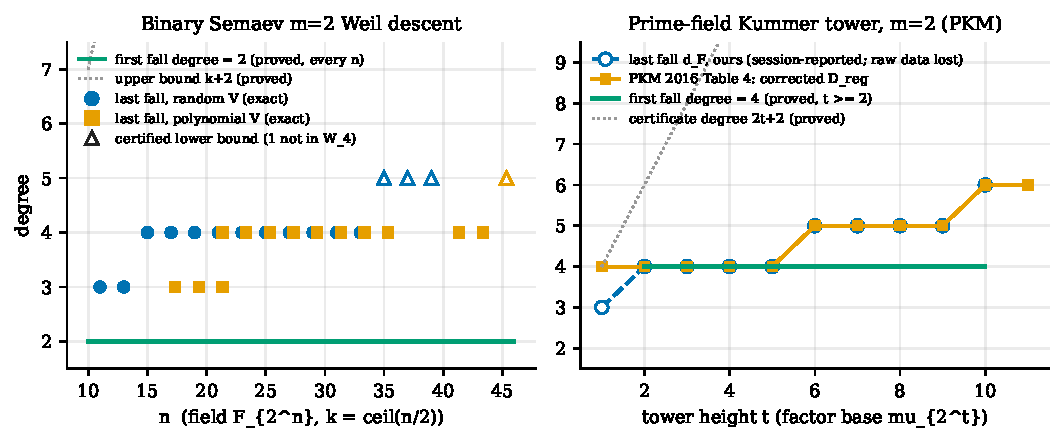
\includegraphics[width=\linewidth]{figures/fig-fall-degrees.pdf}
\caption[]{\emph{Left:} binary Semaev $m=2$ descent. The first fall degree
is 2 (Corollary~\ref{cor:ffd2}, proved). Filled marks are exact last fall
degrees per unsatisfiable instance. Open triangles are certified lower
bounds $d_{\tilde F}\ge5$ (Theorem~\ref{thm:lfd5}). The dotted line is the
proved upper bound $k+2$. \emph{Right:} prime-field Kummer tower, $m=2$
(\S\ref{sec:fd-pkm}). The session-reported last fall degree lies on the
corrected degree of regularity of PKM 2016, Table~4. The first fall degree
is 4 (proved). Values and sources: \art{figures/data-new.json}.}
\label{fig:fd}
\end{figure}

\begin{theorem}[Exact last fall degrees; computer-verified on instances]\label{thm:lfdexact}
On the diagonal $k=\lceil n/2\rceil$:
\begin{itemize}
\item $d_{\tilde F}=3$ on all six random-subspace instances at $n=11,13$
  and on all ten polynomial-subspace instances at $n=17,19$;
\item $d_{\tilde F}=4$ on all 29 random-subspace instances with
  $15\le n\le33$, and on all 25 polynomial-subspace instances with
  $23\le n\le35$ or $n=41,43$;
\item $d_{\tilde F}=4$ on Semaev's own cell ($n=40$, $k=20$, uniform $z$),
  matching his reported $d_{F4}=4$;
\item $d_{\tilde F}=5$ exactly on instance R35a ($n=35$, $k=18$, random
  $V$): $1\notin W_4$, and both restrictions $a_1=0,1$ are refuted at
  $W_4$ (Lemma~\ref{lem:branch}).
\end{itemize}
\end{theorem}

Table~\ref{tab:fd-binary} gives every instance behind
Theorems~\ref{thm:lfdexact} and~\ref{thm:lfd5}, one row per subspace family
and $n$, in the layout of Kousidis and Wiemers' Table~1.

\begin{table}[p]
\centering\small
\begin{tabular}{@{}clrrrrrrrr@{}}
\toprule
$m$ & $V$ & $n$ & $k$ & inst. & $D_{\rm ff}$ & $d_{\tilde F}$ & cols at $D=4$ & s at $D=4$ & codim $W_4\ge$ \\
\midrule
2 & P & 17 & 9 & 6 & 2 & 3 &  &  &  \\
 &  & 19 & 10 & 4 & 2 & 3 &  &  &  \\
 &  & 21 & 11 & 4 & 2 & 3$\times$2, 4$\times$2 & 9{,}109 & 7.3 &  \\
 &  & 23 & 12 & 4 & 2 & 4 & 12{,}951 & 7.3 &  \\
 &  & 25 & 13 & 4 & 2 & 4 & 17{,}902 & 11.1 &  \\
 &  & 27 & 14 & 4 & 2 & 4 & 24{,}158 & 20.3 &  \\
 &  & 29 & 15 & 3 & 2 & 4 & 31{,}931 & 40.9 &  \\
 &  & 31 & 16 & 3 & 2 & 4 & 41{,}449 & 51.9 &  \\
 &  & 33 & 17 & 3 & 2 & 4 & 52{,}956 & 100.1 &  \\
 &  & 35 & 18 & 2 & 2 & 4 & 66{,}712 & 160.9 &  \\
 &  & 41 & 21 & 1 & 2 & 4 & 124{,}314 & 1076.1 &  \\
 &  & 43 & 22 & 1 & 2 & 4 & 149{,}986 & 2001.3 &  \\
 &  & 45 & 23 & 1 & 2 & $\ge5$ & 179{,}447 & 1850.7 & 12{,}742 \\
\addlinespace
 & S & 40 & 20 & 2 & 2 & 4 & 102{,}091 & 537.9 &  \\
\addlinespace
 & R & 11 & 6 & 3 & 2 & 3 &  &  &  \\
 &  & 13 & 7 & 3 & 2 & 3 &  &  &  \\
 &  & 15 & 8 & 3 & 2 & 4 & 2{,}517 & 1.0 &  \\
 &  & 17 & 9 & 3 & 2 & 4 & 4{,}048 & 1.3 &  \\
 &  & 19 & 10 & 3 & 2 & 4 & 6{,}196 & 2.1 &  \\
 &  & 21 & 11 & 3 & 2 & 4 & 9{,}109 & 3.2 &  \\
 &  & 23 & 12 & 3 & 2 & 4 & 12{,}951 & 4.1 &  \\
 &  & 25 & 13 & 3 & 2 & 4 & 17{,}902 & 6.6 &  \\
 &  & 27 & 14 & 3 & 2 & 4 & 24{,}158 & 15.4 &  \\
 &  & 29 & 15 & 3 & 2 & 4 & 31{,}931 & 24.0 &  \\
 &  & 31 & 16 & 3 & 2 & 4 & 41{,}449 & 45.2 &  \\
 &  & 33 & 17 & 2 & 2 & 4 & 52{,}956 & 91.9 &  \\
 &  & 35 & 18 & 2 & 2 & $\ge5$ & 66{,}712 & 121.0 & 5{,}287 \\
 &  & 37 & 19 & 2 & 2 & $\ge5$ & 82{,}993 & 312.9 & 10{,}066 \\
 &  & 39 & 20 & 2 & 2 & $\ge5$ & 102{,}091 & 445.9 &  \\
\addlinespace
 & U & 33 & 17 & 2 & 2 & 4 & 52{,}956 & 95.4 &  \\
 &  & 35 & 18 & 2 & 2 & $\ge5$ & 66{,}712 & 126.4 & 5{,}287 \\
\addlinespace
 & T & 29 & 15 & 2 & 2 & 4 & 31{,}931 & 38.3 &  \\
 &  & 31 & 16 & 2 & 2 & 4 & 41{,}449 & 68.3 &  \\
 &  & 33 & 17 & 2 & 2 & $\ge5$ & 52{,}956 & 128.8 & 4{,}888 \\
\bottomrule
\end{tabular}

\caption[]{Binary Weil descent of $\Sem3$ ($m=2$, $k=\lceil n/2\rceil$): the
first fall degree $D_{\rm ff}=2$ (Corollary~\ref{cor:ffd2}, proved for
every $n$) beside the last fall degree $d_{\tilde F}$, the least $D$ with
$1\in W_D$, for each instance. Subspace families: P, Semaev's polynomial
subspace $\langle1,t,\ldots,t^{k-1}\rangle$; S, the same with uniform $z$
(Semaev's own cell); R, random; U, random with uniform $z$; T, random inside
$\ker\operatorname{Tr}$. ``$\ge5$'' means $1\notin W_4$; R35a is exactly 5
(Theorem~\ref{thm:lfdexact}). Columns: instances; columns of the degree-4 closure
matrix; median closure wall time at
$D=4$ in seconds, over the instances run to that degree (host not
recorded); certified codimension of $W_4$ where an independent certificate
was checked. Source:
\art{crypto-autoresearcher:analysis/semaev-m2-last-fall-degree/results/},
laid out by \art{figures/make_tab_fall_degrees.py} from
\art{figures/data-falldegree-instances.json}.}
\label{tab:fd-binary}
\end{table}

\begin{theorem}[Certified $d_{\tilde F}\ge5$]\label{thm:lfd5}
For each instance below, a certificate (Proposition~\ref{prop:cert}) for
$1\notin W_4(F)$ was accepted by the independent checker. Hence
$d_{\tilde F}\ge5$, and every F4 run reaches degree $\ge5$.

\smallskip\noindent
\begin{tabular}{@{}lllll@{}}
\toprule
instance & $n$ & $k$ & subspace & certified $\operatorname{codim}W_4\ge$ \\
\midrule
T33a, T33b & 33 & 17 & random $\subset K_0$ & 4{,}888 \\
R35a, R35b, U35a, U35b & 35 & 18 & random (U: uniform $z$) & 5{,}287 \\
Q35a, Q35b (satisfiable) & 35 & 18 & random & 5{,}287 \\
R37a, R37b & 37 & 19 & random & 10{,}066 \\
P45a & 45 & 23 & Semaev's default $\langle1,t,\ldots,t^{22}\rangle$ & 12{,}742 \\
C19a, C19b (chain $m=t=3$) & 19 & 7 & random & 9{,}253, 6{,}817 \\
\bottomrule
\end{tabular}

\smallskip\noindent
Two further instances, R39a and R39b ($n=39$), and C21a and C21b (the
chain at $n=21$) have $1\notin W_4$ by implementation~A alone.
\end{theorem}

For Q35a and Q35b, which have 6 and 2 Boolean solutions, the bound follows
from Proposition~\ref{prop:bridges}(4), since $5{,}287\gg|S|$. The P45a
closure stalls after three rounds at
$\dim W_4\cap B_{\le d}=(0,1,224,8950,166705)$, out of 179{,}447
monomials. Its quadratic part, $224=5n-1$, is exactly the
polynomial-subspace count of Lemma~\ref{lem:deg3}: at degree 4 the closure
finds no new falls.

\begin{corollary}[Semaev's Assumption 1 fails as stated]\label{cor:assump}
Semaev's Assumption~1~\cite[\S4.5]{semaev2015} asserts $d_{F4}\le4$ for
Boolean systems equivalent to his system (5), for $q=2^n$,
$k=\lceil n/m\rceil$, any subspace of dimension $k$ and any $2\le t\le m$.
Theorem~\ref{thm:lfd5} contradicts it in three cells:
\begin{itemize}
\item $(n,m,t,k)=(35,2,2,18)$, with random subspaces;
\item $(45,2,2,23)$, with his own default subspace;
\item $(19,3,3,7)$ and $(21,3,3,7)$, inside the parameter range of his
  tables, where his polynomial subspace gives 4 and random subspaces do
  not.
\end{itemize}
\end{corollary}

Table~\ref{tab:fd-chain} lists the chain instances. With Semaev's
polynomial subspace the closure refutes at degree~4 in every cell; with
random subspaces it does not at $n=19,21$.

\begin{table}[t]
\centering\small
\begin{tabular}{@{}lccrrlrrr@{}}
\toprule
instance & $m=t$ & $V$ & $n$ & $k$ & $d_{\tilde F}$ & cols at $D=4$ & s at $D=4$ & codim $W_4\ge$ \\
\midrule
D17a & 3 & P & 17 & 6 & $\le$4 & 59{,}536 & 294.6 &  \\
D17b & 3 & P & 17 & 6 & $\le$4 & 59{,}536 & 297.4 &  \\
D19a & 3 & P & 19 & 7 & $\le$4 & 102{,}091 & 1283.7 &  \\
D19b & 3 & P & 19 & 7 & $\le$4 & 102{,}091 & 1047.1 &  \\
D21a & 3 & P & 21 & 7 & $\le$4 & 124{,}314 & 1270.3 &  \\
D21b & 3 & P & 21 & 7 & $\le$4 & 124{,}314 & 1225.4 &  \\
C17a & 3 & R & 17 & 6 & $\le$4 & 59{,}536 & 281.3 &  \\
C17b & 3 & R & 17 & 6 & $\le$4 & 59{,}536 & 270.9 &  \\
C19a & 3 & R & 19 & 7 & $\ge$5 & 102{,}091 & 1088.5 & 9{,}253 \\
C19b & 3 & R & 19 & 7 & $\ge$5 & 102{,}091 & 1184.4 & 6{,}817 \\
C21a & 3 & R & 21 & 7 & $\ge$5 & 124{,}314 & 1806.2 &  \\
C21b & 3 & R & 21 & 7 & $\ge$5 & 124{,}314 & 1790.4 &  \\
\bottomrule
\end{tabular}

\caption[]{Chained system, $m=t=3$, $k=\lceil n/3\rceil$: closure at $D=4$
per instance. ``$\le4$'' means $1\in W_4$; ``$\ge5$'' means $1\notin W_4$.
Certified codimensions as in Table~\ref{tab:fd-binary}; C21a and C21b have
no checked certificate: $1\notin W_4$ by implementation~A alone. Source:
\art{crypto-autoresearcher:analysis/semaev-m2-last-fall-degree/results/instances_t3.json}.}
\label{tab:fd-chain}
\end{table}

\paragraph{What is new, and what is not.} That the degree of regularity
reaches 5 has been \emph{observed} before:
\begin{itemize}
\item Kosters and Yeo saw Magma step degrees of $\ge5$ at $n=40$ and
  $n=45$~\cite{kosters2015notes};
\item Kousidis and Wiemers saw F4 at step degree 5 for $n=37$--$48$, $m=2$,
  and wrote that a lower bound on the degree of regularity ``can
  potentially answer an open question''~\cite{kousidis2019}.
\end{itemize}
Table~\ref{tab:fd-kw} sets their $m=2$ rows beside ours at the same
$n$. The quantities differ: $D_{\rm reg}$ is the highest step degree of
their F4 runs, while $d_{\tilde F}$ is the closure degree of the system,
and no F4 run refutes below it. So their $5$ at $n=41,43$ against our $4$
on polynomial subspaces is not a contradiction; F4 overshoots the closure
there. At $n=35$ their $D_{\rm reg}=4$ agrees with our polynomial subspace
and differs from every random subspace we drew, which are all $\ge5$:
which subspace a table uses decides the degree it reports. At $n=45$ both
reach 5.

\begin{table}[t]
\centering\small
\begin{tabular}{@{}rrrrrrcc@{}}
\toprule
\multicolumn{6}{c}{Kousidis--Wiemers, Table 1 ($m=2$, F4)} & \multicolumn{2}{c}{this work, $d_{\tilde F}$} \\
\cmidrule(r){1-6}\cmidrule(l){7-8}
$n$ & $n'$ & $D_{\rm ff}$ & $D_{\rm reg}$ & s & GB & P or S & R, U or T \\
\midrule
34 & 17 & 2 & 4 & 188 & 1.2 &  &  \\
35 & 18 & 2 & 4 & 1{,}237 & 16.1 & 4 & $\ge5$$^{\rm R}$; $\ge5$$^{\rm U}$ \\
36 & 18 & 2 & 4 & 1{,}342 & 16.4 &  &  \\
37 & 19 & 2 & 5 & 2{,}542 & 29.2 &  & $\ge5$$^{\rm R}$ \\
38 & 19 & 2 & 5 & 2{,}815 & 25.2 &  &  \\
39 & 20 & 2 & 5 & 4{,}785 & 45.6 &  & $\ge5$$^{\rm R}$ \\
40 & 20 & 2 & 5 & 4{,}858 & 46.3 & 4$^{\rm S}$ &  \\
41 & 21 & 2 & 5 & 7{,}930 & 65.3 & 4 &  \\
42 & 21 & 2 & 5 & 8{,}901 & 66.7 &  &  \\
43 & 22 & 2 & 5 & 16{,}816 & 95.5 & 4 &  \\
44 & 22 & 2 & 5 & 15{,}690 & 96.8 &  &  \\
45 & 23 & 2 & 5 & 38{,}352 & 140.0 & $\ge5$ &  \\
46 & 23 & 2 & 5 & 31{,}735 & 140.7 &  &  \\
47 & 24 & 2 & 5 & 103{,}200 & 207.7 &  &  \\
48 & 24 & 2 & 5 & 86{,}636 & 208.2 &  &  \\
\bottomrule
\end{tabular}

\caption[]{The $m=2$ rows of Kousidis and Wiemers' Table~1~\cite{kousidis2019}
(F4, averages over ten repetitions; $n'=\lceil n/2\rceil$; time in
seconds, memory in GB), transcribed from the published table, beside the
last fall degree of our instances at the same $n$
(Table~\ref{tab:fd-binary}). Superscripts give the subspace family. Their
$m=3,4$ rows ($D_{\rm ff}=D_{\rm reg}=7$ and $13$, $n\le21$) concern
$\Sem4$ and $\Sem5$ and have no counterpart here.}
\label{tab:fd-kw}
\end{table}

Those are properties of solver runs. Theorem~\ref{thm:lfd5} is a property
of the systems, carried by a certificate any reader can check. With
Corollary~\ref{cor:ffd2} it makes the separation between first and last
fall degree rigorous on named instances. What remains open is the same
as before: a proof that $d_{\tilde F}\to\infty$. Semaev's asymptotics
survive if the regularity degree is $o(\sqrt{n\ln n})$, so only a growing
lower bound bears on the subexponential claim.

\paragraph{Re-verification.} For this treatise, the T33a certificate was
regenerated from the committed producer (M4RI 20200125, 4\,min 40\,s on
4~vCPUs) and checked with \texttt{cert\_check.py}:
\begin{itemize}
\item the certificate is byte-identical to the recorded SHA-256
  \texttt{cf9dcae8\ldots22cf};
\item the checker reports ``1 is not in $W_4(F)$, and
  $\operatorname{codim}W_4(F)\ge4888$'' (38.8\,s);
\item the closure dimensions $(0,0,64,2968,48068)$ match the record.
\end{itemize}
Source: \art{research/paper_opportunities_20261029/REPORT.md}, \S6.

\section{Explicit membership over any field: the guarded chain}\label{sec:fd-guarded}

A second presentation encodes factor-base membership directly. Let $S$ be
a set of $B$ abscissae of rational points, and $g(T)=\prod_{s\in S}(T-s)$.
The two-$\Sem3$ chain with an inverse guard is
\[
  F_S=\{g(x),\ g(y),\ g(z),\ \Sem3(x,y,u),\ \Sem3(u,z,r),\ v(x-y)-1\},
\]
with $r=x(R)$. Degrees are ordinary total degrees with explicit inputs.
The first fall degree is the homogeneous-top syzygy degree modulo Koszul
syzygies. Source: \art{research/guarded_fall_degree_20261028/}, which holds
written proofs, independent audits, a native exact replay and partial
Lean.

\begin{theorem}[Guarded chain]\label{thm:guarded}
For unsatisfiable instances:
\begin{enumerate}
\item Short Weierstrass curves, $p>3$, $B=3$:
  $(d_{\rm ff},d_F)=(4,5)$, \emph{exactly}, for every $p$.
\item Same presentation, any $B\ge3$: $d_{\rm ff}=B+1$ and
  $\max(5,B+1)\le d_F\le3B-4$.
\item Ordinary binary curves $Y^2+XY=X^3+a_2X^2+a_6$, $B=3$:
  \begin{itemize}
  \item $d_F=4$ if and only if $g=T^3+c$, which is possible only for even
    $n$;
  \item $d_F=5$ otherwise.
  \end{itemize}
  So for odd $n$, which covers every SEC~2 binary size, every
  unsatisfiable instance has $(4,5)$.
\item Binary curves, $B\ge4$: $B+1\le d_F\le3B-4$.
\end{enumerate}
\end{theorem}

\begin{proof}[Proof sketch of (1)]
\emph{Upper bound.} The divided difference
$Q=(g(x)-g(y))/(x-y)$ enters $V_4$ through the guard. The pair is then
replaced by the missing root $w=s_1-x-y$. The two quadratics in $u$ are
normalised and their resultant extracted in stages inside $V_5$. Finally
the unit $T(w,z)$ is inverted in $K[w,z]/(g(w),g(z))\cong K^9$.

\emph{Lower bound.} The space $W=(I_0\cap R_{\le4})+Kf_1+Kf_2$ is closed
under the degree-4 operations and excludes 1. This uses characteristic
$>3$, through $-3\ne0$.
\end{proof}

Exact degree-5 refutation DAGs were replayed in native arithmetic on public
fixtures:
\begin{itemize}
\item $p=101$ and $p=5$;
\item secp256k1, P-256, P-384 and P-521, with $S=\{x(G),x(2G),x(4G)\}$ and
  $R=16G$; the DAGs have 413--415 nodes, and OpenSSL rechecks the points.
\end{itemize}
Twenty polynomial identities used in the proofs are checked in Lean
(\texttt{FallDegreeIdentities.lean}, \texttt{PrimeBitLocal.lean}; axioms
\texttt{propext} and \texttt{Quot.sound} only). The degree-4 lower bound
is now machine-checked: \texttt{GuardedModel.no\_degree\_four\_refutation}
proves that 1 is not derivable at degree four from the six generators, over
every field with $6\ne0$ and three distinct base abscissae, and
\texttt{lastFall\_lower} states the last-fall consequence under an explicit
unit-ideal hypothesis (\art{research/guarded_fall_degree_20261028/formal/GuardedModel.lean};
six modules, fresh \texttt{leanchecker} replays and a transitive axiom audit,
merged in \#2814). The degree-5 upper construction, the bridge from rational
unsatisfiability to the unit ideal, and the first-fall syzygy statement are
\emph{not} formalised, so the exact pair $(4,5)$ is not yet a Lean theorem. A
\texttt{lastFallDegree} definition and Caminata--Gorla's Theorem~2.8 in
\art{crypto-autoresearcher:formal/CryptoResearch/FallDegree/LastFall.lean}
are the bridge a complete formalisation would build on.

Two Boolean upper bounds accompany the guarded chain:
\begin{itemize}
\item $d_F\le3\ell+1$ for the fully Boolean binary encoding, with $\ell$
  bits per base coordinate;
\item $d_F\le3\ell+2$ for a prime-field bit-restricted lookup encoding.
\end{itemize}
Both are instances of the standard brute-force refutation in Polynomial
Calculus~\cite{cei1996}: fix the base bits, and refute the affine residue.
For the binary chain at $t=3$ they are weaker than Theorem~\ref{thm:upper}'s
$2k+3$.

\section{Prime-field Kummer towers}\label{sec:fd-pkm}

Petit, Kosters and Messeng~\cite{pkm2016} take the factor base
$V=\mu_{2^t}$ over $\FF_p$ (with $2^t\mid p-1$). They write membership as a
tower $y_0=x/g$, $y_{j+1}=y_j^2$, $y_{t-1}^2=1$, and argue the complexity
from the first fall degree. Source for this section:
\art{research/prime_fall_degree_20261027/DERIVED.md}, written proofs D1--D8.

\begin{theorem}[Kummer towers, $m=2$]\label{thm:pkm}
Let $R=\FF_p[y]/T$ be the tower quotient. Items (3)--(5) concern
\emph{inconsistent} systems, those whose reduced $\Sem3$ is a unit of $R$; a
satisfiable target has no inverse in $R$, and the refutation bounds do not
apply to it.
\begin{enumerate}
\item $T$ is a Gröbner basis, and $R\cong\FF_p^{V^m}$. So every ideal
  over $R$ is radical, and an $m=2$ system is inconsistent if and only if
  the reduced $\Sem3$ is a unit of $R$.
\item $R=\FF_p[z]/(z^K-1)$ with $K=2^t$. The degree of a monomial $z^k$ is
  $\operatorname{popcount}(k)$, and degree falls are exactly binary
  carries.
\item If $t\ge2$, $g\ne0$, $3x_R^2+a\ne0$ and the system is inconsistent, then $d_{\rm ff}=4$
  (operational convention), for every $t$. The degree-2 part of $f$ is a
  bilinear form with $\det M=-2g^6(3x_R^2+a)\ne0$, so nothing falls at 3;
  the monomial $q=y_{10}y_{11}$ gives a fall at 4.
\item For an inconsistent system, the no-fall certificate has degree
  $d_F\le2+\operatorname{popdeg}(f^{-1})\le2t+2$.
\item For an inconsistent system in the naive presentation
  $\{\Sem3,\ x_i^K-g^K\}$ of the \emph{same} set, $d_F\ge2^t$. So $d_F$ is not an invariant of the ideal; it depends
  on the presentation.
\item A single summand has $d_F=2$ for every $t$. Growth at $m=2$ must
  therefore come from the genus-one curve $f(z_1,z_2)=0$; no
  specialisation to finitely many points can show it.
\end{enumerate}
\end{theorem}

\paragraph{Measured, and prior.} Table~\ref{tab:fd-pkm} sets the study's
session-reported median last fall degree for $t=1..10$ at
$p=2{,}013{,}265{,}921$ beside the corrected degree of regularity in PKM's
own Table~4 for $n_1=1..11$ (also Figure~\ref{fig:fd}, right). The raw
records were never committed (the study's \texttt{RESTART.md}), so the
$d_F$ column is session-reported, not re-derivable. From $t=2$ on the two
columns coincide.

\begin{table}[t]
\centering\small
\begin{tabular}{@{}rrrr@{}}
\toprule
$t$ (PKM: $n_1$) & $D_{\rm ff}$ (proved) & $d_F$ (session median) & PKM $D_{\rm reg}^{\rm corr}$ \\
\midrule
1 &  & 3 & 4 \\
2 & 4 & 4 & 4 \\
3 & 4 & 4 & 4 \\
4 & 4 & 4 & 4 \\
5 & 4 & 4 & 4 \\
6 & 4 & 5 & 5 \\
7 & 4 & 5 & 5 \\
8 & 4 & 5 & 5 \\
9 & 4 & 5 & 5 \\
10 & 4 & 6 & 6 \\
11 &  &  & 6 \\
\bottomrule
\end{tabular}

\caption[]{Prime-field Kummer tower, $m=2$, factor base $\mu_{2^t}$:
the proved first fall degree (Theorem~\ref{thm:pkm}(3); it needs $t\ge2$),
the session-reported median last fall degree at $p=2{,}013{,}265{,}921$
(raw data not committed), and the corrected degree of regularity
$D_{\rm reg}^{\rm corr}$ of Petit, Kosters and Messeng, Table~4
(prime case)~\cite{pkm2016}. Source: \art{figures/data-new.json}, from
\art{research/prime_fall_degree_20261027/}.}
\label{tab:fd-pkm}
\end{table} So the \emph{growth} is prior art. What
Theorem~\ref{thm:pkm} adds is the proved constant first fall degree beside
it, and the presentation dependence. A prediction,
$d_F=4+\lfloor(t-2)/4\rfloor$, was registered before any $t\ge11$ row and
is untested.

\section{Measured solving degrees in other presentations}

The binary programme measured refutation and closure degrees on many
presentations; the full record is in~\cite[\S6]{icprogram2026}.
Table~\ref{tab:fd-other} lists the last fall degree by base-subspace
dimension $\ell$. It is flat in $n$ at fixed $(m,\ell)$ and rises with
$\ell$.

\begin{table}[t]
\centering\small
\begin{tabular}{@{}rrcc@{}}
\toprule
$m$ & $\ell$ & $n$ & $d_F$ \\
\midrule
3 & 5 & 10--15 & 4 \\
  & 6 & 16--24 & 4 \\
  & 7 &        & $\ge5$ (every draw) \\
\addlinespace
4 & 3 & 9--14  & 4 \\
\addlinespace
5 & 3 & 11--15 & 4 \\
\bottomrule
\end{tabular}
\caption[]{Binary decomposition systems in other presentations: last fall
degree $d_F$ by $m$ and base-subspace dimension $\ell$, over the measured
range of $n$. At $(m,\ell)=(3,7)$ every draw is refuted only at degree
$\ge5$. Source:~\cite[\S6]{icprogram2026}.}
\label{tab:fd-other}
\end{table}

Three further measurements bear on the solver rather than the system:
\begin{itemize}
\item \emph{Plain refutation tracks the semi-regular degree.} The plain
  Macaulay refutation degree stays within one of the semi-regular
  prediction in all 14 exact cells.
\item \emph{Closure algorithms refute one or two degrees earlier.} A
  MutantXL-style closure refutes all 92 unsatisfiable draws at degree 3--4,
  where XL needs 5--7.
\item \emph{Guessing variables restores degree 4.} Fixing one or two
  variables restores degree 4 at $(m,\ell)=(3,7)$, at $1/116$--$1/260$ of
  the projected degree-5 cost.
\end{itemize}
Every observed growth is growth in the size of the factor base: in $\ell$,
$k$, $t$, $B$, or the digit count $s$ of a prime digit presentation (where
$d_{\rm ff}=d_F=4+\lfloor s/2\rfloor$ at $m=2$, reproduced by a curve-free
null). None was observed in $n$ at a fixed base.

\section{What this settles and what it does not}\label{sec:fd-summary}

\begin{itemize}
\item \emph{Settled.} In the three presentations the programme studied,
  the first fall degree is a proved constant of the presentation: 2 for
  binary Weil descent, $B+1$ for explicit membership, 4 for Kummer
  towers. The last fall degree is not bounded by it.
  \begin{itemize}
  \item This is proved for the guarded chain at $B=3$ (exactly 5 against
    4).
  \item It is certified on named binary instances: $\ge5$ against 2, at
    $n=33$--$45$ and in the $m=t=3$ chain.
  \item It is measured for Kummer towers (6 against 4 at $t=10$).
  \end{itemize}
  Any complexity argument that substitutes the first fall degree for the
  solving degree is unsupported for these systems.
\item \emph{Not settled.} No presentation has a proved last-fall lower
  bound that grows with $n$. That is the open problem of
  HKY~\cite{hky2015} and Kousidis--Wiemers~\cite{kousidis2019}, and the
  only result that would bear on the subexponential claims. The upper
  bounds $k+2$ and $(t-1)k+t$ are linear in $n$, far above every observed
  value.
\item \emph{Missing before submission.} The certificates are committed
  only as hashes; they regenerate (above) but need public hosting. The
  sample is small: two instances per $n$ at $n\ge33$, one polynomial
  instance at $n\ge41$. The written proofs need expert review. The
  Kummer-tower data must be regenerated
  (\art{research/paper_opportunities_20261029/}).
\end{itemize}

\chapter{Obstructions: what moving the problem cannot buy}\label{ch:obstructions}

The programme kept 148 leads against ECDLP in a lead atlas
(\art{crypto-autoresearcher:knowledge/leads/ecdlp/}, reviewed 2026-10-24).
Of these:
\begin{itemize}
\item 73 are closed with a named obstruction;
\item 51 are open with a decided next step;
\item 16 are blocked;
\item 8 are unexamined.
\end{itemize}
Most obstructions are textbook results applied to the case at hand: the
Shoup--Nechaev generic bound, the Corrigan-Gibbs--Kogan preprocessing bound
$ST^2\gtrsim N$~\cite{cgk2018}, isogeny invariance of the group order, and
the Balasubramanian--Koblitz embedding-degree bound. This chapter records
the few that the programme \emph{proved} itself and that constrain index
calculus specifically. Each states a lever that cannot work, and why.

\section{Transport conservation}\label{sec:obs-transport}

A homomorphic transfer $\varphi:E\to E'$ with rational kernel $\kappa$
changes the number of ordered $m$-decompositions of a target by exactly
$\abs{\kappa}^{m-1}$ (Lemma~\ref{lem:conservation} in
Chapter~\ref{sec:transfer}). So an isogeny buys only three things:
\begin{itemize}
\item the kernel symmetry, which is trivial on prime-order curves;
\item the factor-base geometry available on the destination curve;
\item the cost of arithmetic there.
\end{itemize}
Chains of isogenies compose to one homomorphism. A loop is an endomorphism
acting as a known scalar. Multi-curve factor bases glued by isogenies are
single-curve bases in disguise. Measured across sizes at fixed cofactor,
fibre-aware index calculus loses ground to rho as $\#E^{1/6}$; the full
measurements are in Chapter~\ref{sec:transfer}.

\section{The summation cover is the same everywhere}

Chapter~\ref{ch:cover} proved:
\begin{itemize}
\item the monodromy of the summation cover is $(\ZZ/2)^{m-2}$ for every
  curve;
\item its fibres split completely on the factor-base locus;
\item mean yield at fixed base size is a double count.
\end{itemize}
Together these close three families of leads: curve selection by
anomalous monodromy, fibre censuses as a relation-rate probe, and
factor-base geometries claimed to raise yield.

\section{Oracle-augmented index calculus stays generic}

Several leads proposed giving index calculus an extra oracle on the group:
\begin{itemize}
\item a jet or $p$-adic lift;
\item an endomorphism;
\item an incidence or halving test;
\item an elliptic-net evaluation.
\end{itemize}
The programme proved, at derivation tier, that each of these is
simulable in the generic group model, so it cannot beat
$\sqrt r$ (\texttt{KN-FIND-002}, \texttt{KN-FIND-b7e091},
\texttt{KN-FIND-194294}; halving is equivalent to an $x$-coordinate oracle).

The minimal non-simulable order-based identifier is a threshold oracle
$C_t$ (\texttt{KN-FIND-982fdf}). Table-based decomposition then obeys the
preprocessing bound $ST^2\gtrsim N$. Balanced generic index calculus costs
about $r^{2/3}/n^{4/3}$, consistent with the measured growth of the Koblitz
gap to rho as $r^{0.165\,[0.117,0.213]}$
(\texttt{LEAD-ICB-generic-table-oracle}). These are known instances of
generic-group reasoning~\cite{cgk2018}; they are recorded because each
retired a concrete proposal.

\section{Lifting sections does not produce relations}

Silverman's xedni calculus lifts points to a curve over a global field, in
the hope that rank forces relations. On a frozen family of rational
elliptic surfaces (with $\deg b=6$ and monic quadratic $x$), the programme
derived the exact lift probability
\[
  P_{\rm lift}(p)=\frac{1-2/p+p^{-3}}{2p^3},
\]
so the exponent is $\alpha=3$, far above the $\alpha<1/2$ that a relation
source would need. This was checked against $596{,}268{,}874$ enumerated
slots with no disagreement, and a parameter count reproduces $\alpha=3$
(\texttt{LEAD-ICP-xedni-function-field-sections}, \texttt{EV-XEDN-001}).
The scope is one family ($\deg b\le10$, $p\le31$). A dimension-count theorem
over all section shapes would be needed to close the route in general.

\section{Twist points carry no relations}

A curve and its quadratic twist share $x$-coordinates, and therefore share
summation polynomials. Could twist points supply relations for the curve?
They cannot. Frobenius acts as $+1$ on $E(\FF_q)$ and as $-1$ on the
embedded twist, so the twist part $B$ of any sum satisfies $2B=0$.

The study \art{research/twist_obstruction_20261026/} checked this
exactly on toy binary curves in the ECC2K-130 model (odd $n$, twist
$a\mapsto a+1$):
\begin{itemize}
\item 0 of 356{,}530{,}036 mixed sums are rational;
\item 0 violations on 4{,}954 decomposition targets at $m=2,3$;
\item the off-parity solution sets equal the predicted ones on 1{,}154 of
  1{,}154 targets;
\item positive controls found all 18{,}042 and 95 planted solutions.
\end{itemize}
A heuristic that ignored the obstruction predicted that 74--89\% of
solutions would contain a twist-lifting coordinate; 0\% did at $m=2$.

A follow-up asked whether a factor-base subspace can \emph{avoid} the twist
altogether (\art{research/lift_dense_factor_base_20261027/}; 11 Lean
theorems, standard axioms only).
\begin{itemize}
\item \emph{Composite degree $N=dn$, $n\ge3$: yes.} On suitable
  $\FF_{2^d}$-lines the lift condition collapses to the constant
  $\operatorname{Tr}(a)$. When $\operatorname{Tr}(a)=0$ every abscissa
  lifts, giving $2^n$ relations per Gaudry--Diem trial. This applies to
  c2pnb208w1 and c2pnb368w1, but the modelled gain is $+0.50$ bits, a
  model output, not a measurement.
\item \emph{Prime degree (ECC2K-130): this construction does not exist.}
  A prime-degree field has no proper intermediate subfield, so there are no
  $\FF_{2^d}$-lines to use. This does not rule out other twist-avoiding
  subspaces. At the small prime degrees tested, all-lift subspaces of
  dimension 4--5 exist, though fewer than for density-paired random sets
  (exact all-lift 4-subspace counts $0.921\pm0.018$ of the null at $N=11$,
  permutation $p=2\cdot10^{-5}$). This is toy evidence. Whether useful
  twist-avoiding subspaces exist at cryptographic prime degree is
  unresolved.
\end{itemize}

\section{What the obstructions leave open}

None of the obstructions above concerns the cost of \emph{solving} the
decomposition system, nor the linear algebra. Chapter~\ref{ch:falldegree}
shows that the solving cost is genuinely open. The algorithms of
Part~\ref{part:algorithms} attack the remaining free terms.


\part{Algorithms and measurements}\label{part:algorithms}
\chapter{Root-finding decomposition}\label{sec:rootfinding}

\section{Origin: a suggestion in an audited manuscript}

The textbook decomposition oracle builds Semaev's polynomial system and
solves it with a Gr\"obner-basis engine. On 12 October a 13-page manuscript,
\emph{Point Decomposition by Root Finding}, was supplied for assessment. We
froze it (\art{research/ecbench_rootfinding_assessment_20261012/source-paper.pdf},
SHA-256 \texttt{743d3d3e\ldots7c01}) and audited it against its source
branch before measuring anything. Its central suggestion is simple: for two
summands, fixing one factor-base point turns $\Sem3$ into a quadratic in the
remaining variable whose roots are already known.

\begin{proposition}[roots of $\Sem3$]\label{prop:s3}
Let $E: y^2=x^3+ax+b$ over a field $K$ of characteristic $\ne2,3$, and let
$R,F\in E(K)$ be affine with $x_R\ne x_F$. Then
\[
  \Sem3(x_R,x_F,X)=(x_R-x_F)^2\,(X-x_+)(X-x_-),\qquad
  x_\pm=x(R\pm F),
\]
so $\Sem3(x_R,x_F,X)=0$ iff $X\in\{x(R+F),x(R-F)\}$.
\end{proposition}
\begin{proof}[Proof sketch]
With $\lambda_\pm=(\pm y_F-y_R)/(x_F-x_R)$ the chord slopes,
$x_\pm=\lambda_\pm^2-x_R-x_F$. Expanding $(X-x_+)(X-x_-)$ and eliminating
$y_R^2,y_F^2$ with the curve equation gives exactly Semaev's
$\Sem3/(x_R-x_F)^2$. The identity is machine-checked over an arbitrary
field in Lean 4 with Mathlib (\art{papers/rootfinding-decomposition/lean/S3Roots.lean},
theorems \texttt{SemaevS3.S3\_factor} and \texttt{SemaevS3.S3\_root\_iff};
no \texttt{sorry}; axioms \texttt{propext}, \texttt{Classical.choice},
\texttt{Quot.sound}).
\end{proof}

Hence the two-summand system has a parametrised variety: $R=\pm F_i\pm F_j$
iff $x(R\mp F_i)\in x(\Fb)$. No polynomial system is solved; the oracle is
one subtraction and one table probe per base point.

\paragraph{Prior art.} Neither the identity nor the oracle is new. The
identity is a direct consequence of how $\Sem3$ is defined: it is the
polynomial whose roots are the abscissae of $P_1\pm P_2$. The oracle
mechanism---sum $m-1$ factor-base points in the group and test whether the
result lies in the base---is the second algorithm of McGuire and
Mueller~\cite{mcguire2017}, who also evaluate $\Sem m$ by iterated
resultants instead of solving it, building on the instance-derived bases of
Amadori, Pintore and Sala~\cite{aps2018}. What this section adds is
engineering and measurement: a machine-checked proof, a fail-closed
verification protocol, binary pair-sum tables for up to four summands,
GPU, Kummer-tower and dense-index variants, and complete-cost measurements
in one harness against rho.

\paragraph{What the audit kept and corrected.} The identity is exact under
the stated generic affine condition, and a returned witness can be re-added
in the group for soundness. Completeness of the exhaustive enumeration
holds only with an explicit sign and factor-base convention (the binary
table stores full point keys over a base containing both signs; the
manuscript's schematic $x$-only table needed that convention stated). The
manuscript's NIST baseline was Buchberger, not F4
(\S\ref{sec:corrections}), and its statement that no implementation can
use fewer than linear field operations per ideal fails for repeated
queries against a reusable pair table. Larger-summand enumeration has a
growing exponent in $\abs\Fb$, and the manuscript did not benchmark it end
to end. All of this is recorded in
\art{research/ecbench_rootfinding_assessment_20261012/REPORT.md}.

\section{The algorithms}

\begin{algorithm}[t]
\caption[]{Prime two-summand oracle by direct subtraction}\label{alg:prime}
\begin{algorithmic}[1]
\Require target $R$, base $\Fb=\{F_1,\ldots,F_N\}$, hash set $H$ of
abscissae (or full points) of $\Fb$
\State $d_i\gets x_R-x_{F_i}$ for all $i$; invert all $d_i$ with one
  field inversion and $3(N-1)$ multiplications (Montgomery's trick)
\For{$i=1..N$}
  \For{$\varepsilon\in\{+1,-1\}$}
    \State $\lambda\gets(y_R+\varepsilon y_{F_i})\,d_i^{-1}$;\quad
           $x_3\gets\lambda^2-x_R-x_{F_i}$ \Comment{$x(R-\varepsilon F_i)$}
    \If{$x_3\in H$} recover the sign of $F_j$ from $y_3$; emit
      $R=\varepsilon F_i+\tau F_j$ \EndIf
  \EndFor
\EndFor
\end{algorithmic}
\end{algorithm}

\emph{Prime fields} (Algorithm~\ref{alg:prime},
\art{src/cryptanalysis/prime_fast.rs}): $\Theta(N)$ field operations and
$2N$ lookups per target. \emph{Binary fields}
(\art{src/cryptanalysis/koblitz_index_calculus.rs},
\texttt{DecompositionStrategy::PairTable}, made the default): a precomputed
table of pair sums $F_i+F_j$ turns an $m$-decomposition into $1$, $N$ or
$N^2$ lookups for $m=2,3,4$---the meet-in-the-middle half of a birthday
search, exact and complete like exhaustive search, at the price of
$\Theta(N^2)$ set-up and memory. Both are verified fail closed: every
decomposition is re-added in the group, $\Sem3$ is checked to vanish,
Gr\"obner-variety membership and agreement on refutation are checked
against F4, and planted positive controls must be found.

\section{Generalising the observation}

Over three days the identity was carried through every layer of the
pipeline. Table~\ref{tab:rf-steps} lists the steps; each is its own study
with a protocol registered before it ran.

\begin{table}[t]
\centering\small
\caption[]{Root-finding generalisations, 12--14 October. Every row is
\cls{engineering}: no slope fell below its generic floor.}
\label{tab:rf-steps}
\begin{tabularx}{\linewidth}{@{}>{\raggedright}p{3.1cm}X@{}}
\toprule
Step & What it adds; artefact \\
\midrule
Prime subtraction, binary pair table &
  Prop.~\ref{prop:s3}; batched inversion; $m\le4$ tables.
  \art{research/semaev_root_vs_groebner_20261012/} \\
NIST P-192\ldots P-521 &
  standard parameters, 6- and 64-point bases; dedicated P-256 field
  $11$--$12\times$ over generic big integers.
  \art{research/semaev_rootfind_nist_20261012/} \\
End to end vs msolve &
  complete DLPs with only the oracle swapped.
  \art{research/semaev_rootfind_e2e_20261012/} \\
PDP oracle family &
  \texttt{rf-mitm}, \texttt{mitm3}, \texttt{mitm4} (2-sum table);
  \texttt{rf-pairs}, \texttt{pairs3} (pairs then solve by the group law);
  \texttt{subtract2}; binary rungs $\ell=8..14$, prime Kummer towers
  $m=2,3,4$. \art{research/pdp_root_finder_20261012/} \\
CUDA kernel &
  one thread per (target, slice); per-thread Montgomery inversion; SoA
  base; shared-memory hash for $\abs\Fb\le2048$; 64-bit and P-256 fields.
  Validated in host emulation only (no GPU available).
  \art{RESEARCH_GPU_ROOTFIND_DECOMPOSITION.md} \\
ecbench engines &
  \texttt{pdp3-koblitz:m=2|3,engine=rootfind}, \texttt{rootfind-subtract},
  later \texttt{rootfind-window} and \texttt{rootfind-negfold}.
  \art{research/ecbench_rootfind_engine_20261012/} and successors \\
Kummer-tower base &
  PKM's $\mu_{2^t}$ base with the root-finding oracles, 20--28-bit primes.
  \art{research/pkm_tower_ecbench_20261013/} \\
Dense root index, $n=83$ &
  packed five-byte $\Sem3$ root table, prefix widths K1271--K1798,
  8\,GiB of slots. \art{research/n83_dense_root_20261013/} \\
Prime tuning &
  pair-table size, arity, batched table inversions, synchronised lanes.
  \art{research/ecbench_rootfinding_\{tuning,arity,batchtable,lanes\}_2026101*/} \\
\bottomrule
\end{tabularx}
\end{table}

\section{Results}

\begin{figure}[t]
\centering
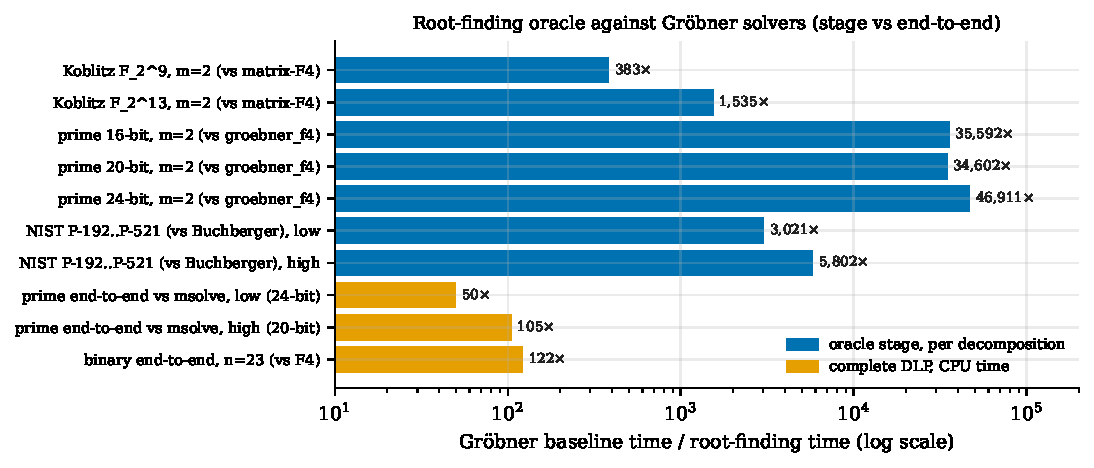
\includegraphics[width=\linewidth]{figures/fig-rootfind-oracle.pdf}
\caption[]{Root finding against Gr\"obner solvers on identical targets. Blue:
one decomposition (oracle stage only). Orange: complete discrete-log
computations with the oracle swapped and everything else fixed (prime: CPU
time against msolve, 20/24-bit totals composed from sampled per-query cost;
binary: one cold solve including table build). Sources:
\art{RESEARCH_SEMAEV_ROOTFIND_VS_GROEBNER.md},
\art{papers/rootfinding-decomposition/README.md}.}
\label{fig:rf-oracle}
\end{figure}

\paragraph{Oracle stage.} Per decomposition, root finding is
$383\times$ ($\FF_{2^9}$, $\abs\Fb=55$, 254 targets) and $1{,}535\times$
($\FF_{2^{13}}$, $\abs\Fb=4{,}005$, 256 targets) faster than matrix F4;
$3.5$--$4.7\cdot10^4\times$ faster than \texttt{groebner\_f4} on 16--24-bit
prime curves ($\abs\Fb=6$, 40 targets each); and $3{,}021$--$5{,}802\times$
faster than Buchberger on the decomposition ideal of the five NIST curves
(Figure~\ref{fig:rf-oracle}). Every binary verdict agreed with F4; every
prime solution was in F4's variety and every prime refutation was F4's unit
ideal. In the PDP study, \texttt{rf-mitm} refutes a binary target in
$3.1\,\mu$s at $\ell=8$ and $482\,\mu$s at $\ell=14$, against the PS-0
baseline's $9.3$\,ms and $55.5$\,s ($3{,}007$--$115{,}160\times$), costs
$5\abs\Fb-3$ multiplications and $2\abs\Fb$ lookups a target, and sits on
the pair-table floor at $1.000\pm0.027$ bits per rung; at prime $m=3$,
$N=18$ it uses 197 multiplications where F4 uses $8.99\cdot10^{13}$
multiply-adds; 707/707 brute-force agreements
(\art{research/pdp_root_finder_20261012/}).

\paragraph{Complete solves.} End to end, the gain is two orders of
magnitude smaller and not one-sided: $50$--$105\times$ against msolve on
16--24-bit prime curves; $122\times$ on the one binary instance ($n=23$)
large enough to amortise the pair table; and F4 \emph{faster} at
$n=5,9,13$, where a solve needs too few decompositions to pay for the
table. Inside ecbench, with every group operation charged, the
root-finding IC beats inherited F4 in solve wall by about $350\times$ at
$n=13$ (admitted) and about $10^4\times$ at $n=23$ (descriptive), yet stays
$2.9$--$25{,}116\times$ the strong rho in $S$ on binary curves and
$29$--$141\times$ rho on prime curves, with the gap widening
(\art{research/pdp_root_finder_ecbench_20261013/}).

\paragraph{The Koblitz loops.} Figure~\ref{fig:k13} follows the best
complete-count root-finding arm at Koblitz $E_0$, $n=13$ through four
registered improvement loops (8 public targets $\times$ 3 rounds each, L0
operation counts). The first engine had $S=38.82$ ($m=3$) and $28.38$
($m=2$). A windowed third-summand scan cut $m=3$ by a paired $0.828$
$[0.783,0.863]$; a fold over negation (\texttt{rootfind-negfold}) took
$m=2$ to $23.22$ and then $22.97$. Two further cycles of denser and
sparser bases, windowed negfold and plain root finding were dead ends
(\art{research/ecbench_rootfind_vs_rho_20261014/}). With F4's word XORs
priced, the paired ratio negfold/F4 is $0.0545$ $[0.047,0.064]$, a
complete-against-complete comparison; against strong signed-Frobenius rho
($S=14.82$) the best complete arm is still $1.55\times$. A compact-orbit
base with a counted Frobenius pair table reaches $S=15.55$, below the
then-unpriced F4 ($16.75$), but it is itself a lower bound
(factor-base construction natives unpriced), and it is $1.08\times$ rho.
Amortised over 64 targets that arm reaches $S\approx11.2$, below rho; by
the ledger's rules that is a secondary, multi-target result, not a cold
claim.

\begin{figure}[t]
\centering
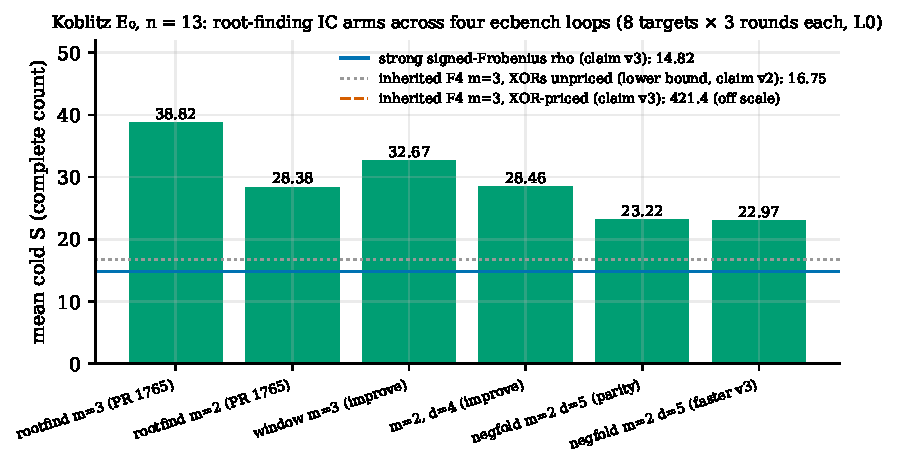
\includegraphics[width=\linewidth]{figures/fig-k13-progression.pdf}
\caption[]{Mean cold $S$ of root-finding IC arms at Koblitz $E_0$, $n=13$,
$d=5$ unless stated, across the engine, improve, parity and faster loops.
All bars are complete counts. Sources:
\art{research/ecbench_rootfind_engine_20261012/},
\art{research/ecbench_rootfind_improve_20261013/},
\art{research/ecbench_rootfind_parity_20261013/},
\art{research/ecbench_rootfind_faster_20261014/}. Each loop had its own
seeds and rho arm (rho $14.12$--$14.82$).}
\label{fig:k13}
\end{figure}

\paragraph{Prime tuning in ecbench.} On a 20-bit prime curve, the pair
table's counted $S$ is $0.018861$ $[0.018547,0.019242]$ of direct
subtraction (24 pairs; prime native work unpriced, so a bounded ratio), and
$0.057047$ $[0.041159,0.092069]$ on a 17-bit Koblitz curve, fully priced,
where the table set-up is about 68\% of the arm's cold cost. Doubling the
table from 32 to 64 abscissae gives $0.830$ $[0.697,0.962]$; three
summands instead of two costs $1.431\times$ $[1.225,1.716]$; batching the
table inversions leaves counted GAE unchanged ($1.000$; $4{,}096$ versus
$64$ inversions, set-up wall $243$ versus $128\,\mu$s, descriptive); and a
train-set lane selection did not resolve a hold-out winner ($0.979$
$[0.919,1.038]$; 1{,}088/1{,}088 verified executions)
(\art{benchmarks/README.md}, rows of 12--14 Oct).

\paragraph{Dense root index at $n=83$.} Widening the prefix base from
K1500 to K1798 cut mean probes per relation from $300{,}021.9$ to
$169{,}069.8$ (paired difference $130{,}952$, 95\% $[52{,}058,209{,}991]$)
and gave a one-point online ratio of $18.528$ over same-point rho (IC
$63.3$\,ms, rho $1{,}173.3$\,ms), with $339.0$\,s of reusable preparation
and an 8\,GiB table outside the window. The host was shared, so the result
is exploratory; two K1500 runs hit the 900\,s timeout and are retained.
The probe reduction stands; the online ratio does not: it was taken
against rho with an empty table, and rho with a precomputed table matched
to the index calculus's set-up is faster in every matched $n=83$ pair
(validation sweep, 20 October; \S\ref{sec:ladder2}).

\paragraph{Reading.} Root finding is the largest constant-factor change
of the programme at the oracle stage, and the one with a proof behind it.
It does not change the asymptotic count of index calculus: its cost is
$\Theta(\abs\Fb^{m-1})$, every measurement is at $m\le4$, and it leaves
relation yield, factor-base size and linear algebra untouched. Its effect
on the cold frontier is to move the decomposition stage from dominant to
minor, which exposes the stages that now are.

\chapter{Gr\"obner-basis engines}\label{sec:groebner}

Before root finding, the decomposition oracle was a Gr\"obner solve, and
for $m\ge3$ over binary fields it still is. The repository grew a family
of engines (\art{docs/ic/GROEBNER_F4F5F6_AUDIT_20261010.md}, \S1; file names below are under \art{src/cryptanalysis/}):

\begin{description}[style=nextline, leftmargin=1.4em]
\item[Matrix F4 and F5 over $\FF_2$] (\art{koblitz_groebner.rs},
  \art{matrix_f5_f2.rs}): Macaulay matrices of the Weil-restricted Boolean
  system, reduced by a shared Four-Russians kernel (\art{gf2_elim.rs}, four
  8-bit tables, AVX-512 or AVX2).
\item[Inherited F4] (\art{inherited_f4.rs}, from 22 September, the
  default algebraic oracle): a DPLL-style tree over partial assignments in
  which each child \emph{inherits} its parent's echelon form and re-reduces
  only what the assignment changed, instead of building a fresh Macaulay
  matrix per node.
\item[F6-IC] (opt-in): inherited F4 plus a factor-base domain gate (a
  fully assigned summand whose abscissa is not a base point refutes;
  partial support pruning refutes earlier), and meet-in-the-middle leaves
  (with $m-1$ summands fixed the last is looked up; at $m=3$ and
  $\abs\Fb\le256$ every compatible second point is added and the third
  looked up).
\item[$\FF_p$ F4] (\art{f4_fp.rs}, \art{f4_fp_tower.rs},
  \art{sig_fp_tower.rs}): degree-bounded F4 with sparse-by-reducer then
  dense reduction, a Faug\`ere--Lachartre block for the Kummer-tower
  oracle, and a signature variant.
\end{description}

\paragraph{Correctness.} The audit pinned every engine against every
other and against brute force (88+15+9+14+13+12+21+6 passing library
tests in the touched modules), and found one soundness bug
(\S\ref{sec:corrections}, item 6), two contract defects and several latent
holes, all fixed with regression tests.

\paragraph{Engineering results.} Figure~\ref{fig:engine} collects the
headline ratios and Table~\ref{tab:prog_groebner-engineering} lists them
all; all are \cls{engineering} with identical outputs.

\begin{table}[p]
\centering\footnotesize
\begin{tabular}{@{}>{\raggedright\arraybackslash}p{0.27\linewidth}>{\raggedright\arraybackslash}p{0.2\linewidth}>{\raggedright\arraybackslash}p{0.2\linewidth}>{\raggedleft\arraybackslash}p{0.2\linewidth}@{}}
\toprule
Change & Case & Measure & Ratio or value \\
\midrule
Matrix / inherited F4 & K13 & counted matrix work & $198.6\times$ \\
 & random-13 & & $222.1\times$ \\
 & $m=19$ & wall, matrix F4/F5 vs inherited F4 & timed out at 1{,}800\,s vs about 6\,s \\
\addlinespace
F5 / F4 & K13 & word XORs & $0.6465$ \\
 & random-13 & & $0.6414$ \\
 & K13, random-13 & wall & $0.79$--$0.86$ \\
\addlinespace
F6-IC / inherited F4 & $m=13$ & word XORs & about $0.82$ \\
 & $m=19$ & & $0.77$--$0.78$ \\
 & --- & relation wall & $1.7$--$1.9\times$ faster \\
 & $m=13$ & $S$, group additions charged & $64.6$--$68.8\times$ \\
 & $m=19$ & & $1{,}303$--$1{,}353\times$ \\
 & K13 & $S$, word XORs priced (\#1774) & $1{,}572.1/634.12\approx2.5\times$ \\
 & R13, $m=19$ & & lower bounds \\
 & $m=31$ & first target & both hit 3{,}600\,s cap \\
\addlinespace
Every echelon call to the Four-Russians kernel & oracle's own Macaulay matrices & speed-up & $1.75$--$3.22\times$ \\
Word-level \texttt{pext}/\texttt{pdep} rewrite plan & $n=23$ & F4 and F6-IC faster & 10--14\% \\
Eager / lazy rewrite of kept rows & & speed-up & $1.40$--$1.62\times$ \\
\addlinespace
Fused construction and readback & F4 & instructions & $-5.28\%$ \\
 & F5 & & $-11.02\%$ \\
Native hashing & F5 & & $-3.715\%$ $[3.714,3.726]$ \\
 & standalone criterion & & $-45.1\%$ \\
Bounded direct indexing in the F5 packer & F5 & & $-3.947\%$ \\
Row allocation & & requested bytes & $42$--$50\%$ fewer \\
\addlinespace
Quotient-curve model / symmetrised control & $m=2$, five interleaved cells & F4 word operations cut & $1.340$--$1.642\times$ \\
\addlinespace
Branchless AVX2 strip & one thread & speed-up & $1.210\times$ \\
Bitmap seen-set in Boolean F4 & full F4 & & $1.199\times$ \\
Combined F5 options & & & $1.530\times$ \\
Fixed support cut & one complete call & & $3.02$--$3.07\times$ \\
Graded reuse in F5 & & & $1.78$--$1.84\times$ \\
\addlinespace
\texttt{f4\_fp} / its predecessor & square generic systems & speed-up & $29.8$--$54.1\times$ \\
msolve / ours & single-threaded & ratio & $0.96$--$1.22$ \\
Ours / msolve, blocked pair reduction & two largest square systems & time & $0.75$--$0.78\times$ \\
 & four others & & $1.11$--$1.49\times$ \\
msolve faster, a day earlier & & time & $12$--$24\times$ \\
Boolean decomposition systems, $n=17$, 8 targets & our oracle (decides) & time per target & 7--24\,ms \\
 & msolve, PolyBoRi (full basis) & & 40--52\,s \\
 & Singular & & exceeds 120\,s \\
\bottomrule
\end{tabular}
\caption[]{Gr\"obner-engine engineering results, all \cls{engineering}
with identical outputs. \emph{Change}: candidate / baseline where a slash
is shown; \emph{Case}: target set or size (K13, random-13 and R13 as named
in the sources; $m$ the number of summands; ``---'': no
case given); \emph{Measure}: the counted or timed quantity; \emph{Ratio or
value}: as recorded. Groups, top to bottom, with sources: inherited versus
matrix F4 (\art{research/f4_f5_f6_cross_family_20261011/}); F5 versus F4;
F6-IC versus inherited F4 (priced and lower-bound cells:
\art{research/f4_pricing_jump_20261018/}); kernel routing and rewrite
(\art{research/inherited_f4_eager_rewrite_20261011/}); instruction and
allocation work, by paired A/B/A$'$ instruction counts on a frozen
eleven-system suite, elapsed time not claimed; the quotient-curve model
(\art{research/lit2026_w8_summation_models_20261011/}); $\FF_2$ campaign
results (strip: \art{research/gf2_branchless_strip_20260929/}; seen-set:
\art{research/boolean_f4_bitmap_20260926/}; combined options:
\art{research/f5_combined_2x_20260928/}; support cut:
\art{research/f5_support_cut19_confirm_20261003/}; graded reuse:
\art{research/boolean_f5_graded_batch_20261002/}); $\FF_p$ F4 to msolve
parity (\art{research/f4_fp_msolve_parity_20261011/}; blocked pairs:
\art{research/f4_fp_blocked_pairs_20261016/}; the day-earlier msolve
reading: \art{research/gb_cas_comparison_20261011/}).}
\label{tab:prog_groebner-engineering}
\end{table}

Matrix and inherited F4 can return different decompositions, so their
splitting trees may differ; only matrix F4 and F5 share a tree by
construction. F6-IC's $S$ ratios, once its batched group additions are
charged, are an accounting loss, not a frontier move. Those ratios used
inherited F4 before its word XORs were priced (\#1774); priced, F6-IC is
still a loss at K13, while the R13 and $m=19$ cells remain lower bounds.

The $\FF_2$ engine campaigns (about 90 directories, 22 September--17
October; the programme record~\cite{icprogram2026}, clusters ``boolean'',
``gf2-elim'', ``f5-kernel'', ``f5-support-cut'', ``f4-f5-shared'') gated
each micro-change against the strongest reference, and most failed. Kept as
defaults: the branchless strip, the bitmap seen-set, batched pair inserts,
five-column tables, and direct packing in F5 (default since 17 October).
About thirty unpack, pivot, layout and packing variants were refuted, and
graded reuse in F5 fell short of the campaign's $2\times$ goal. These are
stage speed-ups of the decision engine; none changes an index-calculus
distance to rho. Every reduced basis of \texttt{f4\_fp}, after
Gebauer--M\"oller criteria, packed monomials, interned symbolic
preprocessing and a parallel symbolic pass, agrees with Singular or msolve.
The Boolean comparison is a difference of task (decide versus compute the
basis), not of engine quality.

\begin{figure}[t]
\centering
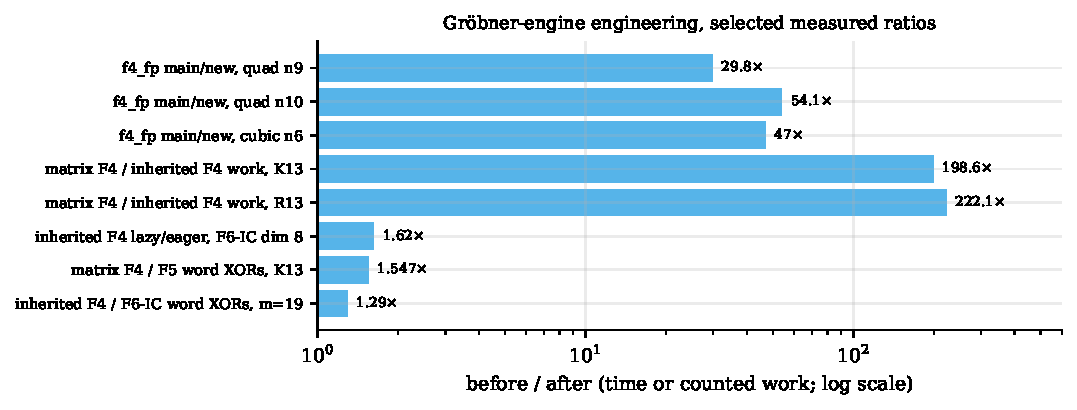
\includegraphics[width=\linewidth]{figures/fig-engine.pdf}
\caption[]{Selected engine ratios (before/after or baseline/candidate):
\texttt{f4\_fp} successive versions (single-threaded wall, L0); matrix
versus inherited F4 (counted matrix work); lazy versus eager inherited
rewrite (median wall); F4 versus F5 and inherited F4 versus F6-IC (word
XORs, stage only). Sources in \art{figures/data-program.json}.}
\label{fig:engine}
\end{figure}

\paragraph{What did not work.} Degree-2 early-abort probes after a
2025--26 proposal: word-XOR ratios $1.00083$--$1.00378$ (no change) and
$0.99714$--$0.99928$ (worse). Gate-first geometry: $1.57$--$1.78\times$
fewer word XORs but lane-batched F4 roots cost $2.6$--$4.0\times$ a
sequential control. Convolution splitting of the summation polynomial:
$1.21$--$2.07\times$ \emph{more} word operations despite lower degree;
Frobenius auxiliary variables: $57$--$701\times$ more
(\art{research/lit2026_w\{4,5,8\}_*_20261011/}). Symmetry-breaking clauses
in SAT did not help (\art{RESEARCH_KOBLITZ_INDEX_CALCULUS.md}). A
registered law for the $m=3$ refutation degree resolved all 68 units but
ended with the verdict ``neither'': one variant met its generic degree
window on 32/32 draws, the other fell below it on 8, and the heaviest
degree-10 Macaulay solves were $2.4\cdot10^5\times2.0\cdot10^5$ matrices at
42--51 minutes each (\art{research/ic_semiregular_law_20261005/}).

\chapter{Koblitz curves}\label{sec:koblitz}

Koblitz curves $E_a: y^2+xy=x^3+ax^2+1$ over $\FF_{2^n}$, $a\in\{0,1\}$, carry
the Frobenius endomorphism $\tau$, which acts on the prime-order subgroup as
a known scalar $\lambda$; ECC2K-130 is the $a=0$, $n=131$ member. They were
the programme's main family: the compact-orbit producer, the $n=83$
campaign, leaderboard Table~A and the ECC2K-130 cost model all live here.
Random and prime-degree binary curves without $\tau$ are in
\S\ref{sec:binary}, and the Weil-descent degree studies that price
ECC2K-130's algebraic route are there too, because their systems use random
subspaces rather than Frobenius structure. Every study in this section is
listed in the programme record~\cite{icprogram2026}.

\section{Frobenius-invariant and compact-orbit bases}

The Koblitz implementation (\art{src/cryptanalysis/koblitz_index_calculus.rs})
builds GGMP's invariant base from the linearised polynomial of a factor of
$x^n-1$, checks $\pi(\Fb)=\Fb$ point by point, rewrites each relation into
orbit columns with known $\lambda^k$ weights, and solves the
cofactor-corrected system $h a+hbd\equiv\sum\lambda^{k_i}x_{o_i}$. On
small fields the orbit collapse is as predicted: $\abs\Fb/\#\text{orbits}$
of $7.86$, $10.89$, $12.96$ at $n=9,11,13$ for relations and
$61.7$--$168.0$ for linear algebra, against rho's $4.24$--$5.10$
(\art{RESEARCH_KOBLITZ_INDEX_CALCULUS.md}). Because $\ell=\operatorname{ord}_n(2)$
fixes the invariant base's size, the programme moved to bases sized to the
instance: divisor bases, SAT-optimised bases, a rank-guided base at $n=53$
(220 orbits, a complete implicit $\Sem5$ formula of 22{,}887 clauses), and
finally the \emph{compact signed-Frobenius orbit} base, which stores one
representative per orbit and no pair table
(\art{docs/ic/COMPACT_ORBIT_PRODUCER.md}). In the ecbench factor-base
suite it is the best measured Koblitz construction: $S=9.114$ at $n=17$
($272$ points, 8 columns), $9.985\times$ matched signed-Frobenius rho,
against full orbit $18.7\times$ and subspace bases $47\times$
(\art{research/ecbench_frontier_20261013/}).

\section{The oracle sequence}

The binary oracle went through SAT (XOR-native CDCL after Trimoska et
al.~\cite{trimoska2020}; decides the $n=19$, $\ell=6$ corpus but does not
scale), matrix F4 (whose refutation range was the real frontier),
pairs-and-solve for $\Sem4$ (validated to $n=21$, $\ell=7$, still
$O(2^{2\ell})$), meet-in-the-middle pair tables, inherited F4 and F6-IC
(\S\ref{sec:groebner}), and root-finding engines (\S\ref{sec:rootfinding}).
The boundary ledger's current Koblitz decomposition record is an $n=31$,
$m=2$ F4 cell with an exact block-6 M4RI acceleration; at $n=53$ an exact
Frobenius-orbit $\Sem5$ compression removes the coordinate ROM but every
unrestricted solver arm remains \textsc{unknown}.

The September toy studies that fed this sequence are catalogued as
campaigns. At $n=13$ and $n=19$, rotated subspace bases covered $1{,}591$ of
$2{,}003$ targets with five spaces against $61$ with one, and joint rank
recovered $58/64$ targets against $29/64$, without passing a 10\% yield
gate at $n=19$ (\art{research/notes/ecc2k130/}, clusters
``rotated-n13'' and ``rotated-n19''). Finite-fibre $\Sem3$ semantics were
proved exact and an $O$-aware CNF made $252.7\times$ smaller at $n=13$, but
no existing solver interface was admitted as an arm; three SAT engines
decided 5 satisfiable and 27 unsatisfiable targets at $n=13$, with the five
negatives DRAT-certified. At $n=131$ a symbolic full-point DAG replayed a
single-edge DIMACS instance but could not be admitted past the 64-bit
ceiling, and the exact Frobenius census of the balanced $(m,d)=(10,13)$
rotated base has $1{,}048{,}134$ columns, the only shape with as many columns
as the field. A frozen test of the Frobenius quotient found that toy fields
saturate and so test nothing; an independent SAT reproduction solved
$n=13$ and none of four planted targets at $n=19$ in 1{,}200\,s
(\art{research/frobenius_quotient_sat_20260930/}). At $n=13$ the
presentation of the curve does not matter: yield spread is explained by
cofactor balance (correlation $0.850$) and there is no curve effect at
$n=19$ (intraclass correlation $\le0.006$;
\art{research/koblitz-isogeny/}).

\section{Against a stronger rho: the September reversals}\label{sec:koblitz-strong}

Three September results that put Koblitz index calculus at or below rho
were reversed when rho was strengthened, which is why every later row is
quoted against the strongest available rho
(\S\ref{sec:corrections}). Table~\ref{tab:prog_koblitz-reversals} gives
each result as recorded and against the stronger rho.

\begin{table}[t]
\centering\small
\begin{tabular}{@{}llllr@{}}
\toprule
Result & Case & Measure & Recorded & Stronger rho \\
\midrule
Tournament & $n=43$, $a=1$, best & retired instr. & $0.5347$ & \\
 & $n=43$, $a=1$, triple table & & $0.409$ & \\
 & five cells$^{e}$ & & & $1.19$--$2.88\times$ \\
\addlinespace
Orbit DLP & $n=53$, 1{,}024 targets & retired instr. & $0.2403$ & \\
 & four rungs & & & $0.240\to0.317\to1.294\to1.923$ \\
 & sweep, $n=37$ & & & $0.794$ \\
 & sweep, $n=41$ & & & $1.520$ \\
 & sweep, $n=53$ & & & $1.923$ \\
 & sweep, $n=61$ & & & $2.297$ \\
 & single target & & $0.8392$$^{a}$ & $44.0\times$ $[39.4,45.4]$ \\
\addlinespace
Compact orbit & $n=41$, $L=1{,}024$ & corrected rho & $0.309\times$ & \\
 & $n=37$, $L=1{,}024$ & 32-walk rho$^{b}$ & & $2.081$ \\
 & $n=53$, $L=1{,}024$ & & & $3.086$ \\
 & $n=41$, $L=1{,}024$ & cold CPU$^{c}$ & & $1.314$ \\
 & $n=53$, $L=1$ & & & $22.675$ \\
 & $n=37$, $L=1{,}024$ & instructions$^{d}$ & & $0.5165\times$ \\
 & $n=41$, $L=1{,}024$ & & & $0.6221\times$ \\
\bottomrule
\end{tabular}
\caption[]{IC/rho of the three September results as first recorded and
against a strengthened rho. Tournament (15 September): IC against a worker
rho's retired instructions; giving rho the index calculus's own canonical
form made rho win all five cells
(\art{research/ic_triple_counted_20260923/}; the tournament README,
\art{research/ic_candidate_tournament_20260915/}, carries no correction
note). Orbit DLP: the recorded rho used software carry-less multiplication
on x86-64; rho was strengthened in four rungs, then the preregistered sweep
read rising with $n$
(\art{research/notes/index-calculus/RESEARCH_STRONG_RHO_LADDER_20260929.md});
$^{a}$the selected-panel crossover withdrawn by the direct arm's cost
against a strong single-target rho
(\art{research/notes/index-calculus/RESEARCH_SINGLE_TARGET_STRONG_RHO_N53_20260930.md}).
Compact orbit: the recorded value is a point panel;
$^{b}$a 32-walk batched-inversion normal-basis rho
(\art{research/notes/ecc2k130/compact_orbit_strong_rho_20260929/RESULT.md});
$^{c}$compact/rho CPU of the orbit-disjoint cold confirmation, which ended
with six eligible no-gos
(\art{research/notes/ecc2k130/disjoint_cold_v2_outcome_20261001/RESULT.md});
$^{d}$batched compact IC
(\art{research/notes/ecc2k130/compact_ir_ledger_20260930/RESULT.md}).
$^{e}$Rho given the index calculus's own canonical form.}
\label{tab:prog_koblitz-reversals}
\end{table}

Batched compact IC does use fewer instructions than rho while its cold CPU
stays above rho, a gap traced to memory behaviour. Some sixty notes on S3
batch inversion, swap quotients, Bloom prefilters, window screens and $K$
grids each moved a constant and none crossed rho (cluster
``compact-orbit-cold'').
The boundary ledger of the same weeks reached the same place from the other
side. Re-pricing every row against a matched negation rho raised the vs-rho
ratios $2.1$--$6.5\times$ (\art{research/ic_rho_reference_20260923/}); the
best batch row was $4.86\times$ $[4.21,5.55]$ at $r=2^{39}$, and a page
$r^{1/6}$ law was falsified at the small end
(\art{research/ic_exponent_20260926/}); single-target online IC beat
table-less rho at all six sizes ($8.84$--$17.5\times$) while cold rho won at
all six ($1.98$--$31.6\times$; \art{research/ic_single_target_20260930/}).
At $n=37$ in ecbench the cold IC/rho was $3.64\times$ in instructions and
$13.6\times$ $[10.6,18.7]$ in counted $S$, and the $n=37$ parameters did not
transfer to $n=41$ or $n=53$
(\art{research/ecbench_n37_shared_rank_20261004/},
\art{research/ecbench_n41_n53_shared_rank_20261005/}). An $m=4$ exponent
audit measured a cost slope of $0.985$--$1.060$ bits per unit of $n$ at
$n\le19$, against the $0.25$ the lead needed
(\art{research/ic_m4_exponent_audit_20260928/}).

\paragraph{Other Koblitz lines.} The remaining Koblitz campaigns moved
constants inside index calculus and are catalogued in
the programme record~\cite{icprogram2026}. Instruction-level rounds on the Gröbner stage
left the whole relation log at $964\times$ rho on $K_0$ over $\FF_{2^{13}}$
(\art{research/groebner_instructions_20260925/}); a September autolab
campaign cut cold instructions by $47.7\%$ and left the candidate at
$4.98\times$ matched rho's instructions (\art{research/ic_autolab_next30_20260915/});
at $n=37$ a full-rank compact-orbit gate passed with IC at $22.6\times$ rho
(\art{research/notes/ecc2k130/full_rank_compact_orbit_ic_20261003/RESULT.md}).
Pipeline kernels gave laned canonical keys $1.09$--$1.31\times$
(\art{research/canon_laned_keys_20261008/}), u64 root batching
$3.26\times$ whole-process wall (rank cell corrected to $2.47\times$), and
aimed gathering $1.037\times$ set-up (\art{research/ic_aimed_gather_20261023/}).
Transporting a base through ECC2K-130's degree-263 and degree-7 isogenies
was built and certified, but on toy fields the transported and descendant
bases cost $3.6$--$4.0\times$ the original
(\art{research/ecc2k130_factor_base_pilot_20260924/}); and $\tau$-adic
known-scalar arithmetic is $0.413$ of the binary cost at $m=131$ with no
measured rho benefit
(\art{research/notes/ecc2k130/tau_adic_arithmetic_20260929/README.md}).
On the rho side, GPU iteration redesigns for the ECC2K-130 walk did not
beat the shipping distinguished-point walk
(\art{research/ecc2k130_iteration_redesign_20261012/},
\art{research/dp32_sigma_table_20261012/}).

\section{The one-target online ladder}

The ledger's primary \texttt{vs\_rho} question is: with reusable IC
preparation already done, how long does one unseen public target take,
against rho with the automorphism discount on the same point? The ladder
(Figure~\ref{fig:online}) is in Table~\ref{tab:prog_koblitz-ladder}.

\begin{table}[t]
\centering\small
\begin{tabular}{@{}rlrrlrl@{}}
\toprule
$n$ & Base & Columns & Points & Memory & Rho/IC online & Status \\
\midrule
53 & shared-log$^{a}$ & & & 9.34\,GB & & \\
61 & compact orbit & 600 & 73{,}200 & 2.73\,GB & $124.85\times$ & exploratory$^{b}$ \\
71 & & & 85{,}200 & & $2{,}864.1\times$ & exploratory$^{c}$ \\
73 & & & 87{,}600 & & $1{,}189.7\times$ & exploratory$^{d}$ \\
83 & $a=1$ & & & & $8.2\times$ & exploratory$^{e}$ \\
\addlinespace
\textbf{61} & orbit, $a=0$ & $K=500$ & $61{,}000$ & & $13.94\times$ $[9.81,19.13]$ & admitted$^{f}$ \\
 & & & & & $12.87\times$ $[7.30,19.08]$ & admitted$^{g}$ \\
\bottomrule
\end{tabular}
\caption[]{The one-target online ladder: rho online time over IC online
time on the same point, reusable IC preparation excluded; peak memory where
recorded (peak RSS at $n=53$). $^{a}$Guided shared-log precompute with an
explicit pair table; earlier, a 1{,}024-target shared-log batch beat batched rho
in all 15 paired blocks (secondary, multi-target). $^{b}$Fresh
reproduction. $^{c}$First rung past 64-bit packing (u128 words); median of three
repeats of one point. $^{d}$The guided-rank precompute took 5.1\,h at
57--70 million probes per relation. $^{e}$IC online 5.6--7.9\,s against
rho 43--71\,s; re-measured below. $^{f}$Admitted 12 October: 64 fresh
public one-target workloads per host, identical candidate manifest on two
hosts; median online speed-up with 95\% interval; pinned x86\_64,
claim-check 64/64. $^{g}$The same, unpinned arm64.}
\label{tab:prog_koblitz-ladder}
\end{table}

Re-measured on 12 October against a default strong rho on five repeats of
the same target, the $n=83$, $a=1$ IC was \emph{slower} online,
$1.382\times$ $[1.036,1.882]$, and $218.0\times$ rho in fresh-process wall
time (\art{research/n83_evaluation_20261012/}); the later dense-root
reading of $18.5\times$ is in \S\ref{sec:n83}. For the admitted $n=61$
point, set-up of about 28\,s is outside the window; with it charged, IC
costs a median $83.4\times$ rho.

\begin{figure}[t]
\centering
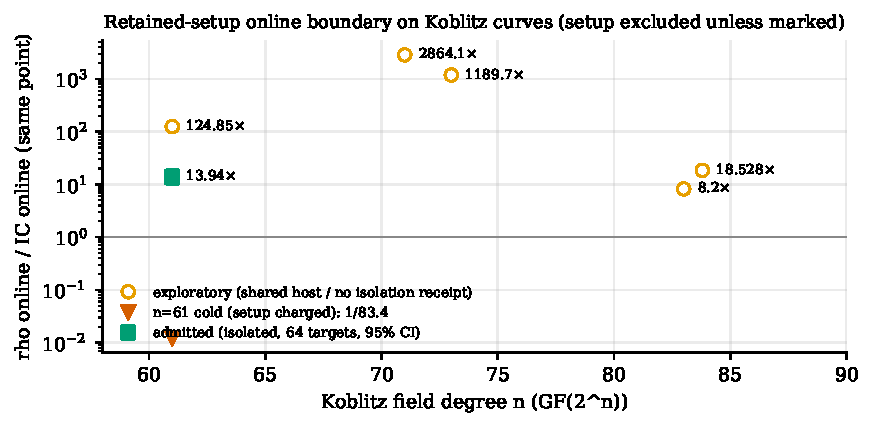
\includegraphics[width=\linewidth]{figures/fig-koblitz-online.pdf}
\caption[]{Rho online time over IC online time on the identical public point,
reusable IC preparation excluded. Open circles: exploratory (verified
answers, no qualifying isolation receipt; three repeats of one point or a
single point). Filled square: the admitted 64-workload panel with its 95\%
bootstrap interval. Triangle: the same $n=61$ candidate with set-up
charged (cold). Sources: \art{docs/ic/boundary_targets.json},
\art{docs/ic/PLAN_IC_ACCOUNTING_FIXES_20261007.md},
\art{research/n83_dense_root_20261013/}.}
\label{fig:online}
\end{figure}

The exploratory ratios are large and irregular because a one-point online
window measures the luck of one relation search against one rho walk; the
admitted panel's range over 64 workloads is $1.06$--$648.6\times$. The
admitted point is a constant-factor online result at $n=61$ (47-bit
subgroup) with preparation retained; it is not a cold result, not a
scaling law, and not an asymptotic claim.

\emph{Retired as an index-calculus win (14 October).} Every rung of this
ladder compares index calculus with a retained table against rho with
none. Given a distinguished-point table of equal or smaller size,
Bernstein--Lange preprocessing rho~\cite{bl2012} is $53$--$317\times$
faster online than the compact-orbit arm on the same 64 targets at $n=41$,
53 and 61 (\S\ref{sec:ladder}). At $n=83$ (\S\ref{sec:n83}) rho with a
table matched to the index calculus's set-up time or memory won every pair
that was run. The ladder therefore measures what a table buys, and generic
rho buys more per byte. The validation sweep later found
\art{docs/ic/BOUNDARY_TARGETS.md} still printing the $13.94\times$ as a
win; it is superseded
(\art{research/validation_sweep_20261019/B-benchmarks/VERDICT_TABLE.md}).

\section{The $n=83$ campaign}\label{sec:n83}

Degree 83 was the programme's largest Koblitz target with a working
pipeline: 145 study directories between 4 and 21 October
(the programme record~\cite{icprogram2026}, clusters beginning ``n83'' and ``f6-n83'').
In order:
\begin{itemize}
\item \emph{F6 micro-studies, 4--5 October} (24 directories, almost all on
  the $a=0$ curve). They kept kernel gains (queries up to $2.998\times$
  faster, resident memory $-52\%$) and shrank SAT encodings, but every
  ordinary solve timed out; four-summand coverage was at most
  $4.662\cdot10^{-12}$ of the subgroup and no natural relation was found.
  On the 81-bit $a=0$ gate curve, SAT and XCNF decompositions succeed only
  with a known witness, and the prebuilt-base question is an open problem
  record.
\item \emph{The $a=1$ point, 7--12 October.} The archived K600 point read
  $8.2\times$ online and was re-measured slower (above).
\item \emph{Root-index capacity, 13--16 October} (25 directories). Root-index
  layouts grew the $a=1$ base from K512 ($84{,}992$ points) to K3596
  ($596{,}936$ points) within 14\,GiB. The dense root index cut probes per
  relation from $300{,}021.9$ to $169{,}069.8$ (K1500 to K1798; paired
  difference $130{,}952$ $[52{,}058,209{,}990]$), a within-IC result that
  stands; its one-point online $18.528\times$ is retired
  (\art{research/n83_dense_root_20261013/}).
\item \emph{Factor-base selection, 14--16 October} (56 directories). Root4,
  root11 and root21 layouts, Bloom filters, sparse and canonical variants
  and $K$ screens from 100 to 20{,}000 points selected within index calculus;
  the best means are about 26--29\,ms online (K3425, K3450, K3500), and
  many screens end \textsc{bounded\_unknown}. A three-hash 512\,MiB Bloom
  filter cut a K3300 online mean from $34.77$ to $31.32$\,ms
  (\art{research/n83_root11_bloom_results_20261015/}); a K3350 win of
  $7.18\%$ did not replicate.
\item \emph{Tier-1 online readings, 14--16 October} (14 directories): median
  rho/IC of $54.1$, $210.3$, $113.0$, $104.2$, $35.1$, $413.3$ (one point)
  and $208.7\times$ (K3072, five fresh points, $[38.3,2{,}510]$;
  \art{research/n83_tier1_online_20261016/}), all against a rho with no
  table and with set-up excluded.
\item \emph{The control, 16 October.} Bernstein--Lange rho given a
  distinguished-point table matched to the index calculus's set-up time or
  memory was faster online in every pair run: IC/rho $3.74$
  $[2.65,11.05]$ (K3300, time-matched), $40.61$ (K3300, memory-matched),
  and $81.5$--$395.5$ (K600)
  (\art{research/20261016-n83-precomputed-rho-control/}). Only the K3300 and
  K600 bases were paired; the K3072 reading was not, so its retirement rests
  on the same mechanism rather than on its own measurement. The validation
  sweep and the ledger audit retired all the online readings on 19--20
  October.
\item \emph{Cold, 16--21 October} (11 directories). The cold one-target
  process fell from about 150\,s (K1024) to $119.8$\,s (K1120, holdout) and
  $113.8$\,s (K1107; \art{research/n83_cold_base_confirm_20261021/}), against
  a rho online time of about 2.2--2.6\,s on the same hosts. No matched cold
  rho was run, so no cold ratio is admitted; the hosted single-target
  benchmark's $133.7\times$ is the nearest cold figure
  (\art{benchmarks/20261014-n71-n83-hosted-single-target/}).
\item \emph{A second pipeline in \texttt{cryptanalysis}} (K600, $a=1$;
  \cite{icprogram2026}). A Tier~1 ratchet of rank-probe, closure,
  index-build and rank-finder changes brought its latest row to $3.92\times$
  a tuned rho end to end, cold, and $0.093\times$ online with set-up
  excluded (\art{ca:experiments/koblitz-n83-rankfinder-20261021/README.md}).
  The study's own limits apply: one run on one host class, a point estimate
  with no interval, wall time, factor-base construction charged to no arm (so
  the cold cost is a lower bound), no computable band, and gaps that are not
  comparable across runs (the same producer read $4.42\times$ on another host).
  Against Bernstein--Lange rho with equal advice its online time is
  $22.55\times$ $[16.23,31.44]$ worse
  (\art{ca:experiments/koblitz-n83-bl-rankprobe-20261019/}). It is the
  closest cold Koblitz figure at $n=83$ and is still above rho; the two
  pipelines' numbers are not comparable with each other.
\end{itemize}
The open pull requests at the time of writing include further $n=83$ work
($m=4$ queries on a retained 16{,}627-column base, AWS replays, shared-binary
panels); none is on \texttt{main} (the programme record~\cite{icprogram2026}).

\section{Leaderboard Table A: the Koblitz rules}\label{sec:tablea}

Table~A of \art{docs/ic/LEADERBOARD.md} prices one unseen public target on
Koblitz curves at $n=41$--$61$ ($\log_2r=36.6$--$47.2$), cold, against rho on
the same point. Its history is a sequence of rules, each a pipeline baseline
plus a rho reference (\art{research/ic_tool_program/}).
Table~\ref{tab:prog_koblitz-tablea} lists the rules and the pipeline
baselines.

\begin{table}[t]
\centering\small
\begin{tabular}{@{}llr>{\raggedright\arraybackslash}p{0.3\linewidth}@{}}
\toprule
\multicolumn{4}{@{}l}{(a) Rules: cold IC/rho on one unseen public target} \\
\midrule
Rule & Date & IC/rho, cold & Status \\
\midrule
v3 & & $5.23$--$21\times$ & printed in Table~A; unvalidated (pre-gate) \\
v6 & & $3.78$--$12.06\times$ & rho reference $0.57$--$0.85$ of strong walk$^{a}$ \\
v7 & & $3.43$--$11.51\times$ & rho reference $0.57$--$0.85$ of strong walk$^{a}$ \\
v8 & 19 October & $4.67$ $[4.34,5.07]$ to $18.07$ $[15.98,20.58]\times$ & matched GFNI rho; archived as incomplete$^{b}$ \\
v4 recipe & 24 October & $9.9$--$43\times$ & validation file withheld$^{c}$ \\
\bottomrule
\addlinespace
\multicolumn{4}{@{}l}{(b) Pipeline baselines, 16--17 October: cold speed-up} \\
\midrule
Baseline & Change & Cheaper cold & \\
\midrule
v4 & head-of-main & & \\
v5 & scan-key & $1.20$--$1.24\times$ & \\
v6 & scan-fold & $1.33$--$1.40\times$ & \\
v7 & build streams & $1.07$--$1.13\times$ & \\
v8 & admitted prefetch & $1.06\times$ & \\
v4$\to$v8 & together & $1.90$--$1.98\times$ & \\
\bottomrule
\end{tabular}
\caption[]{Leaderboard Table~A, Koblitz $n=41$--$61$. (a)~Each rule's
cold IC/rho range over its sizes, against rho on the same point (rules v6
and v7: \art{benchmarks/20261016-ic-rule-v7/}; v8:
\art{benchmarks/20261019-ic-matched-rho-v8/}; v4 recipe:
\S\ref{sec:ladder3}). $^{a}$Per step, so the distance was understated.
$^{b}$$1.30$--$1.58\times$ the v7 control, fitted slope $0.168$ per $\ln r$;
its row is listed although the run is archived as incomplete. $^{c}$A paired
retuning improved one size of six; rho is priced in the same process at the
canonical batched step, and the validation file is withheld because that
reference may not be the strongest, so it is not an admitted row either.
(b)~Each baseline's recorded speed-up, and the combined cold factor over
v4 (\art{benchmarks/20261017-ic-r12-admitted-prefetch/}).}
\label{tab:prog_koblitz-tablea}
\end{table}

Under rules v6 and v7 cold rho was still faster at every size
(Table~\ref{tab:prog_koblitz-tablea}(a)). Seven further baseline candidates (prefetch gates,
filter slots, huge pages, a wider base) did not clear their rounds.
Table~C prices a 32-target batch on nine Koblitz curves ($\log_2 r=18$--$47.2$)
against batch rho on the same targets: $3.62$--$14.9\times$, a historical
diagnostic under the one-target rule. All nine failed the 24 October
validation gate, and Table~D, the Joux--Vitse historical study, is withheld.

The validation sweep found that Table~A understates its gap to rho by
$1.7$--$2.0\times$, and the 24 October validation gate did not check Table~A
(\art{research/ic_validation_gate_20261024/}). Rules v8 and v4 measure the
same sizes against differently built rho references and are kept apart
(Definition~\ref{def:domain}).

\section{ECC2K-130}\label{sec:ecc2k130}

ECC2K-130 is the $a=0$, $n=131$ member of the same family, with a 130-bit
prime subgroup and rho at about $2^{60.81}$ group operations. The compact
producer already solves $n=41,53,61,71,73$ of the family; about 300 notes
under \art{research/notes/ecc2k130/} price the routes to $n=131$ itself. No
route prices below rho.
Table~\ref{tab:prog_koblitz-ecc2k130} lists the priced algebraic routes.

\begin{table}[t]
\centering\small
\begin{tabular}{@{}llrr@{}}
\toprule
Route & Setting & Cost & Above rho \\
\midrule
Decomposition oracle & family bottom & $2^{132.58}$ & \\
 & Frobenius-orbit unions, $m=3$ & $2^{124.99}$ & $2^{64.18}$ times \\
\addlinespace
Relation sweep & best single relation, $m=4$ & & $+4.98$ bits \\
 & best honest $m=8$, Frobenius quotient & & $+13.59$ bits \\
\addlinespace
Linearisation & plain & & $70.19-b_{\max}$ bits \\
 & best bilinear XL, $\omega=2$ & & $71.82$ bits \\
 & same, $\omega=2.81$ & & $78.15$ bits \\
 & trilinear & & $87.16$ bits \\
\addlinespace
Weil descent & $m=3$, free oracle & $2^{68.58}$ & \\
 & $m=4$, degree 4 & $2^{68.43}$ & $+7.62$ bits$^{a}$ \\
 & $m=4$, degree 5, $w=1$ & $2^{71.13}$ & $+10.32$ bits \\
 & $m=4$, degree 5, $w=2$ & $2^{106.52}$ & $+45.71$ bits \\
 & $m=4$, hybrid guess & & $+8.43$ to $+58.27$ bits \\
\bottomrule
\end{tabular}
\caption[]{Priced algebraic routes to ECC2K-130. \emph{Setting}: the
variant priced ($m$ summands, $w$ as in the source, $\omega$ the
linear-algebra exponent); \emph{Cost}: the route's cost as recorded;
\emph{Above rho}: its distance to rho, as a factor or in bits. The
decomposition bottom needs a materialised base of $2^{44.53}$ points at
$m=3$; the $m=4$ single relation needs $2^{70.79}$ bytes; linearisation
gaps charge each Macaulay solve; the descent rows are in unconverted column
touches. $^{a}$Now contradicted. Sources:
\art{research/notes/ecc2k130/RESEARCH_ECC2K130_DECOMPOSITION_TARGETS.md},
\art{research/notes/ecc2k130/RESEARCH_ECC2K130_RELATION_SWEEPS.md},
\art{research/linearization_reach_20260930/},
\art{research/xl_bilinear_core_20261006/},
\art{research/xl_trilinear_t_unknown_20261006/},
\art{research/notes/ecc2k130/RESEARCH_ECC2K130_DESCENT_DEGREE.md}; the
hybrid guess is in \S\ref{sec:binary-descent}.}
\label{tab:prog_koblitz-ecc2k130}
\end{table}

\begin{itemize}
\item \emph{Extrapolating the producer.} The fitted probes-per-relation law
  $C\,r/(n^2K^2)$ with $C=1$ gives $1.1\cdot10^{18}$ core-years at $K=600$
  and $6.8\cdot10^{8}$ at $K=10^{12}$ columns
  (\art{RESEARCH_ECC2K130_IC_FEASIBILITY.md}, with the unexplained
  factor-of-5 gap in $C$ of \S\ref{sec:corrections}).
\item \emph{Decomposition oracles.} Decompositions exist, but no oracle
  finds one for less than $2^{131}$ per family; unions of Frobenius orbits
  lower the family's bottom but not to rho. Crossbred, RR-solver and WDSat
  oracles are engineering only: Crossbred is $0.023$ of F4's bit operations
  at $m=3$ but slower end to end, and the RR solvers' advantage over Semaev
  at $d=6$ is worthless against brute force.
\item \emph{Linearisation and Weil descent.} Neither reaches rho
  (Table~\ref{tab:prog_koblitz-ecc2k130}). The studies behind the descent
  rows, and the hybrid guess for the $m=4$ row, are in
  \S\ref{sec:binary-descent}.
\item \emph{Covers.} Over $\FF_{2^{131}}$ every ordinary curve has GHS
  magic number 1 or 131, so GHS descends ECC2K-130 to genus 1 (a zero map on
  the subgroup) or to genus about $2^{130}$, and the Hess--Menezes--Teske walk
  has nowhere to land. One question is open: $\langle G\rangle$ is the group
  of a simple 130-dimensional abelian variety, and if that variety were
  isogenous to a Jacobian with an evaluable isogeny, index calculus on the
  genus-130 curve would cost $2^{37.17}$, $2^{23.64}$ times \emph{less} than
  rho; no such curve is known, the Torelli codimension at genus 130 is
  8{,}128, CM constructions with prescribed Frobenius stop at genus 3, and the
  largest published Weil-descent discrete logarithm is at genus 31 over
  $\FF_{32}$ (\S\ref{sec:transfer})
  (\art{research/notes/ecc2k130/RESEARCH_ECC2K130_HYPERELLIPTIC.md}, with the
  magic-number correction of
  \art{docs/audits/GHS_MAGIC_NUMBER_MMT_CORRECTION_20261013.md}). The
  $N=130$ counterfactual is genus 255 at a modelled $2^{55.60}$ against rho's
  $2^{60.31}$, and measuring one relation trial turns that margin negative
  (\S\ref{sec:ladder3}). The best explicit curve construction reaches genus
  $2^{28.92}$
  (\art{research/notes/ecc2k130/RESEARCH_ECC2K130_CURVE_CONSTRUCTION.md}).
  The isogeny class has 262 curves of conductor gap 263 and no measured
  level effect (\S\ref{sec:transfer}); rho on the degree-263 leaves keeps
  only the negation map, an $11.45\times$ penalty
  (\art{research/notes/ecc2k130/isogeny_rho_speed_20260930/}).
\item \emph{Rho itself.} The separate GPU rho estimate is about 4.3 RTX PRO
  6000 card-years (\art{paper/ecc2k130/}); on one CPU core the ECC2K-130
  client walks 13.2 million steps per second
  (\art{research/certicom131_rho_ic_bench_20261022/}). Signed $\sigma$ steps
  cut modelled GPU time to $0.961$--$0.970$
  (\art{benchmarks/20261014-ecc2k130-signed-sigma/}).
\end{itemize}
Index calculus is not a route to ECC2K-130 on this evidence: every route
that has been constructed or priced is at least about 5 bits above rho (the
$m=4$ single-relation row, at $2^{70.79}$ bytes), most by tens of bits, and
the one hypothetical route below rho needs a genus-130 curve that no known
method can construct.

\section{Factor bases closed under $\ZZ[\tau]$}

The $\ZZ[\tau]$ small-norm multiplier base of 23 October
(\art{research/ic_improve_20261023/README.md}) is the latest Koblitz
change: $1.9$--$4.4\times$ child CPU at $n=41$--$61$ and $6.2$--$10.5\times$
at $n=71$, against the programme's own producer, exponent unchanged; it is
discussed with the other known-logarithm bases in \S\ref{sec:ladder3}.

\chapter{Random and prime-degree binary curves}\label{sec:binary}

This section covers binary curves $y^2+xy=x^3+ax^2+b$ over $\FF_{2^n}$
with $n$ prime, attacked with random subspace bases that use no Frobenius
structure, whether the curve is random or Koblitz: the Weil-descent route and the
degree question behind the subexponential claims
(\S\ref{sec:theory}), the decomposition oracles, the random-binary
leaderboard rows, and the 131-bit ECC2-131 target. Many of the descent
studies were priced for ECC2K-130 because it was the programme's named
target, but their systems are built on prime-degree fields with random
subspaces and use no Frobenius structure (the systems at $n=19,21$ say so
explicitly), so they belong here. The Gröbner and $\FF_2$ engines they run
on are in \S\ref{sec:groebner}; every study is listed in
the programme record~\cite{icprogram2026}.

\section{The degree question, measured}\label{sec:binary-descent}

The subexponential claims for prime-degree binary curves rest on the
first-fall-degree heuristic: that Weil-descended summation systems have a
solving degree close to their first fall degree (FFD), which stays small.
The programme measured both, on toy fields, in about thirty preregistered
studies from late September to 24 October.

\paragraph{First fall degree stays low; the solving degree does not.} Every
Weil-descended $\Sem3$ system for $n=3$--$7$ has first fall degree 3
(\art{research/notes/index-calculus/RESEARCH_FFD_MEASUREMENT.md}), and the
HKY last fall degree $d_F$ is 3 or 4 at every reachable size---$m=2$ to
$n=32$, $m=3$ at $\ell\le6$, $m=4$ at $\ell\le3$, $m=5,6$ to $N=54$
unknowns---while the plain refutation degree rises from 5 to at least 7
and random controls rise with it (\art{research/fall_degree_bounds_20261008/}).
At $m=2$ the Semaev $d_F$ sits one below the semi-regular degree at
$n\le18$, and the gap does not grow over $n=10$--$18$.

\paragraph{The refutation degree tracks $\ell$, within one of semi-regular.}
For chained $m=3$ systems at fixed surplus the refutation degree reads 5 at
$\ell=2$, 6 at $\ell=3,4$, and exactly 7 at $\ell=5$ on all four draws of
the $(10,5)$ cell, with FFD 3 throughout
(\art{research/dreg_ell_grid_20260925/},
\art{research/dreg_surplus_control_20260925/},
\art{research/dreg_degree7_ell5_20260930/}). At $m=4$ it reads 5, 6 and at
least 7 at $\ell=1,2,3$, flat in $n$ at fixed $\ell$
(\art{research/dreg_m4_chain_20261006/}). In 10 of 14 exact cells the
semi-regular $D_{\mathrm{reg}}$ equals the measured degree and in all 14 it
is within one. With a dense in-tree engine at $\ell=6$ ($n=19$, both
Koblitz curves) the $x_4$ formulation refutes at 11 and the RR formulation at
8 on every draw, 4 above the sharp first-fall bound of 7, rising one degree
per rung from $\ell=3$ (\art{research/ic_dense_ladder_20261004/}). A
registered semi-regular law then fitted none of seven discriminating cells,
with $x_4$ inside $[d_{\mathrm{reg}},d_{\mathrm{reg}}+1]$ on all 32 draws
(\art{research/ic_semiregular_law_20261005/}).

\paragraph{Closure algorithms refute earlier, but rise.} A MutantXL-style
closure refutes all 92 unsatisfiable draws at degree 3--4 where XL needs
5--7, and none of 345 satisfiable draws
(\art{research/dreg_closure_mutantxl_20261016/}). It stays at degree 4 to
$N=42$ at $m=4$, $\ell\le4$, but rises past 4 at $m=3$, $\ell=7$ on 8 of 8
draws (\art{research/dreg_closure_scale_20261016/}); the number of unknowns
is not the driver, and of two candidate explanations only ``$\ell=7$''
survives a run at $(m,\ell)=(4,6)$, $N=54$, which refuted at degree 4
(\art{research/dreg_closure_driver_20261016/},
\art{research/dreg_closure_m4l6_20261018/}). Guessing one or two variables
restores degree 4 at $(3,7)$ on 10 of 10 draws at $1/116$--$1/260$ of the
projected degree-5 cost (\art{research/dreg_hybrid_guess_20261024/}).

\paragraph{What the measurements price.} Applied to ECC2K-130's $m=4$ row,
the closure results contradict the degree-4 floor ($+7.62$ bits over rho)
and leave degree 5 as the optimistic case, $+10.32$ bits at $w=1$ and
$+45.71$ at $w=2$; the hybrid gives $+8.43$ bits if the number of guesses
stays flat in $\ell$ and $+58.27$ if it grows linearly, which only a run at
$\ell=8$ can separate (\S\ref{sec:ladder3}). The $m=4$ cost slope on this
engine is $0.985$--$1.060$ bits per unit of $n$ against the $0.25$ an exponent
lead would need, and a symmetrised refutation degree rises about one per
unit of $\ell$ (\art{research/ic_m4_exponent_audit_20260928/},
\art{research/ic_m4_head_engine_20260929/},
\art{research/ic_symmetry_lever_slope_20260929/}).

\paragraph{Levers that did not move the degree.} Decomposition trees cut
on the curve's own structure have the same sampled cut-out degree as random
sets in all 102 cells (\art{research/ic_tree_split_structured_v2_20261011/});
nonlinear factor-base labels refute nowhere through degree 6
(\art{research/nonlinear_factor_labels_20261002/}); Hamming-weight ideals
answer correctly but resolve only after 7--18 of $n$ coordinates are
assigned (\art{research/hamming_ideal_pdp_20260930/}); the one measured
subspace-shape effect on the degree was a trace artefact
(\art{research/notes/index-calculus/RESEARCH_FACTOR_BASE_SHAPE_SEARCH.md}),
and frozen shape cells were killed at a gap of zero
(\art{research/shape_search_g1_g6_20261015/}). The offensive first-fall-degree
thread found no lever within 9 bits of the $2^N$ boundary
(\art{research/notes/index-calculus/RESEARCH_DEGREE_REDUCTION.md}). A census
over $\FF_{2^7}$ found non-subfield quasi-subfield polynomials below the
HKPYY Lemma 4.1 bound, which answers a tightness question but moves no
cost (\art{research/notes/index-calculus/RESEARCH_QUASI_SUBFIELD.md}).

\paragraph{The same question in crypto-autoresearcher.} The companion
repository measured it independently (\cite{icprogram2026}). msolve's
solving degree of the descended $m=3$ system is 7 at every $n$ from 11 to 23,
a lower bound from $n=17$ on, where the run walls on matrix size
(\art{ar:experiments/EXP-ALBIN-008/analysis.md}); the study reads this as
evidence on the bounded side in a narrow range that cannot distinguish
bounded from slowly growing. A degree-4 reuse closure refutes all 400
unsatisfiable $\Sem3$ descents at $n=19$ that plain degree-4 Macaulay
refutes none of (\art{ar:experiments/EXP-CERTBIN-060020/}), the same effect
as the MutantXL closure above. A crossbred solver's total exponent is $0.891$
$[0.869,0.914]$ against rho's $0.498$ over $n=10$--$24$
(\art{ar:experiments/EXP-ICI-001/analysis.md}); on its older range,
$n\le20$, the fit reproduces the repository's earlier $0.863$ as $0.864$.

\paragraph{Reading.} On toy fields, the evidence says the solving degree of
Weil-descended summation systems grows with $\ell$ and stays within one of
the semi-regular prediction, while the first and last fall degrees stay
at 3--4. That is the behaviour of a generic system, and it supports no
subexponential claim. It does not refute one: the sizes are small, the
closure algorithms bend the curve by a degree or two, and the $(4,6)$ and
$\ell=8$ cells that would decide the $m=4$ question have not run. The PKM
analogue over prime fields (\S\ref{sec:prime}) is in the same state.

\section{Decomposition oracles}

\paragraph{The pair-table floor.} On the non-Koblitz curve
$y^2+xy=x^3+zx+1$ the meet-in-the-middle pair table is the floor every
oracle is measured against. Over Gaudry's pairs-and-solve it is
$94$--$277\times$ at $\ell=8$, $2{,}474\times$ and $4{,}244\times$ at
$\ell=9,10$, and $928\times$ and $2{,}321\times$ at $\ell=11,12$, with no
disagreement on 128 targets per rung
(\art{research/binary_mitm_oracle_l8_20261015/},
\art{research/binary_mitm_oracle_l9_l10_20261015/},
\art{research/binary_mitm_oracle_l11_l12_20261016/}; the $\ell=12$ figure is
the validation sweep's recomputation from the committed per-target medians,
the study quotes $2{,}187\times$). These are wall times on a shared host and
unvalidated; the counted evidence---8{,}068 and 16{,}092 point additions
against 2.1 and 8.4 million quartic solves---carries the result. An earlier
pairs-and-root-find oracle was $926\times$ faster than triple enumeration at
$\ell=8$ and decided $\ell=12$ (11.5 billion triples) in 15\,s
(\art{research/notes/index-calculus/RESEARCH_SEMAEV_DECOMPOSITION.md}).

\paragraph{Algebraic oracles against the floor.} No algebraic arm beats the
pair table: the cheapest is $303\times$ the floor at $n=13$ and
$3.8\cdot10^4\times$ at $n=31$ for $m=3$, and the slopes in $n$ are steeper
(F4 $0.534$, F6-IC $0.583$, floor $0.207$; at $m=4$ a wide chained solver
$0.805$ against $0.333$; \art{research/ic_m3_algebraic_vs_mitm_20261014/}).

\paragraph{SAT, SMT and WDSat are enumerators.} Every SAT, SMT and WDSat
back end spends about one conflict per candidate tuple (CDCL $0.97$--$1.02$
per triple), so the best enumerate-and-root-find oracle beats every solver
by $10^2$--$10^4$
(\art{research/notes/index-calculus/RESEARCH_PDP_SAT_SMT_NAGAO_SURVEY.md}).
The SAT pipeline decides all 11 satisfiable $n=19$, $\ell=6$ corpus
instances in 17.8\,s; SMT runs at $0.44$--$2.63\times$ the native CDCL+XOR
solver (\art{research/pdp_smt_oracle_20261008/}); WDSat solves $n=5$
($47$ against $51{,}425$ conflicts with and without XOR-Gauss) and crashes
at $n=9$ on a static allocation limit, where CryptoMiniSat takes
0.4--2.6\,s (\art{research/wdsat_rr_20260920/}). Run unmodified on the 60
published $\Sem4$ instances of Trimoska et al., WDSat is the fastest solver,
2.37\,s on the unsatisfiable $n=19$, $\ell=6$ cell against 124.6\,s for
CryptoMiniSat with XOR clauses (\art{ar:experiments/EXP-ICPERF-66fd51/};
\cite{icprogram2026}); that is a solver comparison on toy instances, with
no relation, linear-algebra or rho column. The SAT route is closed as an
exponent lead. Isogenous and random-$b$ neighbours give identical
Macaulay ranks and FFD 3 (\art{research/pdp_isogeny_probe_20261008/}).

\paragraph{The PDP oracle programme.} The point-decomposition speed-up
programme (\art{research/pdp_oracle_speedup_20261011/}), run over
$\FF_{2^{3\ell}}$, measured the oracle in steps before root finding replaced
it: a baseline (PS-0; $338$--$452$\,ns per pair across five rungs, A/A
spread $\le8.8\%$), a gate-count model of the group-law form (PS-1;
$7{,}410$--$14{,}608$ fused ternary-logic issues against
$70{,}695$--$190{,}275$, $9.5$--$13.0\times$), a scalar group-law kernel (PS-2;
$29.8$--$40.8$\,ns per pair, $0.067$--$0.123$ of baseline, 400 corpus root
sets agreeing), and a bit-sliced kernel ($50$--$62\times$ the baseline on two
hosts, about equal to the scalar kernel). The root-finding oracle then ran
$3{,}007$--$115{,}160\times$ the PS-0 baseline at $\ell=8$--$14$, at the generic
floor's slope (\art{benchmarks/20261012-pdp-root-finder/}). A split/hybrid
solving-degree study (Koblitz $b=1$) projected its closest relation phase at
$22.8\times$ strong rho, $391\times$ signed-Frobenius rho
(\art{research/pdp_split_dreg_20261011/}); with Frobenius closure the priced
$S$ fell to $0.35$--$0.54$ of the standard base but the best arm stayed at
$36\times$ strong rho at $n=11$ and $889\times$ at $n=19$
(\art{research/pdp_split_slots_20261012/}). A shape-replay switch cost more
on all 9 cells and stays off (\art{research/pdp_shape_replay_20261015/}).

\paragraph{Norm and circuit searches at $n=83$.} The 17--19 October
autolab cycles built a native norm predicate over GF$(2^{83})$: a cutoff-8
circuit cuts AND gates $60.5\%$ and clauses $32.9\%$, an affine support limit
of 2 cuts internal coordinates from $58{,}176$ to $45{,}427$, and 1{,}237 of
1{,}800 positive-dimensional cells were certified empty. Every hard search
returned \textsc{unknown} with zero verified witnesses, and a primary-source
check found the hybrid ANF/CNF approach already established in Bosphorus,
SMFF and PolyBoRi (\art{research/autolab_cycle_20261019_v1/},
\art{research/autolab_cycle_20261019_v3/}). The companion draft
\art{papers/norm-rootfinding/} reports the same: no measured speed-up.

\paragraph{Toy end-to-end.} On toy fields the fastest index calculus, a
cached Nagao arm, was $2.33\times$ plain rho, and $\Sem4$/$\Sem3$ with
CryptoMiniSat $14.5$--$14.7\times$ (\art{research/toy_ic_e2e_candidates_20260922/}).
Frobenius transport preserves zero and lift sets; a constant term $c$
changes zero counts only; neighbouring curves show no consistent F5
advantage; symmetry quotients help three summands ($0.26$--$0.31$ of the
ordered cost) but not two ($1.06$--$1.32$)
(\art{research/toy_binary_elimination_20260924/} and the toy cluster).

\section{Leaderboard rows}

Table~B of \art{docs/ic/LEADERBOARD.md} has five random-binary rows,
$\FF_{2^{15}}$ to $\FF_{2^{27}}$ ($\log_2 r=14$--$24.4$), one target, $m=2$,
folded pair table with walked targets: IC is $13.1$, $10.6$, $18$, $23$ and
$38.2\times$ matched rho. All five passed the validation gate
(commit \texttt{a8d8e3cd38}; \art{research/ic_validation_gate_20261024/}),
which the ledger paper, written a day earlier, records as no row passing.
The cofactor-projected base of LEAD-19 cuts three of these rows by
$1.29$, $1.58$ and $3.36\times$ in cold $S$, leaving $6.1$--$14.4\times$ to
matched rho (\art{research/lead19_projected_base/}); it is not yet a
leaderboard row. The integer-multiple closure of 23 October cuts $S$
$3$--$4\times$ against plain seeds at degree 26--28 and remains $6$--$12\times$
the framework's rho reference (\S\ref{sec:ladder3}).

\section{ECC2-131}

The Certicom ECC2-131 target ($\log_2 r=130.0$, rho $2^{64.83}$ GAE with the
negation map) has a cost model, gates and two falsifiers
(\art{docs/ic/CERTICOM131_IC_PROGRAM.md}), all on toy instances. With a free
oracle the $m=3$ floor is $2^{65.2}$--$2^{67.2}$, above rho from linear
algebra alone; $m=4$ is the first usable arity and needs a solving degree of
at most 3 (generous pricing) or 1 (plain). On random-$b$ curves at $m=3$,
$n=5$--$11$, the measured degree is $D=4,5,6$ at $\ell=1,2,3$, equal to the
semi-regular reference with zero spread over 60 draws, and equal to the
Koblitz $b=1$ value on 52 of 52 paired draws; extrapolated to $n=131$ it is
between about 6--7 (if it plateaus) and 39 (semi-regular). One CPU core walks
ECC2-131 rho at 8.50 million steps per second with a batched pclmul walk, and
11.46 million bit-sliced (\art{research/certicom131_rho_ic_bench_20261022/},
\art{research/certicom131_rho_parity_20261023/}); a CUDA port compiles but
has not run on a GPU. The bench's IC ladders on smaller random-binary
curves read $11$--$24\times$ matched rho; it is not an admitted row.

\paragraph{sect113r1.} The 113-bit SECG curve is weak by size alone
($2^{56.33}$ generic work); its two degree-5 isogeny routes transfer the
problem without an established speed-up, and the GHS and Semaev routes
reached no conclusion (\art{research/sect113r1-weak-curve-20261006/}).

\chapter{Prime fields}\label{sec:prime}

Over $\FF_p$ there is no subfield to descend to and no Frobenius to fold,
so index calculus must find structure in the factor base itself
(\S\ref{sec:background}). The programme tried known-answer ladders,
root-finding and pair-table oracles, the Petit--Kosters--Messeng Kummer
tower, structured bases on the P-256 field, isogeny-class walks on the NIST
curves, and lattice reformulations. No prime-field arm comes within a
single-digit factor of rho except on the smallest Table~B rows, and the gap
grows with size. The section ends with Gaudry's $k=4$ index calculus over
$\FF_{p^4}$, the one odd-characteristic extension field the programme
measured end to end. Every study is listed in the programme record~\cite{icprogram2026}.

\section{Known-answer ladders and leaderboard rows}

Over prime fields the ledger tracks staged known-answer ladders
(\art{docs/ic/boundary_targets.json}, regime \texttt{prime}). On $j=0$
curves the staged driver recovers a 20-bit logarithm
($p=1{,}048{,}609$) in 56.8--64.9\,s of IC wall against 150--153\,ms of rho
on the identical public point, with split timers and three seeds; running
the relation search on 14 threads made that stage $3$--$4.4\times$ faster in
wall time with counted work unchanged
(\art{research/j0_parallel_relations_20261016/}). On the generic $a=-3$
shape (P-256 and CryptoPro-B class), a Semaev-$\Sem4$ three-decomposition
family with Cantor--Zassenhaus root finding yields one relation per trial at
$p=65{,}519$ with a 120-point base; at fixed base size, median trials per
relation grow from 2 to 28 to 379--506 at 16, 20 and 24 bits, about
$16\times$ per four bits. The prime \texttt{vs\_rho} row is \emph{not
achieved} at any measured size.

Table~B of \art{docs/ic/LEADERBOARD.md} has eight prime rows,
$\log_2 r=9.7$--$23.4$, one target, $m=2$, folded pair table with walked
targets: IC is $6.34$, $5.47$, $6.43$, $6.71$, $5.82$, $8.3$, $10.5$ and
$13.5\times$ matched rho, the ratio rising from about 18 bits. All eight
passed the validation gate on 24 October
(\art{research/ic_validation_gate_20261024/}). In ecbench the root-finding
pair table is $16$--$20\times$ matched rho in counted GAE, and $7.46\times$
$[5.82,9.63]$ with a lane collector, all lower bounds
(\art{research/ecbench_rootfinding_lanes_20261013/}); a planner that picks
the base, stop rule and oracle beat every one-change alternative on six
curves at $w=0$, the root-find-and-subtract variant by $171$--$439\times$
(\art{research/ic_planner_validation_20261020/}). The frontier campaign's
two-summand prime arm goes from $10.5\times$ rho at 20 bits to $102\times$ at
40 bits (\S\ref{sec:campaign}).

\paragraph{Root finding against Buchberger on NIST shapes.} Per query, root
finding of Semaev's $\Sem3$ was $3{,}021\times$ (P-256 shape) to
$5{,}802\times$ (P-224) cheaper than the comparison arm at a six-point base
(\art{research/semaev_rootfind_nist_20261012/}); the arm was
\texttt{groebner\_f4::buchberger}, not F4, so the ratio is against
Buchberger (\S\ref{sec:corrections}). It is an oracle ratio with no complete
solve. A host emulation of a GPU decomposition kernel passed six
configurations on 40--61-bit P-256-class curves
(\art{research/gpu_rootfind_decomposition_20261012/}); no device ran it.
Three frozen SMT formulations of a 20-bit decomposition all returned
\textsc{unknown} at 120\,s, where the native reference needed 146 probes
(\art{research/prime_field_smt_20261005/}).

\paragraph{Earlier, in crypto-autoresearcher.} The first end-to-end
prime-field index calculus of the laboratory predates this repository's:
an imported Autolab round of 1 June 2026 solved logarithms with an $m=3$
Semaev index calculus over a factor base of the smallest valid abscissae, at
a fitted cost exponent of $0.889$ against rho's $0.5$, IC/rho growing from
$21.5$ to $205.7$ over 10--18 bits (\art{ar:experiments/EXP-ALPF-032/analysis.md}).
Structured bases there weakened rather than supported a relation excess
(\art{ar:ledger/evidence/EV-PFDR-f6b76c.yaml}), and on one 13-bit curve an
apparent early fall of the degree fired identically when the Semaev form
was replaced by a random polynomial but not when the factor-base
constraints were, so it came from the factor base, not from the summation
polynomial (\art{ar:experiments/EXP-PFDR-4bfc6f/analysis.md}). A separate repository asked the
underlying question directly---is there any coordinate-defined subset of
$E(\FF_p)$ that interacts with addition better than a random subset?---and
found none on toy curves (\texttt{ecdlp-prime-field-smallness},
\art{README.md} at \texttt{4f20be9b36}).

\section{The Kummer tower}\label{sec:pkm}

Petit, Kosters and Messeng's base $V=\mu_{2^t}$ (the roots of
$x^{2^t}-1$) gives prime-field summation systems extra structure for an
algebraic solver. Its claim rests on the solving degree of those systems
staying bounded as $N=m\ell$ grows; the programme measured that degree for
four weeks.

\paragraph{The solving degree.} The pilot found F4's solving degree at
4--5 for $m=2$ through $N=18$ and read the preregistered ``grows like $N$''
as failing at toy size (\art{research/pkm_tower_pilot_20260924/}). Round 2
showed it is not bounded: at $m=2$ it is 5 to $N=18$ and 6 at $N=20,22$, at
$m=3$ it reaches 7 at $N=15$, and the null family behaves the same
(\art{research/pkm_tower_round2_20260925/}). At $m=4$, $N=16$ finished at
$D=7$, as at $N=12$ (\art{research/pkm_tower_round3_20260925/}); at $m=3$
the line reads $6,6,7,7$ over $N=9$--$18$
(\art{research/pkm_tower_round7_20261006/}). Signature engines agreed with
F4 but needed one or two degrees more and $1.7$--$28\times$ the memory, so F4
stayed (rounds 4--5); a full-echelon exit cut multiply-adds $39.8\%$ at
$m=4$, $N=12$ without moving $D$ (round 6). The torus and split Dickson
presentations give the same $D$ in every cell, and the Kummer $D$ does not
depend on the 2-adic valuation (\art{research/pkm_dickson_torus_20261015/}).
At $m=3$, $N=21$ two engines finished every degree-7 step without reaching
the unit ideal and stopped inside degree 8 on memory---the native
\texttt{f4\_fp\_tower} at a 317\,GB matrix cap after a 67\,GB peak, msolve at
99.6\,GiB on 16 threads (\art{research/pkm_lead1_m3n21_20261016/},
\art{research/pkm_m3_n21_msolve_20261018/}). That implies $D\ge8$ at
$N=21$, which both studies read as inconclusive because no degree-8 step
completed. The Certicom-131 programme's gate needs $D\le3$ at $m\ge4$; the
toy plateau at 7 is above it, at $2^{89}$--$2^{98}$ (generous) and
$2^{129}$--$2^{139}$ (plain) at 131 bits
(\art{docs/ic/CERTICOM131_IC_PROGRAM.md}). The exponent sum of decompositions
on the tower is indistinguishable from random at $k=1$--$6$
(\art{research/ic_exponent_falsifiers_20261013/}).

\paragraph{In ecbench.} We ran the tower end to end with the root-finding
oracles on five curves of 20--28 bits (896 runs, all verified, all replay
audits OK; \art{research/pkm_tower_ecbench_20261013/}). Index calculus
costs $34.0$, $41.9$, $29.4$, $96.6$ and $140.6\times$ rho-negation in $S$
(95\% intervals in Figure~\ref{fig:prime}), growing by $0.26\pm0.28$ bits of
$S_{IC}/S_\rho$ per bit of $r$, consistent with the $p^{1/6}$ the floors
predict. The tower base costs the same as a plain base of the same size to
within 1\% (ratios $0.999$--$1.012$): PKM's structure helps an algebraic
solver, not a table. An isogeny-tower variant costs $1.00$--$1.33\times$ the
plain base once its auxiliary-curve search is charged, and every arm is
$17$--$137\times$ rho (\art{research/pkm_isogeny_tower_ecbench_20261015/});
for a P-192-sized tower that search would cost about $2^{74}$ GAE, or
11.2 core-years, while a supersingular auxiliary curve gives the needed point
in 7\,ms with the same solving degree
(\art{research/pkm_isogeny_tower_p192_20261015/},
\art{research/pkm_supersingular_aux_20261015/}). A 30-bit row of 24 October
is $158.9\times$ rho (\S\ref{sec:ladder3}). Swapping in an A11 presentation
could not be priced: ecbench has no method that builds a tower summation
system (\art{research/a11_pipeline_pricing_20261019/}).

\section{Structured bases on the P-256 field}

Twenty-four rounds between 4 and 6 October
(\art{research/icv1-fp256-t89188191154553853111372247798585809583-f188c491_affine_bitbox_degree_round1_20261004/}
and its 23 successors; cluster ``icv1-fp256'') searched for factor bases on
the P-256 field whose summation systems have lower degree. They found
degree reductions on split systems: Dickson-torus branching lowered the
solving degree of components from 4 to 3, image trees for $\Sem9$ and
$\Sem{17}$ reached local degree 2, and an indexed quadratic image cut one
stage $498\times$. At the P-256 modulus the images hit their generic size
ceilings (width ratio $1.000000$), so the degree reduction transferred and
the compression did not (round 14). No round found a relation for a
target that was not planted: planted length-17 relations were recovered,
hash-public targets were not, and a log-transport round found zero
relations among 14.4 million images (round 21). Projected end to end, the
best schedule is $16.2$--$19.4$ bits above rho in the same unit, after a
symmetric projection of $2^{144.625}$ was withdrawn for exceeding its domain
(round 20); the final geometric bases are $392$--$404\times$ rho, and a
known-log constant of $0.964\times$ rho in round 24 is a lower bound that the
study itself says is not an attack.

\section{Small-abscissa bases and isogeny classes}

Two-point small-$x$ bases have an exact pair yield of $2B^2/(n-1)$ with no
pair-sum collisions: on P-192 a base of 8{,}192 points needs $2^{178}$ trials
for enough relations against rho's $2^{96}$, and on all 33 SECG curves the
route loses to rho by at least $2^{40.9}$ in trials
(\art{research/prime_small_x_p192_20261014/},
\art{research/secg_small_x_20261014/}). At $p=2^{61}-1$, 1{,}228{,}800{,}000
target trials over 1{,}024 curves of a horizontal isogeny class found zero
relations, while a 20-bit positive control found 33 and recovered the
scalar (\art{research/prime61_factor_base_20261016/},
\art{research/prime61_disk_extend_20261018/}). Native walkers enumerated
1{,}064{,}000 distinct curves isogenous to P-256, 20{,}000-curve classes of
P-224 and P-192, and verified isogenies of degree up to 10{,}453 (P-192) and
1{,}471 (P-224); no preregistered structural screen fired on any walked
curve, so no factor-base test was ever selected
(\art{research/p256_isogeny_million_20261006/},
\art{research/p192_p224_large_degree_isogenies_20261009/}). By
Lemma~\ref{lem:conservation} a homomorphic transfer could change only
bounded constants in any case. The class of a 61-bit curve has a
certified order of $358{,}094{,}304$ with adjacency still open
(\art{research/p61_terminal_closure_20261023/}).

\section{Lattices}

Every lattice intrinsic to $(E,P,[k]P)$ has rank 2 (4 over $\ZZ[\tau]$), and
relation lattices have a derived ceiling of $p^{5/6}$
(\art{research/notes/ecdlp-general/RESEARCH_LATTICE_ECDLP_ROUTES.md}).
A Coppersmith reformulation of the $m=4$ oracle via $\Sem5$ reaches
$\delta^*=1/80$ against about $1/5$ needed and is closed
(\art{research/lit2026_w10_s5_coppersmith_20261011/}); on $\Sem3$, a
frozen falsifier recovered no planted decomposition in any of 96 cells with
$\beta\ge0.20$ at 24--56 bits, so the $\beta=1/4$ ceiling stands at
multiplicity $\le3$ (\art{research/coppersmith_s3_theta2_20261023/}).

\section{ECCp-131}

ECCp-131 ($\log_2 r=130.19$, rho $2^{64.92}$ GAE) has exact parameters wired
into the BSGS and IC command paths; a three-point small-$x$ probe found zero
natural relations and rank zero at a 128-point base, which blocks any
full-parameter IC solution and is an open problem record
(\art{research/eccp131_bsgs_ic_20261020/},
\art{problems/eccp131-full-parameter-index-calculus.md}). Structured prime
bases for the Certicom programme were a null result (N/E $0.969$--$1.000$
against a random control of $0.974$). One CPU core walks ECCp-131 rho at
1.23 million steps per second with a 32-bit Montgomery batched walk, and
15.06 million with an AVX-512 eight-lane walk
(\art{research/certicom131_rho_ic_bench_20261022/},
\art{research/certicom131_rho_parity_20261023/}).

\section{Audits of standard curves}

Several studies examined the NIST, SECG and CryptoPro curves themselves.
None found an ECDLP weakness. The NIST prime-curve seeds were regenerated as
1997--98 \texttt{drand48} output, with the skip rule and base points still
unexplained (\art{research/nist_seed_provenance_20261016/},
\art{research/nist_basepoint_provenance_20261017/}); a claimed P-256 $n-1$
outlier was not established after controls, and the published $b$ sits at the
median of every statistic over a million seed samples
(\art{research/nist_cyclotomic_controls_20261011/},
\art{research/p256_trapdoor_round2_20261012/}). The $j=0$ SECG curves have
sextic twists of weak order (rho $2^{65.5}$ for secp256k1's), a fact about
twists, not about the curves (\art{research/safecurves_trapdoor_slots_20261017/}).
Special prime shapes change neither the distribution of $\#E$ nor the
embedding degree, so only small-embedding-degree pairing curves open an
SNFS-type route (\art{research/snfs_prime_families_20261023/},
\art{research/solinas_distribution_20261023/}). A P-192 ``BREAKS'' verdict
applies to a singular nodal cubic, an implementation weakness
(\art{research/p192-weak-curve-20261006/}), and the P-224 directory is an
invalid-curve attack on an unvalidated ECDH oracle
(\art{research/p224_attack/}). The CryptoPro-B and CP6-782 work is
constructive: GLV-2 scalar multiplication $1.25$--$1.50\times$ faster via
isogeny-chain endomorphisms (\art{research/cryptopro_b_chain_sweep_20261006/},
\art{research/endo_native_bench_20261016/}). Cheon's attack with auxiliary
inputs beats rho from 24 bits up, but only for the DLP with auxiliary inputs
(\art{research/torsion_auxiliary_inputs_20260918/}).

\section{Literature claims that did not survive}

The lit2026 programme (\art{research/lit2026_speedup_program/}) ran each
finding of a 2025--26 search as a measured change against an interleaved
baseline binary. Workstream W12 implemented the zero-minor
guess-and-determine attack (Mahalanobis, arXiv~2607.09814v2): it solved
48/48 planted targets on 16--26-bit curves, but its search phases scale
with slope $0.905$ $[0.769,1.021]$ in $\log_2 r$ and its cost over rho
grows from $260\times$ to $6{,}715\times$---exhaustive in $r$, as the
source's own table says. A second flagged ePrint (Hu, 2025/015) did not
specify an implementable algorithm and is recorded as blocked. On the
generic side, W11 cut BSGS from $16.75$ to $3.71$ multiplication
equivalents per visited point with paired steps (wall $1.15$--$1.67\times$),
which moves rho's and BSGS's constants, not index calculus.

\section{Gaudry's $k=4$ index calculus over $\FF_{p^4}$}\label{sec:gaudry}

Over $\FF_{p^k}$ with a base of points whose abscissa lies in $\FF_p$, a
relation needs a $k$-decomposition solved by a Macaulay system. We made the
\texttt{gaudry\_quartic} solve generic in the number of unknowns and faster
(median whole solve $1.96$/$4.19$/$6.08\times$ at $d=4,5,6$, $37.3\to6.1$\,s
at $d=6$, as recomputed by the validation sweep from the committed records
on a shared host; the $\Sem5$ solve from about 30 minutes to 164--203\,s;
every count and solution identical). Then we built FGHR's $D_4$ variant
(\art{research/gaudry_quartic_d4_20261013/}): on a curve with rational
2-torsion $T$, the coordinate $Y=(x-x_0-c)/(x-x_0+c)$ satisfies
$Y(P+T)=-Y(P)$, so $\Sem5$ in $Y$ is invariant under the Weyl group $D_4$
(order 192). In the invariants $\sigma_k=e_k(Y^2)$, $\pi=\prod Y_i$, the
system has B\'ezout number 512 instead of 4{,}096, Macaulay degree 14
instead of 29, and a $13{,}412\times11{,}628$ matrix instead of
$41{,}780\times40{,}920$.

At $p=269$, the cost $C_4$ of one decomposition falls from
$1.21$--$1.23\cdot10^{12}$ to $2.54$--$2.55\cdot10^{10}$ $\FF_p$
multiplications, $47.5$--$48.4\times$; a solve takes 4.2--5.6\,s instead of
164--203\,s. Decompositions agree with an independent meet-in-the-middle
enumeration on 19 of 19 solved targets; one target in 20 is degenerate
(quotient dimension 517) and is discarded, adding about 5\% to the
relation phase. The $Y$-line base decomposes about $1/8$ as often (pooled
ratio $0.133$ over 8{,}000 targets; prediction $1/8\pm30\%$ held on one of
two curves), but each column covers $\{\pm P,\pm(P+T)\}$, halving the
unknowns.

Inserted into the repository's crossover model
(\art{research/notes/index-calculus/RESEARCH_RESIDUAL_WALKS.md} \S11.16), the measured $C_4$ and rate move
the $k=4$ crossover with rho from $2^{149.4}$--$2^{152.7}$ to
$2^{135.1}$--$2^{135.8}$ (cofactor $h=2$, forced by the 2-torsion), and
the asymptotic ratio past it from $0.34$--$0.63$ to $0.12$--$0.22$ of rho.
This is the one place in the programme where a crossover moves; it moves
in an \emph{extrapolated model} ($n^{1/4}$ relations, $n^{1/2}$ linear
algebra and rho) fed by a measured constant, so it is classed as
\cls{engineering}, not an advance. The validation sweep notes that this
crossover was not re-derived against a rho with the negation map; against
the negation walk, a later note puts the plain prime-order $k=4$ handover at
$2^{156.1}$ and a $\psi$-folded one at $2^{146.0}$
(\art{research/notes/index-calculus/RESEARCH_GLV_INVARIANT_FACTOR_BASES.md}).
The measured characteristic-two $k=4$ ladder is in \S\ref{sec:ladder}.
Extension fields of degree four are not the fields deployed curves use.

\begin{figure}[t]
\centering
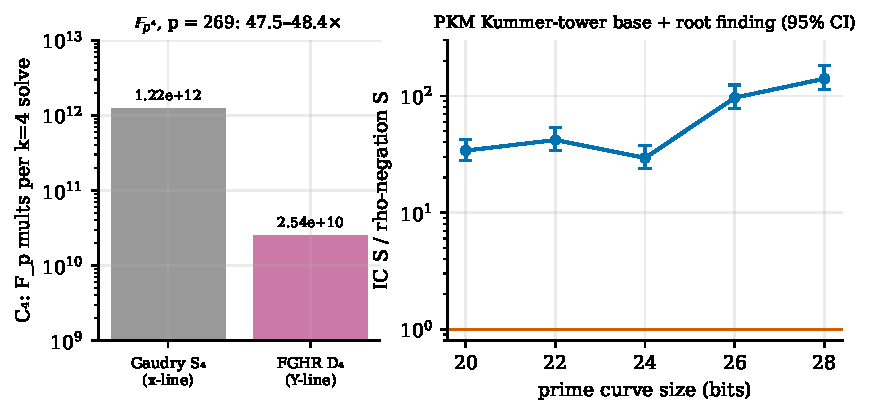
\includegraphics[width=\linewidth]{figures/fig-prime.pdf}
\caption[]{Left: cost $C_4$ of one $k=4$ decomposition over $\FF_{p^4}$,
$p=269$, Gaudry's $S_4$ system on the $x$-line against FGHR's $D_4$ system
on the $Y$-line (\art{research/gaudry_quartic_d4_20261013/}). Right:
index calculus with the PKM tower base and root finding over rho with
negation, eight one-target workloads $\times$ three rounds per size,
paired 95\% cluster-bootstrap intervals
(\art{research/pkm_tower_ecbench_20261013/}).}
\label{fig:prime}
\end{figure}

\chapter{Extension fields: $k=4$ and the $D_4$ symmetry}\label{ch:extension}

Over $\FF_{q^k}$ with a factor base of points whose abscissa lies in
$\FF_q$, Gaudry's index calculus~\cite{gaudry2009} decomposes each target
into $k$ summands by Weil restriction of $\Sem{k+1}$. It costs
$\tilde O(q^{2-2/k})$, below rho's $q^{k/2}$ for $k\ge3$, but with a
Gröbner constant that grows very fast in $k$. Faugère, Gaudry, Huot and
Renault~\cite{fghr2014} show that on curves with rational 2-torsion the
system has the larger symmetry group $D_k$, the Weyl group of type D, in
a well-chosen coordinate. At $k=4$ this chapter reports how far that
symmetry moves the measured gap to rho. Chapter~\ref{sec:prime}
(\S\ref{sec:gaudry}) gives the odd-characteristic engineering in detail.

\section{The $D_4$ system}

On $E$ with rational 2-torsion point $T$, the coordinate
$Y=(x-x_0-c)/(x-x_0+c)$ satisfies $Y(P+T)=-Y(P)$. In $Y$, $\Sem5$ is
invariant under $D_4$, of order 192. Written in the invariants
$\sigma_k=e_k(Y_i^2)$ and $\pi=\prod Y_i$, the system shrinks:
\begin{itemize}
\item the Bézout number falls from 4{,}096 to 512;
\item the Macaulay degree falls from 29 to 14;
\item the matrix falls from $41{,}780\times40{,}920$ to $13{,}412\times11{,}628$.
\end{itemize}
The engineering ladder, each step against the previous incumbent, was:
\begin{enumerate}
\item \emph{$D_4$ invariants.} One decomposition costs $C_4=2.54\cdot10^{10}$
  $\FF_p$ multiplications instead of $1.21\cdot10^{12}$ at $p=269$, a
  factor of $47.5$--$48.4$. All 19 solved targets agree with an independent
  meet-in-the-middle enumeration
  (\art{research/gaudry_quartic_d4_20261013/}).
\item \emph{The $Y$-line on a complete ladder.} On $p=101$--$1033$ (21
  curves) the cost is $0.0548$ $[0.048,0.061]$ of plain $\Sem4$, at the same
  exponent.
\item \emph{Sparsest pivots, the weighted grading $\sigma_4=\pi^2$, and shape
  replay.} $C_4$ falls to $6.89\cdot10^7$, by $369.8\times$
  $[367.9,371.6]$; all 648 of 648 solves are exact. Ecbench $S$ falls
  $398$--$406\times$ (\art{research/gaudry_quartic_d4_cost_20261014/}).
\item \emph{First-dependency stop.} The cost is $0.979$ $[0.973,0.986]$ of the
  previous step. Double large primes cut the linear algebra to $0.827\times$
  but regress the whole solve, to $1.025\times$.
\item \emph{A Frobenius-reduced form in characteristic two.} Weights
  $(2,2,1,1)$ give Macaulay degree 11 and a $384\times448$ matrix. One
  decomposition is $481\times$ $[479,483]$ below the plain form at $m=8$
  (\art{research/gaudry_quartic_d4_char2_20261015/}).
\end{enumerate}
The $D_n$ symmetry is FGHR's~\cite{fghr2014}. Invariant rings in
characteristic two, including even-power substitutions, were studied by
Galbraith and Gebregiyorgis~\cite{galbraith2014}. Whether the
Frobenius-reduced weighting is in that work has not been checked.

\section{Distance to rho}

\paragraph{Odd characteristic.} Over $\FF_{p^4}$, index calculus is still
$1.39\cdot10^6\times$ rho at the measured sizes. The modelled handover
moves from $2^{150}$ to about $2^{103}$--$2^{119}$, depending on the frame,
but that is an extrapolation through a measured constant.

\paragraph{Characteristic two.} Over $\FF_{(2^m)^4}$ the gap closes with
size. IC over the negation-map rho model is:

\smallskip
\begin{tabular}{@{}lrrrrr@{}}
\toprule
$m$ & 6 & 8 & 10 & 12 & 14 \\
$\log_2 n$ & 24 & 32 & 40 & 48 & 56 \\
\midrule
IC / rho model & 5{,}080 & 648 & 80.6 & 49.7 & 6.06 \\
IC / measured rho & 4{,}427 & 919 & 98.9 & 47.2 & 4.27 \\
\bottomrule
\end{tabular}
\smallskip

\noindent These are first targets; $m=14$ is a single target. The fitted
slope is $-0.248$ in $\log_2 n$, which is Gaudry's $n^{-1/4}$. The
extrapolated crossover was $n\approx2^{68}$, where rho takes about $2^{34}$
steps, so it could be tested directly.

\paragraph{The red-team verdict.} An adversarial review tested that
crossover (\art{research/gaudry_k4_char2_redteam_20261026/REPORT.md}). Its
verdict: \textbf{not survived (unsupported), not refuted}.
\begin{itemize}
\item \emph{Data.} The only clean point is at $m=15$, with two targets per
  arm. The recorded IC/rho there is $6.30$. After the corrections that
  favour index calculus it is $5.2$, with range $2.4$--$15.0$ over
  unit-price variants. The $m=17$ ratio of $0.72$ came from a killed run
  and is not evidence. No interval is possible with $n=2$.
\item \emph{Rho reference survives.} These are generic ordinary curves with
  $\operatorname{Aut}=\{\pm1\}$, and the floor $0.886$ is about 3.5\%
  generous to rho.
\item \emph{Pricing partly survives.} The unit price moves the ratio by
  $0.64$--$0.89$, with a plausible range of $0.31$--$3.1$. Unpriced rho
  work moves it by about $0.93$.
\item \emph{Fitted exponents} (cost in $q=2^m$): IC relations $1.07$
  $[1.01,1.13]$, IC linear algebra $2.03$, rho $2.00$ $[1.71,2.29]$. A
  prime-field cross-check agrees.
\item \emph{Corrected crossover.} The IC/rho ratio falls by about
  $2^{-0.93}$ per unit of $m$, which puts the crossover at
  $m^*\approx17.6$, with range $16.3$--$19.2$: at or above the edge of what
  was measured.
\end{itemize}
Linear algebra is 0.4\% of the cost at $m=15$. Basic Gaudry linear
algebra grows as $q^2$, like rho, so the $n^{-1/4}$ trend lasts only while
the relation phase dominates. Beyond that point double large primes are
required.

The red team froze a plan to settle the question: $m=14$--$17$, eight fresh
targets per arm, a strong rho with batched inversion and charged
canonicalisation, counted and hardware units, about 30\,h of wall time.
It has not run. This is the cheapest experiment in the programme that
could yield a measured crossover of index calculus below rho on an
elliptic curve. It would be a crossover in a weak family:
$\FF_{(2^m)^4}$ is not a field deployed curves use.

\section{Other extension-field routes}

\begin{itemize}
\item \emph{Joux--Vitse $(n-1)$-decomposition.} The
  $(n-1)$-decomposition~\cite{jouxvitse2012} at $n=5$ over $E(\FF_{p^5})$
  completed verified logarithms at $4.5\cdot10^7$--$1.8\cdot10^8\times$ rho,
  with a crossover extrapolated to groups near $2^{291}$
  (\art{research/joux_vitse_n1_20261015/}).
\item \emph{Joux--Vitse cover.} The cover of $E(\FF_{p^6})$ is in
  Chapter~\ref{sec:transfer}.
\end{itemize}

\chapter{Covers, isogenies and other transfers}\label{sec:transfer}

A recurring hope was that some other representation of the same
instance---an isogenous curve, a curve at another level of the isogeny
volcano, a Jacobian, a Weil descent---would make index calculus cheaper.
These routes produced the programme's clearest negatives, and one lemma
that explains most of them.

\begin{lemma}[transport conservation,
\art{docs/ic/RESEARCH_TRANSFER_AWARE_IC_20261010.md} \S1]\label{lem:conservation}
Let $\varphi:E\to E'$ be an $\FF_q$-rational isogeny (or any homomorphism
of rational points), $\kappa=\ker\varphi\cap E(\FF_q)$, $R\in E(\FF_q)$,
$\Fb'\subset\varphi(E(\FF_q))$ a factor base on the codomain and
$\Fb=\varphi^{-1}(\Fb')\cap E(\FF_q)$. Then the number of ordered
$m$-decompositions of $R$ over $\Fb$ is $\abs\kappa^{m-1}$ times the number
of ordered $m$-decompositions of $\varphi(R)$ over $\Fb'$.
\end{lemma}
\begin{proof}
Images of decompositions of $R$ are decompositions of $\varphi(R)$.
Conversely, for $\sum Q_i=\varphi(R)$ choose rational preimages $P_i$ of
the $Q_i$; then $\sum P_i-R\in\kappa$, and of the $\abs\kappa^m$ choices
exactly $\abs\kappa^{m-1}$ sum to $R$ (translate $P_1$ by the kernel
element).
\end{proof}

So a homomorphic transfer changes nothing but three curve-specific inputs:
the rational kernel symmetry $\abs\kappa^{m-1}$ (bounded by the rational
torsion; trivial on prime-order curves), the factor-base geometry
available on the destination, and the cost of arithmetic there. Sequences
of isogenies compose to one homomorphism; a loop is an endomorphism and
acts on the subgroup as a known scalar, useful only as a known-log
multiplier. Multi-curve factor bases glued by isogenies are single-curve
bases in disguise.

\paragraph{Conductor gaps in the ECC2K-130 class.} Jao, Miller and
Venkatesan~\cite{jmv2005} prove random self-reducibility among curves with
the same endomorphism ring, leaving open whether curves whose conductors
differ by a large prime could differ in hardness. The ECC2K-130 class has
conductor gap 263; we computed its structure
(\art{docs/ic/RESEARCH_ISOGENY_CONDUCTOR_GAP_20261007.md}) and ran
several rounds of experiments. Native counted-$S$ index calculus on two fixed CM
pairs gave floor/crater ratios $0.975$ (99\% $[0.603,1.451]$) at
$\ell=8209$ and $1.127$ $[0.922,1.342]$ at $\ell=131101$: no level effect
(192 verified records, 96 exact replays;
\art{research/ecbench_conductor_gap_20261012/}). Two-torsion
symmetrisation is a quotient isogeny: at a matched base of abscissae it
cut F4 row-reduction work $4.1$--$4.3\times$ ($\abs H=2$) and
$17.6$--$19.6\times$ ($\abs H=4$) over 1{,}128 systems---but a correction
the next day showed that at a matched number of \emph{columns} the saving
disappears; it was the cost of a redundant orbit base. A combined Weil
descent used $234$--$529\times$ the F4 operations of the blind system
(\art{research/isogeny_conductor_gap_round3_20261011/}).

\paragraph{Fibre-aware index calculus.} Isogeny fibres are torsors whose
arithmetic is controlled by one cohomology class
(\art{RESEARCH_ISOGENY_FIBERS_ECDLP.md}); relation generation is
isogeny-equivariant at zero lifting cost, and a fibre-closed pair table was
the best lever of the conductor-gap rounds ($12.8\times$ rho in its best
cell). Measured against matched rho across sizes at fixed cofactor, the
envelope IC/rho ratio grows from $8.4$--$8.8$ to $35.1$--$37.0$ ($h=4$) and
from $13.4$--$20.1$ to $60.4$--$63.1$ ($h=72$), as $\#E^{1/6}$: the gap
widens, it does not close (816 audited records;
\art{research/fiber_ic_scaling_20261011/}).

\paragraph{Other structure.} Symmetrised $u$-frame bases saved
$0.84\times$ at $n=17$ and $0.76$--$0.77\times$ at $n=23$, but cost
$4.01\times$ at $n=31$ (\art{research/koblitz_symmetrised_e2e_20260927/}).
GHS and hyperelliptic covers: ECC2K-130 does map to hyperelliptic curves,
but the genus that would pay is missing. In odd characteristic the cubic
GHS transfer from $E_0(\FF_{q^3})$ to a genus-3 Jacobian now runs end to end
with double-large-prime index calculus, at about $q^{1.4}$ against rho's
$q^{3/2}$, within $1.15\times$ of a measured negation-map rho at
$q=2^{20}$ (\S\ref{sec:ladder}). The
isogeny-loop GLV/GLS work produced a measured $1.09$--$1.15\times$ faster
four-dimensional scalar multiplication (\art{research/isogeny_loop_glv_20261012/})
and a $\sqrt{\text{\'elu}}$ kernel cost exponent $0.822$ $[0.805,0.838]$;
these speed up curve arithmetic, not the discrete logarithm.

\paragraph{Covers, 21--24 October.} The Joux--Vitse genus-3 cover of
$E(\FF_{p^6})$ is now within $1.6$--$2.0\times$ of a pooled rho constant at
$p=1009$; measuring the per-trial cost on a genus-255 binary Jacobian
turned the $N=130$ GHS counterfactual's modelled margin negative ($-1.83$
bits); and two censuses bound what covers exist at toy sizes (genus floor 13
for odd-order $E/\FF_{q^4}$; a $2^{-l}$ genus-3 fraction over
$\FF_{2^{3l}}$). All are in \S\ref{sec:ladder3}. None touches a prime field
or a prime-degree binary field, where the GHS genus is out of reach.

\paragraph{The published scale of high-genus index calculus.} The largest
Weil-descent hyperelliptic discrete logarithms in the literature are at
genus 31. Jacobson, Menezes and Stein~\cite{jms2001} applied GHS to elliptic
curves over $\FF_{2^{62}}$, $\FF_{2^{93}}$, $\FF_{2^{124}}$ and
$\FF_{2^{155}}$ and obtained genus-31 curves $C_{62}$, $C_{93}$, $C_{124}$
and $C_{155}$ over $\FF_{2^2}$ to $\FF_{2^5}$, each with $\#J=2r$, $r$
prime. They solved $C_{62}$, $C_{93}$ and $C_{124}$ with Enge--Gaudry
(relation collection for $C_{124}$ took 379 CPU-days on a mixed cluster) and
only estimated $C_{155}$, at 26{,}290 days on one 1\,GHz Pentium III.
Velichka~\cite{velichka2008} solved $C_{155}$ ($\#J\approx2^{155}$) with
Vollmer's algorithm and sieving: 136{,}533 relations, about 1{,}735 CPU-days
in total, 21 days wall-clock, of which 14 days were linear algebra. No genus
above 31 appears in that thesis; the journal version~\cite{vjs2014} was not
available to us and is unchecked. Our genus-255 per-trial measurement
(\S\ref{sec:ladder3}) is a cost sample, not a solved instance, at about
eight times the largest published genus. The cover ECC2K-130 would need, of
genus about $2^{130}$ (\S\ref{sec:ecc2k130}), lies about $2^{125}$ times
beyond it.

\paragraph{Genus three against the strongest rho.} Rounds three and four
of the genus-3 work ran without a rho arm; a 23 October study supplied one
(\art{research/ghs3_vs_rho_20261023/}; it has a frozen protocol and tables
but no README, and no review is recorded in it). On round 4's instances,
$q=2^{14}$ to $2^{20}$, three curves per size, in round 4's unit and binary,
the reference was an ideal negation rho priced with Karatsuba products and
32 walks per inversion ($R_{\mathrm{ideal}}$, the primary reference, the
most favourable to rho) and a measured negation walk ($R_{\mathrm{meas}}$).
The frozen rule declares ``IC below the strong rho'' at a size only if every
curve is below both references at every weight of the band. At $q=2^{16}$
it is: IC/$R_{\mathrm{ideal}}$ is $0.70$, $0.71$, $0.70$ at $w=0$ and $0.64$
and $0.38$ (geometric means) at $w=0.1$ and $1$. At the other six sizes the
decision is \emph{unresolved}, with geometric means $0.97$--$1.52$ ($1.27$ at
$2^{20}$). Three things qualify the result. The registered unit prices one
subgroup multiplication as one $\FF_q$ multiplication ($c_\ell=1$); the
protocol's own sensitivity, $c_\ell=9$, puts every instance at $2.7$--$12.4\times$
rho. The ratio carries $\sqrt c$ of the cofactor, because IC depends on $q$
alone and rho on $\ell=\#E_0/c$: the three curves at $2^{16}$ all have
cofactor 4, and a post-hoc fit gives exponent $0.474$ in $c$ (theory $0.5$)
and $-0.081$ per bit of $q$ at fixed $c$ (theory $-0.167$). And the pooled
trend over all 21 instances is flat ($0.034$ $[-0.047,0.105]$ per bit), so
no crossover size is determined. This is the programme's only
preregistered decision of index calculus below the strongest rho. It is a
measurement of a known pipeline in a structured, weak class
($E_0/\FF_{q^3}$ with $4\mid\#E_0$, never prime order), where theory
predicts $q^{4/3}$ against $q^{3/2}$; it depends on the pricing of one
operation; and it is not yet reviewed. It updates the ledger paper's
``$1.15\times$ at $2^{20}$'' and bears on that paper's prediction of a
crossover at $q\le2^{22}$ once rho is measured: below rho at one size,
unresolved at the others, with no measurable pooled trend.

\paragraph{The same family through a plane quartic.} The $m=2$ type of the
cubic GHS cover gives a smooth plane quartic over $\FF_q$ directly. On a
plane quartic, Diem's index calculus is $\tilde O(q)$ in theory, against
$q^{4/3}$ for the hyperelliptic genus-3 route above. Before 18 October the
repository's plane-quartic ``pure IC'' toys could not be priced: their
logarithms came from enumerating the subgroup, and the degree-3 class keys
merged distinct classes. A canonical $\mathrm{Pic}^0$ arithmetic now gives
every class a unique key (checked against brute-force class counts on 21
curves and full Cayley tables at $q=5$). A generic addition costs 3{,}523
multiplications and 44 inversions, flat in $q$ up to $2^{31}-1$
(\art{research/quartic_pic_canonical_20261018/}).

On that arithmetic, a pipeline with relations on lines, a reduced factor base
with one large prime, Lanczos modulo $\ell$ and canonical descent solved and
verified 51 of 51 units. It ran on the GHS-weak family $E_0/\FF_{q^3}$ with
$4\mid\#E_0$, for $q=223$ to $262{,}111$ (\art{research/quartic_n4_20261019/}).
\begin{itemize}
  \item Its reference is a matched \emph{plain} rho, without the negation
    map, on the same subgroup.
  \item At $q=262{,}111$, index calculus costs $0.122$ $[0.10,0.16]$ of that
    rho in $\FF_q$-multiplication equivalents. The order holds across the
    pricing band for every $q\ge4051$.
  \item The fitted exponents on $q\ge4051$ are $1.083$ $[1.040,1.129]$ for
    index calculus and $1.485$ $[1.437,1.525]$ for rho.
  \item In wall time, index calculus is cheaper only above $q\approx3\times10^4$.
\end{itemize}
This was a preregistered decision of index calculus below a matched
\emph{plain} rho. Its successor, N4~v2
(\art{research/quartic_n4v2_20261020/}, 20--25 October), took the same
family and instances from $q=2^8$ to $2^{22}$ (63 instances, 501 index-calculus
units and 2{,}442 rho runs, all verified) and added three changes: double
large primes (D), structured Gaussian elimination with Lanczos (L), and a
negation-map rho. Against the frozen pipeline B0 at $q=2{,}097{,}091$:
\begin{itemize}
  \item D costs $0.081$ of B0 and the combined arm DL $0.042$ $[0.042,0.042]$;
    a post-hoc arm DL1 reaches $0.022$.
  \item DL's fitted exponent is $0.983$ $[0.975,0.993]$ over the full range
    and $0.988$ on $k=17..22$, which is the $\tilde O(q)$ of Diem's
    analysis~\cite{diem2006,dt2008}; negation rho fits $1.543$ $[1.494,1.583]$.
  \item DL over negation rho is $0.005$ $[0.004,0.008]$ at the top size,
    with an interpolated crossover at $q^*=555$ $[389,752]$ in counted
    units ($q^*\approx1{,}889$ in CPU time). At $q=4{,}194{,}271$ one solve
    took $12.3$ CPU-seconds against 616 for negation rho.
\end{itemize}
The qualifications are substantial. The host was L0 (load average 22--60);
the intervals resample only three units per size at $k\ge17$; the
conversion constants move D's high-range exponent from $1.009$ to $1.048$;
the frozen B0 records do not replay at any of 11 replayed sizes; the
negation rho fails the calibration rule at three sizes; and there is no
validation file. The program's closing note calls the result ``our
measurements of a known result''
(\art{research/plane_quartic_program_20261018/CLOSING.md}). It covers the
GHS-weak family only; nothing here is about a generic curve, a prime-order
curve or a standard curve.

\paragraph{Smith's isogeny and the walk to it.} The other genus-3 type of the
census is hyperelliptic. Smith's $(2,2,2)$-isogeny takes it to a plane quartic
when his Propositions~2 and~4 pass. The walk study looked for curves on which
Smith's construction succeeds by walking 2-isogenies on the elliptic side
(\art{research/smith_elliptic_walk_20261018/}).
\begin{itemize}
  \item Exhaustively at $p=7$ to $31$, $0.53$--$0.61$ of the descended curves
    pass Smith's full test, against $0.1857$ for random curves. The
    preregistered expectation of about $0.186$ is falsified, upward.
  \item A failing curve has a passing one in its 2-isogeny component in
    $0.74$--$0.98$ of cases, at a mean distance of $1.5$--$3.6$ steps.
  \item On sampled walks at $p=2^{10}$ to $2^{20}$, the frozen fit labels the
    walk cost $o(p)$, with exponent $-0.14$ $[-0.80,0.95]$.
  \item A labelled post hoc analysis attributes that label to censored walks
    at the small primes. Successful walks at $p\equiv3\pmod4$ scale as
    $p^{1.13}$ $[1.00,1.26]$ in cost, which reads as $\tilde\Theta(p)$.
  \item At $p\equiv1\pmod4$ most walks stay inside small trapped sets.
\end{itemize}
A second study, also open and not yet merged, maps divisor classes through
Smith's isogeny and runs the whole route at toy sizes. The program's closing
note lists what stays open (\art{research/plane_quartic_program_20261018/CLOSING.md}).

\paragraph{Joux--Vitse: two arms of one cover.} The Joux--Vitse cover of
$E(\FF_{p^6})$ (full rational 2-torsion, a weak class) has been measured
with two solvers, and their comparisons with rho do not agree. The
\emph{plain Nagao arm} with a sparse-FGLM linear stage is $1.59$--$1.98\times$
a pooled rho constant at $p=1009$ and closes as about $p^{-2}$
(\art{research/jv_cover_p_scaling_20261024/}; \S\ref{sec:ladder3}); it is a
lower-bound comparison and current. The \emph{sieve arm}
(\texttt{jv\_cover --exp sieve}) measured $0.024$ $[0.019,0.031]$ of a strong
rho at $p=1009$ and $0.0042$ at $p=1823$ on 19 October, but its 20 October
review withheld every comparison (no numeric acceptance for the controls,
uncharged rho hashes, incomplete accounting;
\art{research/jv_sieve_strong_rho_20261019/}); a replication with fixed
thresholds failed its acceptance rule and is in an open pull request, and a
prospective re-run is registered and has not run. A 9 October whole-route
replay from a non-weak challenge curve, through an isogeny walk to a weak
curve and its cover, read $0.058$ of a pooled, unmatched rho at $p=1009$ on
one seed per prime, with an earlier revision of the solver whose source
includes the sieve module (\art{research/jv_cover_e2e_30bit_20261009/RESULT.md}).
The roughly thirtyfold gap between the arms at $p=1009$ is unexplained on
\texttt{main}. The cover-decomposition note still states a measured sieve
crossover near $p\approx430$
(\art{research/notes/index-calculus/RESEARCH_COVER_DECOMPOSITION_LEDGER.md}
\S11) with no erratum; it should be read through the review. Leaderboard
Table~D, the historical study, is withheld. On the method side, the
sparse-FGLM stage made the plain arm $1.28\times$ cheaper end to end
(\art{research/jv_cover_sparse_fglm_20261018/}); relation collection is
$99.99\%$ of $S$ (\art{research/ic_cover_leads_20261018/}); depth-1 isogeny
classes hold no weak curve over 4{,}871{,}062 curves, while 86--95\% of
deeper classes hold one (\art{research/jv_weak_class_law_20261007/}); and
the $(n-1)$-decomposition variant is $4.5\cdot10^7$--$1.8\cdot10^8\times$
rho (\art{research/joux_vitse_n1_20261015/}).

\paragraph{Cover censuses.} The minimal cubic GHS genus over an isogeny
class follows $\#E(K)\bmod4$: 13 for odd order, 5 for $2\bmod4$, 3 for
$0\bmod4$, and genus 3 is the only value below rho's $q^{3/2}$
(\art{research/ghs_cubic_cover_census_20261012/}); at $n=5$ the floors are
33, 33, 25 and 5 by 2-torsion type (\art{research/ghs_cover_census_n5_20261013/}).
No deployed prime-field or prime-degree binary curve has a usable subfield;
only the RFC~2409 Oakley groups 3 and 4 are reachable, at genus 15--16, where
exponent models disagree in sign and the measured genus-16 relation phase
alone is 5.2 bits slower than rho (\art{research/cover_route_prime_binary_20261008/},
\art{research/ghs_oakley_extended_20261023/}). All 15{,}791 cover maps in the
registry were assessed: 165 binary maps have genus-3 arithmetic and the
15{,}626 odd-characteristic genus-2 covers lack a Jacobian implementation
(\art{research/cover_transfer_assessment_20261013/}). An inventory of about
90 cover and decomposition studies found every route on prime, Koblitz and
prime-degree binary curves closed, negative or constant-factor
(\art{research/cover_decomposition_gap_search_20261018/}). Smith's
$(2,2,2)$-isogeny route was reproduced natively (full success $0.18638$
against a theoretical $0.18574$ over $10^6$ curves) and its sign bias shrinks
like $1/\sqrt p$ (\art{research/smith_prop24_native_20261014/},
\art{research/smith_sign_scaling_20261016/}).

\paragraph{Volcano levels and generators.} A 403{,}168-run census found the
level effect equivalent in 33 of 35 comparisons and different in none
(\art{research/volcano_ecdlp_census_20261017/}), and a large-sample rho study
found the floor/crater ratio $0.998$ $[0.986,1.010]$
(\art{research/conductor_gap_rho_large_sample_20261018/}). The one real level
effect is the automorphism group: $\sqrt3$ on the $j=0$ crater, confirmed at
$1.86$--$1.92\times$ (\art{research/drastic_prime_conductor_gap_round3_20261012/}).
At $\ell=2$, floors give $5.8\%$ fewer relations than craters, and 99\% of the
contrast is explained by the base's cofactor classes
(\art{research/isogeny-volcano-cost-v2_20261017/},
\art{research/generator_effect_ic_20261019/}).

\paragraph{Other transfer lines.} Index calculus on genus-2 to -4
Jacobians over $\FF_p$ (the ADH--Gaudry attack, measured against rho on the
same Jacobian) read below a distinguished-point rho in early rounds, but the
reference was later found slow and the ratios are lower bounds, unranked
under the band (\art{research/notes/index-calculus/RESEARCH_HYPERELLIPTIC_IC_RHO.md});
later rounds are in review. A weak-curve atlas of 922 exact models and 36
published cases ranks covering-model and pairing signals but leaves the
selected-subgroup advantage unmeasured
(\art{research/weak_curve_leaderboard_20261012/}); three complete isogeny
volcano graphs (24{,}823 vertices) were built and their graph-wide IC
surveys halted at checkpoints (\art{research/full_volcano_graphwide_ic_20261017/}).
Weil restriction of ECC2K-130 to extension fields costs at least $2^{131}$,
$2^{70.19}$ times rho (cluster ``transfer-boundaries'').

\paragraph{Named obstructions.} Blocked requirements are kept open as
problem records (\art{problems/README.md}), among them the complete-cost
calibration of root-finding IC
(\art{problems/rootfinding-complete-cost-calibration.md}), with exit
criteria rather than abandoned.


\part{The frontier}\label{part:frontier}
\chapter{The summer record: July--September 2026}\label{ch:summer}

The October campaign measured in the rest of this part did not begin from
nothing. Between 19 July and 30 September the crypto-autoresearcher ledger
recorded 1{,}402 coordinator decisions on ECDLP and index calculus:
\begin{itemize}
\item July: 74 decisions on 20 experiments, 977 run directories;
\item August: 364 decisions on 92 experiments, 321 run directories;
\item September: 964 decisions on 449 experiments, 776 run directories.
\end{itemize}
Each decision names a verdict, the hypotheses and experiments it rules on,
and the evidence it cites. The dated index
(\art{research/ecdlp_jul_sep_index_20261029/}: \texttt{INDEX.json},
\texttt{INDEX.tsv}, and the generator \texttt{build\_index.py}) lays these
out together with the run-data path of each experiment. A decision is
counted as ECDLP work if its goal is one of 19 ECDLP goals or, when it names
no goal, if a target or evidence identifier carries an ECDLP family token.
That scope rule is a choice and is stated in the generator. Seven decisions
filed under late-September names carry October dates and are left out
of the counts above. Twenty-three decision files did not parse and are not
indexed.

\begin{figure}[t]
\centering
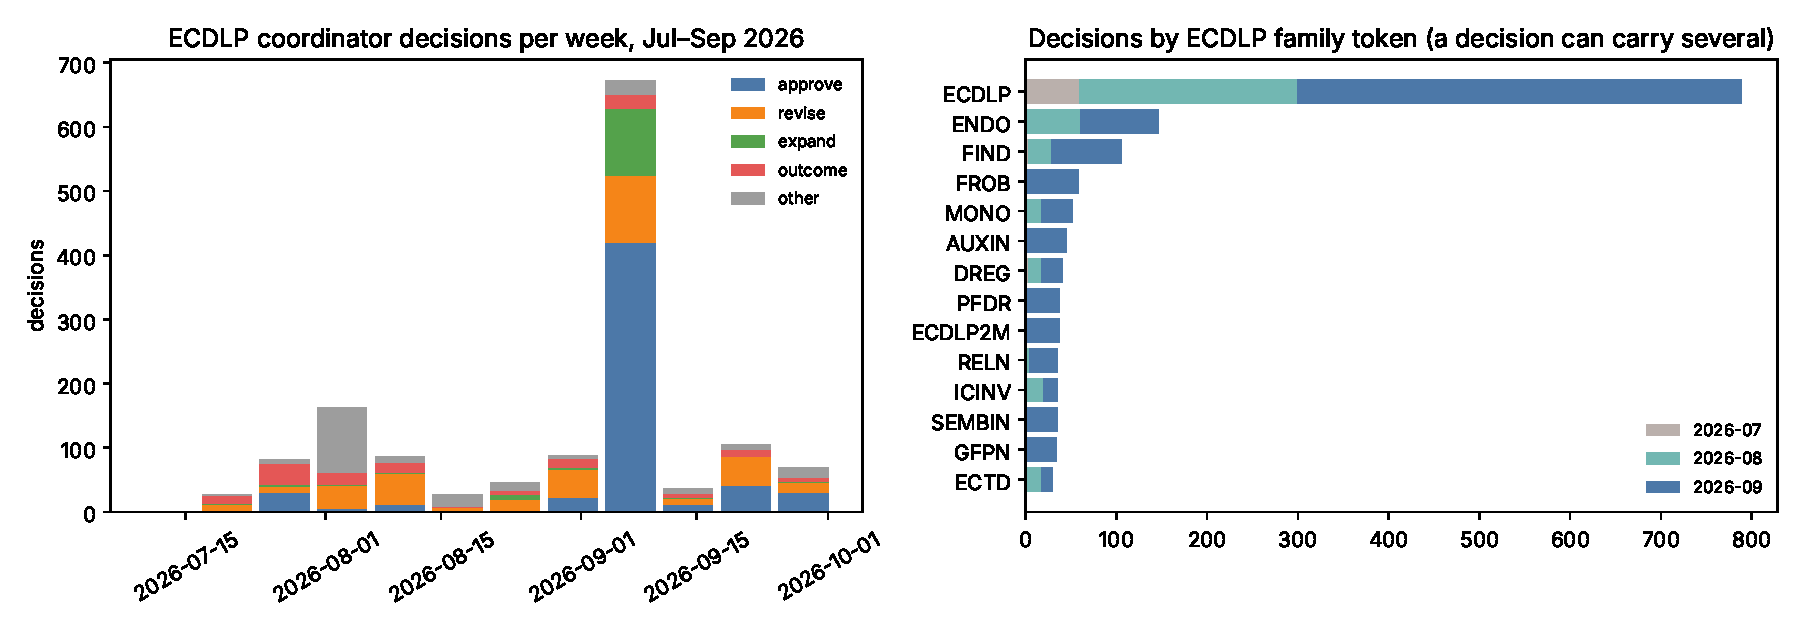
\includegraphics[width=\textwidth]{figures/fig-jul-sep.pdf}
\caption{ECDLP coordinator decisions, July--September 2026. Left: decisions
per week by verdict class. The class \emph{outcome} groups support,
reject\_scoped, weaken, inconclusive, supersede and pause. Right: decisions
per family token, by month; a decision can carry several tokens. The week
of 7 September holds 672 decisions, most of them approvals of frozen stage-0
contracts.}\label{fig:julsep}
\end{figure}

Most of this activity was process (Figure~\ref{fig:julsep}). Of the
1{,}402 decisions, 561 approve a contract, 267 revise one and 124 expand
one. About 157 carry an outcome on a hypothesis (support, reject, weaken,
inconclusive, supersede, pause or replicate). This chapter reports
those outcomes by theme, with decision identifiers so that each can be
traced. All results are at toy or derivation tier unless a scale is given.
None moved an exponent on a prime field.

\section{July: the first baseline and two retracted wins}

The ledger's first ECDLP decision, \texttt{DEC-20260719-001}, expanded a
toy Semaev $S_3$ Gröbner study (\texttt{EV-SEMAEV-001}). It had twelve runs
at 8--12 bits with a factor base of 14 points. The degree proxy stayed at
most 4 and the wall time stayed flat near 0.16\,s. The decision itself
noted that three bit sizes and two seeds cannot establish a trend.

Two supports followed on 26 July, and both were overturned the next day:
\begin{itemize}
\item \emph{Index calculus beats enumeration} (\texttt{H-IC-001}, 748 runs
  at 8--36 bits) was weakened by \texttt{DEC-20260727-008}. The criterion
  had been revised after the outcome. There were no decompositions at 20
  bits or above, so the measured descent time was the cost of a failed
  attempt. The relation cost was $2287\times$ the group order at 36 bits.
  The decision records: ``no asymptotic exponent moves''.
\item \emph{A structured factor base induces sparsity} (\texttt{H-STR-002})
  was weakened by \texttt{DEC-20260727-009}. Three headline instances had
  no run records. The one-variable ablation gave $\alpha=27,52,197,386$
  against $27,52,199,387$ for a random base, so the factor base induced
  nothing.
\end{itemize}
In the same week a generic-group classifier (\texttt{EXP-GGM-001}) had its
support revoked (\texttt{DEC-20260727-007}). It was a lookup table, and its
nine runs were byte-identical. Fixed-curve preprocessing showed no robust
gain over 72 runs (\texttt{DEC-20260726-001}, paused). A subresultant
degree exponent was measured at $\beta_{\rm deg}=0.5985$ against a gate of
$0.3$ (\texttt{DEC-20260728-003}, weakened).

Xedni-style lifting was closed in exact form (\texttt{DEC-20260724-021},
reject\_scoped): $P_{\rm lift}=(1-2/p+p^{-3})/(2p^3)$, so $\alpha=3$. This
is the result restated in Chapter~\ref{ch:obstructions}.

\section{August: yield, monodromy, oracles and transfers}

\paragraph{Yield matches the heuristic from below.} Semaev decomposition
yield at $m=2$ reached $0.80$, $0.98$ and $1.00$ of the $B^m/(m!N)$
heuristic at $p=1009$, $4001$ and $9001$ (\texttt{EV-YIELD-e1adbf}).
\texttt{DEC-20260804-9da614} weakened super-heuristic yield at $m=2$--$4$.
Structured bases gave small-$x$ $0.845$, arithmetic progression $0.658$
and random $0.563$, with no super-heuristic yield
(\texttt{DEC-20260804-2bfc30}). These measurements came before the
conservation proposition of Chapter~\ref{ch:cover}, which explains them: at
matched base size the mean is fixed. A complete $m=2$ index calculus solved
a discrete logarithm at $p=1009$ (\texttt{DEC-20260804-db75bb}). A
Fourier-flatness constant for the factor base was fitted as
$C(p)\sim p^{0.055}$--$p^{0.079}$ and recorded as an open problem
(\texttt{H-PSEUDO}). Eight proof routes were closed as non-proving.

\paragraph{BKK and meet in the middle: constant factors.} A BKK sparsity
argument promised a speedup of at least $(m+1)/2$
(\texttt{DEC-20260804-1825ea}). It measured $1.99988$ against $2.0$ at
$m=3$ on a smoke test. \texttt{DEC-20260806-26c0e8} then found the
multi-target window empty at the planned sizes and the gain about
$1.0$--$1.8\times$. Meet-in-the-middle structure gave $18\times$, which rho
dominates (\texttt{DEC-20260808-030b1f}). A degree-split claw lost its
advantage to a matched null, $R=0.0472$ against $0.0311$
(\texttt{DEC-20260801-005}). The decision reads: ``the instrument, not the
hypothesis, has been refuted''.

\paragraph{Monodromy.} The work that became Chapter~\ref{ch:cover} was
done in August:
\begin{itemize}
\item the $m=3$ derivation (\texttt{DEC-20260802-a51c82});
\item the all-$m$ theorem, supported as scoped and ``not closed''
  (\texttt{DEC-20260807-64df6a}, \texttt{KN-FIND-a8990a});
\item containment in $(\ZZ/2)^{m-2}$ at $m=4,5$ on eight curves, with zero
  exceptions in an exhaustive census of 2{,}915{,}514 triples at $p=103$
  (\texttt{DEC-20260830-0f8def});
\item monodromy $D_4$ for the $m=3$ symmetric-base cover
  (\texttt{DEC-20260830-1fb2e3}).
\end{itemize}
The fibre census was ruled blind to relation rate as an instrument
(\texttt{DEC-20260810-2f86db}, reject\_scoped), two months before the
census corollary proved why.

\paragraph{Oracles and transfers.} Two analysis-only results bounded the
oracle leads. Oracles C and D are simulable in the generic group model, and
A and B give no sub-birthday advantage (\texttt{DEC-20260804-3b4258},
support\_scoped). The doubling oracle was then shown equivalent to an
$x$-coordinate oracle (\texttt{DEC-20260806-08b9ed}). Three transfer and
invariant routes were closed:
\begin{itemize}
\item Isogeny transfer: the anomalous, MOV and Weil-descent families are
  invariants of the isogeny class (\texttt{DEC-20260804-2fae6a}).
\item Elkies augmentation: with $\ell\le23$ it matched a random-bijection
  null to within $0.004$ in all eight cells at 20--28 bits
  (\texttt{DEC-20260804-d0c452}).
\item CM: complex multiplication changes the lifted-height obstruction ``by
  exactly nothing'' (\texttt{DEC-20260810-2c7e3c}).
\end{itemize}
Within one isogeny class the over-dispersion of ECDLP-relevant statistics
traced to the 2-torsion type (\texttt{DEC-20260811-a3398a},
\texttt{KN-FIND-ddd982}).

\paragraph{Degree of regularity.} The boolean chained $m=3$ system was
run at $n=21$, $D=5$, and stopped at rank $265{,}950$ of a predicted
$268{,}674$ (\texttt{EV-DREG-4500cd}). The record calls this ``not evidence
about $d_{\rm reg}$ in either direction''. All six $n=15$ runs then
exceeded memory (\texttt{DEC-20260828-653923}). The certified
fall-degree results of Chapter~\ref{ch:falldegree} later replaced this
line.

Late August was spent on governance: budget ceilings, pauses and
zero-run successors. \texttt{DEC-20260820-0c8ffb} paused at the budget
ceiling. The ``fund every goal'' decisions of 28 August lifted the limits.

\section{September: tables, lifts, audits and the first binary costing}

\paragraph{Distinguished-point tables re-selected from the batch.} The
claim that a table of $T/2$ entries re-selected from solved walks matches a
static Bernstein--Lange table of $T$ was contradicted at $a=1/4$. It
reached $0.65$--$0.69\,T$ at steady state, with intervals excluding 1,
while paying $2.6$--$8.9\,T$ of working storage (\texttt{DEC-20260906-1f5b71},
weaken: ``a tradeoff point, not an improvement''). At $N=2^{24}$ the
feasibility crossing was then bracketed between $a=1/8$ and $a=3/16$
(\texttt{DEC-20260907-9b1b02}, \texttt{DEC-20260907-6d9427}). The result is
a ceiling only, with no online arm (\texttt{DEC-20260910-34e654}).

\paragraph{The canonical lift carries no logarithm.} The $p$-adic lift
statistic $D_1$ took exactly the values $\{0,8\}$ on 1{,}035 pairs at
$p=1009$, and the same in a third independent implementation and on a
second instance. It tracked precision $r=4,8,12$ exactly
(\texttt{DEC-20260903-256c7c}). The digit identity held in $1360/1360$
cases, and the Teichmüller contrast showed no inflation: all three ratio
intervals contain 1 (\texttt{DEC-20260911-74c9dc},
\texttt{DEC-20260912-2a626b}). Both results were recorded as ``no attack''.

\paragraph{Natural statistics are not biased enough.} An $L^1$ Fourier
registry over 406 cells and primes $4099$--$16{,}777{,}259$ falsified two
of its four predictions (\texttt{DEC-20260921-4516a0}, weaken):
\begin{itemize}
\item interval statistics: $\lambda=0.0806\pm0.0020$, against a
  prediction of at most $0.05$;
\item cosets and quadratic residues: $0.50$, against a prediction near 0.
\end{itemize}

\paragraph{Semaev degree and the Semaev 2015 / Nagao audits.} The
successful-subset loophole in the Semaev degree law was closed:
$\beta_{\rm work}=0.797$ worst case over 36 cells and 1{,}152 queries
(\texttt{DEC-20260929-780751}, reject\_scoped, \texttt{EV-SDEG-4a1c3d}).
The audits of Semaev's 2015 paper and Nagao's programme
(Chapter~\ref{ch:falldegree}) recorded these verdicts:
\begin{itemize}
\item eq.~(11)'s $\lambda$ is right to 1\% at $t=2$, but $P=1-e^{-\lambda}$
  fails by 18--22\% in the low-degree window (\texttt{DEC-20260913-3b51c8});
\item the typed-image ratio is not $m!$ at any of seven cells
  (\texttt{DEC-20260913-2386b5});
\item trace-parity confinement explains the whole deficit at $t=2$
  (\texttt{DEC-20260913-92aa48});
\item Nagao's memory claim fails at $n=571$, and 81 of the 120 flagged
  cells were an artifact of an incoherent memory pairing
  (\texttt{DEC-20260914-537000});
\item a published measurement claim, P3, fails under the corrected XOR
  product: the Semaev median is 2 in all eight cells, with the null at
  least one above it (\texttt{DEC-20260929-e37785}, reject\_scoped).
\end{itemize}

\paragraph{Prime-field degree versus yield.} A closed form for the first
fall degree of a digit-map presentation,
$d_{\rm ff}=m2^{m-1}+\lfloor(s-2^{m-1})/2\rfloor+1$, survived 26{,}000
instances with zero deviations. Its companion fall-dimension clause was
refuted by a certificate at $p=13$ (\texttt{DEC-20260904-1e27a2}). The
generator degree is $m2^{m-1}$, not $2m$, and the ``cells below rho'' of a
cost table had zero rows at $D_0$, so they were rejected
(\texttt{DEC-20260904-d47cd2}).

\paragraph{Frobenius-stable factor bases.} The stable subspaces are
exactly the ideals of $\FF_q[T]/(T^n-1)$, and the orbit count is exact on
14 of 14 cells (\texttt{DEC-20260922-5796b8},
\texttt{EV-FROB-d336b0}). The orbit gain is $n$, a constant factor. At
$n=131$ there are only four stable subspaces, and the orbit trick
\emph{loses} $57.0$--$96.0$ bits for $m=2$--$5$; at $n=163$ it loses
$72.7$--$121.7$ bits. Whether WDSat is blind to basis choice was never
measured, because 19 stage-0 launches failed.

\paragraph{The first costing of descended systems against rho.} The ICPERF
lane priced the descended algebraic normal form against the whole rho
budget on standard binary curves (\texttt{DEC-20260922-925da8},
\texttt{EV-ICPERF-784b25}). Forming the system alone exceeds rho by
$+6.3$ bits at $n=233$ and by $+40.8$ bits at $n=131$ (ECC2K-130).
Below $n\approx300$ the obstacle is building the system, not solving it.
The excess turns negative at $n=409$ and $571$ for $m\ge4$, and $m=2$
loses at every degree. This is the first September result priced against
rho. It is a model with measured inputs, not a solve.

\paragraph{Lanes without a result.} Several September lanes produced
approvals and redesigns but no measured outcome:
\begin{itemize}
\item SAT on summation systems, trapdoor detection, invariant calibrators
  and endomorphism decomposition, mostly frozen stage-0 contracts
  approved on 13 September;
\item the auxiliary-input census, whose run was ruled invalid as evidence
  because its controls were inadmissible and its escalation was generic to
  256-bit primes (\texttt{DEC-20260923-ce06a6});
\item EcGFp5 symmetrisation, where no $m=5$ ideal degree was measured
  (\texttt{DEC-20260923-d86ff2}), although the audit found that the curve's
  self-reported 323 bits recomputes to 322;
\item characteristic-2 quasi-subfield work, which found zero violations of
  its bound in about $340{,}000$ candidates and produced the derivation
  $\beta>1/2$ for every completely splitting $L$ (\texttt{KN-FIND-617d78}).
\end{itemize}
The certified binary refutations of Chapter~\ref{ch:falldegree} begin here:
$W_4$ refutes 62/62 at $n=17$ and 400/400 at $n=19$
(\texttt{DEC-20260924-e61f3b}, \texttt{DEC-20260926-901ea1}).

\begin{table}[p]
\centering\small
\setlength{\tabcolsep}{4pt}
\begin{tabular}{@{}llllp{4.6cm}@{}}
\toprule
month & theme & decision & verdict & recorded result \\
\midrule
Jul & IC beats enumeration & \texttt{DEC-20260727-008} & weaken & relation cost $2287\times$ the group order at 36 bits \\
    & structured factor base & \texttt{DEC-20260727-009} & weaken & $\alpha=27,52,197,386$ vs.\ random $27,52,199,387$ \\
    & subresultant degree & \texttt{DEC-20260728-003} & weaken & $\beta_{\rm deg}=0.5985$ vs.\ gate $0.3$ \\
    & xedni lifting & \texttt{DEC-20260724-021} & reject\_scoped & $\alpha=3$ \\
\addlinespace
Aug & Semaev yield, $m=2$ & \texttt{DEC-20260804-9da614} & weaken & $0.80$, $0.98$, $1.00$ of heuristic at $p=1009,4001,9001$ \\
    & BKK speedup & \texttt{DEC-20260806-26c0e8} & supersede claim & $1.0$--$1.8\times$, not $(m+1)/2$ \\
    & degree-split claw & \texttt{DEC-20260801-005} & weaken & $R=0.0472$ (null) vs.\ $0.0311$ \\
    & monodromy, $m=4,5$ & \texttt{DEC-20260830-0f8def} & support & 0 exceptions in 2{,}915{,}514 triples at $p=103$ \\
    & Elkies augmentation & \texttt{DEC-20260804-d0c452} & reject\_scoped & within $0.004$ of null, 8 cells, 20--28 bits \\
    & boolean $d_{\rm reg}$, $n=21$ & \texttt{DEC-20260815-6b806c} & supersede & rank $265{,}950$ of $268{,}674$; not evidence \\
\addlinespace
Sep & re-selected DP table & \texttt{DEC-20260906-1f5b71} & weaken & $0.65$--$0.69\,T$ at $a=1/4$ \\
    & canonical lift $D_1$ & \texttt{DEC-20260903-256c7c} & support & values exactly $\{0,8\}$ on 1{,}035 pairs; no attack \\
    & natural-statistic bias & \texttt{DEC-20260921-4516a0} & weaken & $\lambda=0.0806\pm0.0020$ vs.\ $\le0.05$ \\
    & Semaev degree loophole & \texttt{DEC-20260929-780751} & reject\_scoped & $\beta_{\rm work}=0.797$, 36 cells \\
    & Frobenius-stable bases & \texttt{DEC-20260922-5796b8} & support & loss of $57.0$--$96.0$ bits at $n=131$ \\
    & ICPERF costing & \texttt{DEC-20260922-925da8} & support & $+6.3$ ($n=233$) to $+40.8$ ($n=131$) bits over rho \\
\bottomrule
\end{tabular}
\caption[]{The summer record at a glance: one outcome decision per theme,
July--September 2026, with the number it recorded. Every row is
discussed above. Verdicts are the ledger's, shortened: ``weaken'' includes
\texttt{weaken\_h\_yield}, and ``supersede claim'' replaced the earlier
BKK support. Index: \art{research/ecdlp_jul_sep_index_20261029/INDEX.json}.}
\label{tab:summer}
\end{table}

\section{What the summer established}

Table~\ref{tab:summer} collects one outcome per theme. Four patterns run
through the 1{,}402 decisions:
\begin{enumerate}
\item \emph{No measured improvement over rho survived review.} Every
  July and August support that claimed a gain was weakened or revoked
  within days. The surviving gains are constant factors at toy scale.
\item \emph{The theory of Chapter~\ref{ch:cover} was found by
  measurement first.} The yield ratios at or below 1, the census ruled
  blind, and the exhaustive monodromy checks all preceded the proofs that
  explain them.
\item \emph{Most closures were instrument repairs.} A large share of the
  weaken and reject decisions say that a control, a metric or a criterion
  was wrong, not the hypothesis. This is the origin of the matched-null and
  replay rules of Chapter~\ref{sec:method}.
\item \emph{The binary line reached a priced verdict only in late
  September.} The ICPERF costing and the $W_4$ certificates opened the
  fall-degree and Koblitz work that the October campaign measured.
\end{enumerate}
These four patterns are the author's reading. The decisions cited above
are the record.

\chapter{What improved, and where the frontier stands}\label{sec:frontier}

\section{The measured frontier: one campaign, every cost priced}\label{sec:campaign}

The frontier synthesis of 13 October assembled ratios from studies that
used different curves, sizes and accounting. To replace it we ran one
campaign (\art{research/ic_frontier_campaign_20261015/}, protocol frozen
before any measured run). Every method family ran on the same fixed curve
ladders: eight Koblitz curves chosen by subgroup size
($\log_2 r\approx11$--$39$, $n\in\{13,17,19,23,37,41,43,47\}$), six
NIST-shaped $a=-3$ prime-order curves of 20--40 bits, and the five
2-adic curves of the Kummer-tower ladder. Each curve had 16 public
hash-to-subgroup targets nobody knows the logarithm of, 2 measured rounds
and a warm-up, and every answer was checked outside the solver. That is
4{,}848 executions, 3{,}232 of them measured: 3{,}178 verified and 54
exhausted, all of the latter in the shared-rank arm at $n=41$ and $n=47$.
Every session is audited by re-executing every measured run and
requiring identical counts. Index-calculus parameters (compact-orbit
columns, negfold subspace dimension, prime base size) were chosen per size
on a disjoint set of training targets, with grids widened until the
optimum was interior. Every cost is reported across the pricing band of
\S\ref{sec:band}.

\begin{figure}[t]
\centering
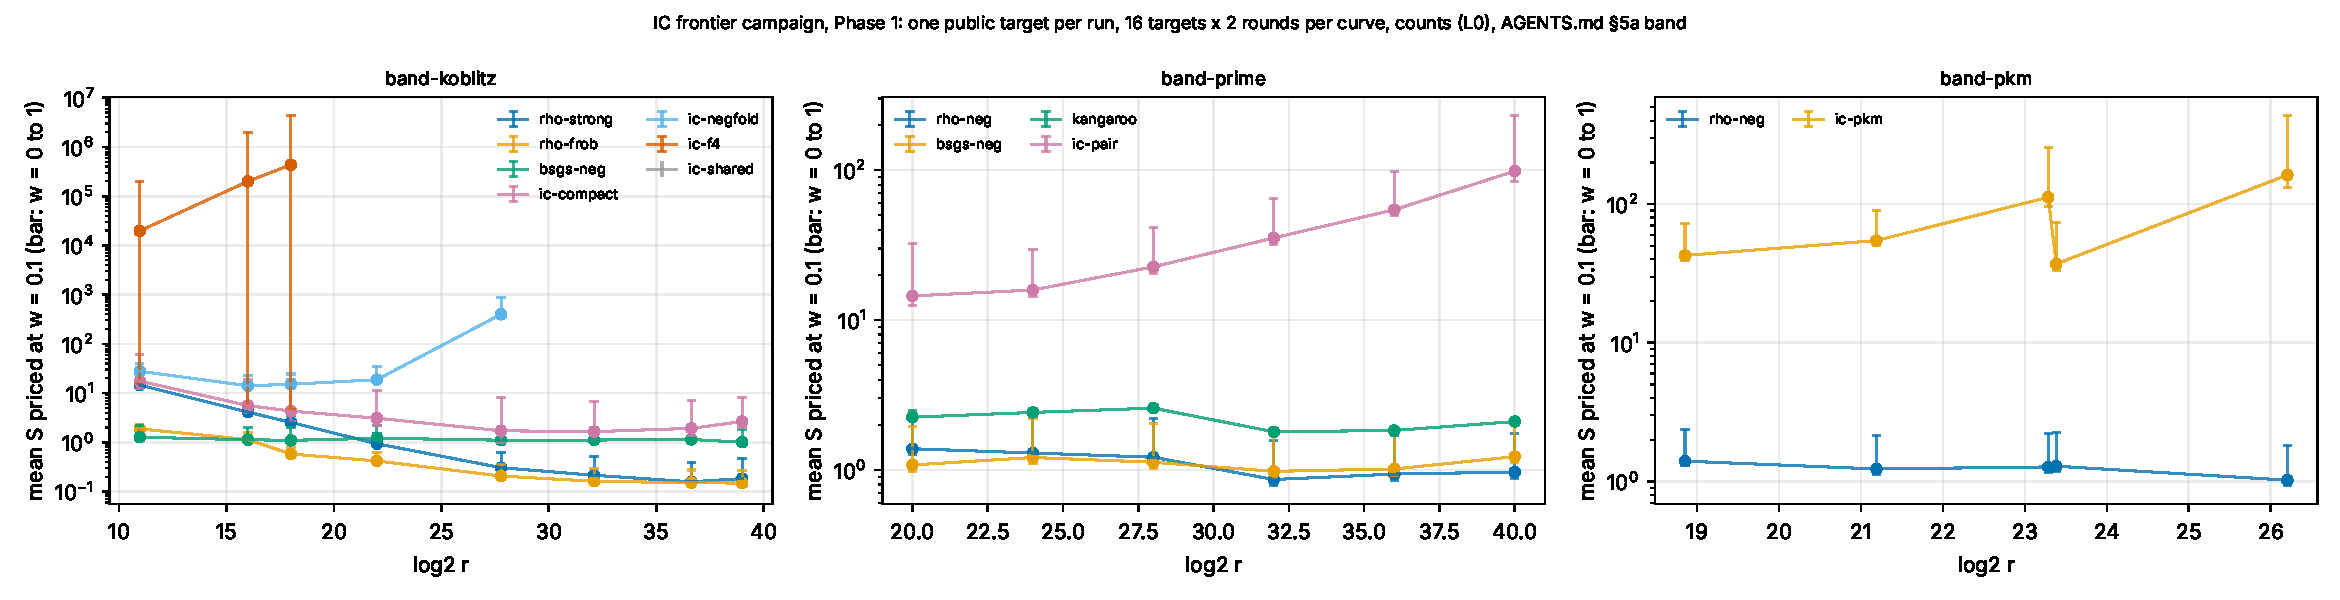
\includegraphics[width=\linewidth]{figures/fig-campaign.pdf}
\caption[]{The campaign frontier: mean $S$ per arm and curve at $w=0.1$ GAE
per native operation, the bar spanning $w=0$ to $w=1$; one public target
per run, 16 targets $\times$ 2 rounds per curve, operation counts.
Sources: \art{research/ic_frontier_campaign_20261015/analysis/band-*.json}
(\texttt{ecbench band}).}
\label{fig:campaign}
\end{figure}

\begin{table}[t]
\centering\small
\caption[]{Index calculus over the cheapest constant-memory generic arm on
the same curve (signed-Frobenius rho on Koblitz curves, rho with negation
on prime curves), mean $S$ ratio at three band weights. Every run verified
(32/32 per cell). Source:
\art{research/ic_frontier_campaign_20261015/analysis/ratios_to_rho.tsv}.}
\label{tab:campaign}
\begin{tabular}{@{}lrlrrr@{}}
\toprule
Curve & $\log_2 r$ & Arm & $w=0$ & $w=0.1$ & $w=1$ \\
\midrule
Koblitz $n=13$ & 11.0 & compact orbit & 6.9 & 9.3 & 27.1 \\
               &      & negfold       & 14.4 & 14.8 & 17.5 \\
Koblitz $n=17$ & 16.0 & compact orbit & 3.8 & 4.9 & 11.8 \\
Koblitz $n=19$ & 18.0 & compact orbit & 4.9 & 7.5 & 23.6 \\
Koblitz $n=23$ & 22.0 & compact orbit & 5.5 & 7.4 & 18.4 \\
Koblitz $n=37$ & 27.8 & compact orbit & 5.2 & 8.3 & 23.3 \\
               &      & negfold       & 1806 & 1927 & 2512 \\
Koblitz $n=43$ & 32.1 & compact orbit & 7.4 & 10.2 & 23.1 \\
Koblitz $n=47$ & 36.6 & compact orbit & 9.9 & 12.7 & 25.3 \\
Koblitz $n=41$ & 39.0 & compact orbit & 15.0 & 17.8 & 30.3 \\
\addlinespace
prime 20 bit & 20 & pair table & 9.8 & 10.5 & 13.5 \\
prime 24 bit & 24 & pair table & 12.1 & 12.2 & 12.9 \\
prime 28 bit & 28 & pair table & 18.6 & 18.6 & 18.9 \\
prime 32 bit & 32 & pair table & 40.9 & 40.9 & 41.1 \\
prime 36 bit & 36 & pair table & 58.1 & 58.0 & 57.5 \\
prime 40 bit & 40 & pair table & 95.2 & 101.8 & 131.4 \\
\addlinespace
PKM 20 bit & 18.9 & Kummer tower & 30.3 & 30.4 & 31.0 \\
PKM 28 bit & 26.2 & Kummer tower & 141.3 & 158.7 & 238.7 \\
\bottomrule
\end{tabular}
\end{table}

\paragraph{What the campaign shows.}
\begin{itemize}
\item \emph{No index-calculus arm beats generic rho on any curve, at any
  weight.} Signed-Frobenius rho is below every index-calculus arm on all
  eight Koblitz curves and across the whole band; rho with negation is
  below every prime-field arm on all eleven prime curves
  (Table~\ref{tab:campaign}). The one unresolved pair in the campaign is
  compact orbit against the \emph{strong} rho reference at $n=13$, whose
  scalar-multiplication set-up dominates on an 11-bit subgroup; the
  cheaper signed-Frobenius walk is below both.
\item \emph{Compact orbit is the closest index calculus.} It sits
  $3.8$--$15\times$ the best rho with native work free and
  $4.9$--$17.8\times$ at $w=0.1$; the ratio does not shrink with size.
\item \emph{Prime-field index calculus falls further behind with size.}
  The two-summand pair-table arm goes from $10.5\times$ to $101.8\times$
  rho (at $w=0.1$) between 20 and 40 bits, the $r^{1/6}$ widening its
  $r^{2/3}$ cost against rho's $r^{1/2}$ predicts; the Kummer-tower arm is
  $28$--$159\times$ rho.
\item \emph{Negfold root finding stops scaling.} It is $12$--$45\times$
  rho up to $n=23$, about $1{,}900\times$ at $n=37$, and does not complete
  within $5\cdot10^7$ trials from $n=43$ on (PROTOCOL A4b).
\item \emph{Inherited F4 is not competitive once its work is priced}:
  $S$ rises from $16$ (word XORs free) to about $2\cdot10^4$ at
  $w=0.1$ at $n=13$. The band weighs one 64-bit word XOR like a table
  lookup, which overstates F4 (its pinned calibration is about
  $0.002$ GAE per XOR); even with XORs free it is above rho.
\item \emph{BSGS has the lowest time on several curves} because it spends
  $\sqrt r$ memory; it is reported on the time--memory Pareto set, not
  ranked against constant-memory methods.
\end{itemize}

\paragraph{Cost exponents.} Fitting total cost $\propto r^{\alpha}$ per
arm over each size tier with \texttt{ecbench bound fit --weight}
(two-stage bootstrap, 95\% intervals; a tier needs at least four sizes for
an exponent):
\begin{itemize}
\item prime pair table $\alpha=0.620$ $[0.557,0.663]$ at $w=0$ against
  rho with negation $0.435$ $[0.331,0.501]$; separated at $w=0$ and
  $w=0.1$, overlapping at $w=1$ ($0.594$ $[0.482,0.665]$ against $0.444$
  $[0.334,0.517]$). Index calculus grows faster than rho (the predicted
  $2/3$ against $1/2$), but under the band rule the difference is not
  established at every weight;
\item Koblitz compact orbit, $n=37$--$47$: $0.589$ $[0.518,0.743]$ against
  signed-Frobenius rho $0.436$ $[0.358,0.508]$ at $w=0$, overlapping at
  $w=0.1$ and $w=1$; on $n=13$--$23$ the two overlap at every weight
  ($0.25$ against $0.29$ at $w=0$, both with wide intervals because the
  automorphism count $2n$ changes with the size);
\item Kummer tower $0.717$ $[0.358,0.940]$ against $0.438$
  $[0.332,0.599]$, overlapping.
\end{itemize}
No index-calculus arm has a fitted exponent below rho's at any weight, so
no crossover with rho is supported by these data, extrapolated or
otherwise. The fitted rho exponents ($0.435$--$0.444$) lie below the
theoretical $1/2$, which reads as a toy-size effect (fixed per-run overheads
and the size-dependent automorphism count) rather than a property of rho; so
the measured widening of the gap is a fit on small sizes, and the conclusion
that it widens as $r^{1/6}$ rests on the generic-oracle bound, not on these
fits alone. The sixty-three fits are in
\art{research/ic_frontier_campaign_20261015/analysis/bounds/}.

\paragraph{Limits.} Operation counts only (isolation L0); wall time and a
second-host replay certificate need the planned RunPod phase. Parameters
were selected on four training targets per size. The shared-rank arm
leaves three categories of work uncounted and is reported as a lower
bound only. Fitted cost exponents per arm and tier are in
\art{research/ic_frontier_campaign_20261015/analysis/bounds/}.

\section{The engineering record}

Table~\ref{tab:improvements} collects the measured improvements of the
programme on the boundary each was measured on. Ratios are
baseline/candidate; ``stage'' means one oracle call or one solver run;
``complete'' means a verified discrete logarithm with the stated phases.

\begin{table}[p]
\centering\small
\caption[]{Measured improvements, July--October 2026. Class: E =
\cls{engineering}, A = \cls{accounting}. Boundary: St = stage,
Cx = complete solve outside ecbench, Cold = ecbench cold one-target $S$,
On = online window after retained set-up. Sources: Appendix~\ref{app:artefacts}.}
\label{tab:improvements}
\begin{tabularx}{\linewidth}{@{}>{\raggedright}Xllr>{\raggedright\arraybackslash}p{3.0cm}@{}}
\toprule
Change & Bnd. & Cl. & Ratio & Scope \\
\midrule
\multicolumn{5}{@{}l}{\emph{Decomposition oracle: root finding}}\\
$\Sem3$ roots, binary pair table vs matrix F4 & St & E & $383$--$1{,}535$ & $\FF_{2^9}$, $\FF_{2^{13}}$, $m=2$ \\
$\Sem3$ roots, prime vs \texttt{groebner\_f4} & St & E & $3.5$--$4.7{\cdot}10^4$ & 16--24-bit, $\abs\Fb=6$ \\
$\Sem3$ roots vs Buchberger, NIST curves & St & E & $3{,}021$--$5{,}802$ & P-192\ldots P-521 \\
\texttt{rf-mitm} vs PS-0 oracle & St & E & $3{,}007$--$115{,}160$ & binary $\ell=8..14$ \\
Root-finding DLP vs msolve DLP & Cx & E & $50$--$105$ & 16--24-bit prime \\
Pair-table DLP vs F4 DLP & Cx & E & $122$ & binary $n=23$ (F4 wins $n\le13$) \\
Pair table vs subtraction & Cold & E & $53.0$ & 20-bit prime (bounded) \\
Frobenius pair table vs subtraction & Cold & E & $17.5$ & Koblitz $n=17$, priced \\
Root-finding K13 arm, first to best & Cold & E & $1.69$ & $38.82\to22.97$, across sessions \\
Windowed $m=3$ scan & Cold & E & $1.21$ & $[1.16,1.28]$ \\
Negfold root finding vs XOR-priced F4 & Cold & E & $18.3$ & $[15.6,21.3]$, K13 \\
Dense root index K1798 vs K1500 (probes) & On & E & $1.77$ & $n=83$, one point \\
Pair-table size 64 vs 32 abscissae & Cold & E & $1.20$ & $[1.04,1.43]$ \\
\addlinespace
\multicolumn{5}{@{}l}{\emph{Gr\"obner engines}}\\
Inherited vs matrix F4 (matrix work) & St & E & $198.6$--$222.1$ & K13, R13 \\
F5 vs matrix F4 (word XORs) & St & E & $1.55$--$1.56$ & K13, R13 \\
F6-IC vs inherited F4 (word XORs) & St & E & $1.22$--$1.30$ & $m=13,19$ \\
\texttt{f4\_fp} new vs previous & St & E & $29.8$--$54.1$ & square systems, = msolve \\
Four-Russians routing & St & E & $1.75$--$3.22$ & oracle matrices \\
Eager vs lazy inherited rewrite & St & E & $1.40$--$1.62$ & dim 8--9 \\
Quotient-curve $m=2$ model & St & E & $1.34$--$1.64$ & five cells \\
\addlinespace
\multicolumn{5}{@{}l}{\emph{Factor bases and symmetry}}\\
Compact orbit vs full orbit & Cold & E & $\le1.87$ & Koblitz $n=17$; compact is LB \\
FGHR $D_4$ vs Gaudry $S_4$, $C_4$ & St & E & $47.5$--$48.4$ & $\FF_{269^4}$ \\
\texttt{gaudry\_quartic} solve & St & E & $1.96$--$6.08$ & $d=4..6$ (sweep recompute) \\
\addlinespace
\multicolumn{5}{@{}l}{\emph{One-target online}}\\
Compact-orbit IC vs strong rho & On & E & $13.94$ & $n=61$; rho without a table; retired (\S\ref{sec:ladder}) \\
\addlinespace
\multicolumn{5}{@{}l}{\emph{Accounting (costs that went up when priced)}}\\
F4 word XORs priced & Cold & A & $1/25.2$ & $16.75\to421.4$, K13 \\
F6-IC batched geometry priced & Cold & A & $1/64.6$--$1/1{,}353$ & $m=13,19$; F4 unpriced (about $1/2.5$ priced) \\
\bottomrule
\end{tabularx}
\end{table}

\noindent Derived entries: $53.0=1/0.018861$; $17.5=1/0.057047$;
$1.21=1/0.828$ with interval from $[0.783,0.863]$; $18.3=1/0.0545$ with
interval from $[0.047,0.064]$; $1.77=300{,}021.9/169{,}069.8$; $1.20=1/0.830$
with interval from $[0.697,0.962]$; $1.87=18.714/9.985$ (one session; the compact arm's $S$ is a lower bound, so
the ratio is an upper bound); $1.69$ and $25.2$ compare means from different
sessions with different seeds and are descriptive; F5 and F6-IC ratios are
reciprocals of the recorded candidate/baseline word-XOR ratios.

\section{The improvement ladder, 14--15 October}\label{sec:ladder}

The repository's owner fixed the criterion for success on 15 October: a
verified, measured improvement over the current index-calculus baseline is
a success; each one becomes the new baseline; the gap to the matched rho is
reported as the distance remaining, not as a pass/fail gate; and
relabelling or accounting changes do not count. In the two days before
that, two improvement rounds and a next-steps campaign landed about twenty
measured changes, each paired against its own incumbent under a protocol
frozen before data. Figure~\ref{fig:ladder} and Table~\ref{tab:ladder}
list them, with the distance to rho that remains after each one.
None is in the frontier campaign of \S\ref{sec:campaign}, which predates
them, and none was priced across the band; the boundaries are the ones the
studies used, which differ from row to row.

\begin{figure}[t]
\centering
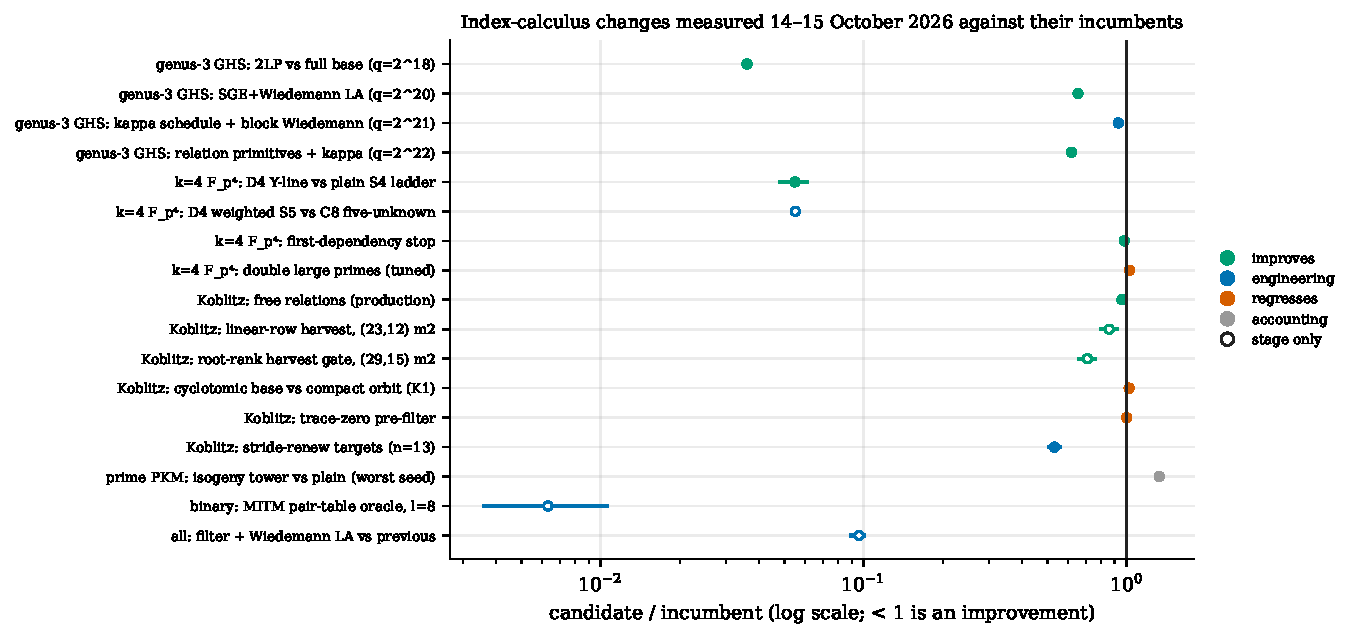
\includegraphics[width=\linewidth]{figures/fig-ladder.pdf}
\caption[]{Candidate over incumbent for the changes of 14--15 October, with
95\% intervals where the study reports one (the binary oracle's range is
the spread over three runs). Filled: whole solve; open: one stage. Values:
\art{papers/ecdlp-index-calculus-program/figures/ladder.tsv}; sources in
Table~\ref{tab:ladder}.}
\label{fig:ladder}
\end{figure}

\begin{table}[p]
\centering\small
\caption[]{Changes measured 14--15 October 2026 against their own
incumbents. Ratio: candidate/incumbent, $<1$ better. Class, against the
index-calculus incumbent (not the paper's \cls{advance}, which is against
rho): Ie = improves the exponent, Ic = improves the constant, E =
\cls{engineering} on one stage, R = regresses, T = trades, A =
\cls{accounting}. ``To rho'':
the distance left to the matched rho on the study's own boundary; ``d'' marks
a derived or extrapolated value. Sources under \art{research/}:
\texttt{ic\_next10\_20261014/}, \texttt{ic\_improve\_20261014/},
\texttt{ic\_improve\_20261015/}, \texttt{ic\_improve3\_20261015/} and the
named study directories.}
\label{tab:ladder}
\begin{tabularx}{\linewidth}{@{}>{\raggedright}Xl>{\raggedright}p{3.6cm}>{\raggedright\arraybackslash}p{3.2cm}@{}}
\toprule
Change & Cl. & Ratio [95\%] & To rho \\
\midrule
\multicolumn{4}{@{}l}{\emph{Genus 3 after the cubic GHS transfer, $E_0(\FF_{q^3})$, cost in $\FF_q$ multiplications}}\\
Double large primes vs full base (04) & Ie & $0.036$ $[0.035,0.036]$ at $2^{18}$; $q^{1.910}\to q^{1.385}$ & $2.58\times$ negation rho model at $q=2^{20}$ \\
Large primes as columns, SGE, Wiedemann (01) & Ie & $0.653$ $[0.647,0.660]$ at $2^{20}$; $q^{1.398}\to q^{1.380}$ & --- \\
$\kappa(q)$ schedule + block Wiedemann (06) & T & $0.929$ at $2^{21}$ & $1.15\times$ measured negation rho at $2^{20}$ (ref.) \\
Cheaper relation primitives + re-tuned $\kappa$ (r3-01) & Ic & $0.617$ $[0.616,0.619]$ at $2^{22}$ & no matched rho in this unit \\
\addlinespace
\multicolumn{4}{@{}l}{\emph{$k=4$ over $\FF_{p^4}$, operation counts}}\\
$D_4$ $Y$-line vs plain $\Sem4$, $p=101$--$1033$ & Ic & $0.0548$ $[0.048,0.061]$ & handover $2^{126}$--$2^{137}$ (d) \\
$D_4$-weighted $\Sem5$, four unknowns, vs five & E & $1/18.5$--$1/17.8$ & handover $2^{135.6}\to2^{118.9}$ (d) \\
First-dependency stop (\texttt{d4-ed}) & Ic & $0.979$ $[0.973,0.986]$ & no $k=4$ run below rho \\
Double large primes, tuned & R & $1.025$ $[1.016,1.037]$ (LA $0.827$) & --- \\
\addlinespace
\multicolumn{4}{@{}l}{\emph{Koblitz, compact orbit and Gr\"obner oracle}}\\
Free relations in production, $n=41,53,61$ & Ic & $0.960$ $[0.946,0.976]$ & $3.8$--$15\times$ rho-frob ($w=0$, \S\ref{sec:campaign}) \\
Linear-row harvest, $(23,12)$, $m=2$ & Ic & $0.858$ $[0.803,0.916]$ & oracle stage; default on \\
Root-rank harvest gate, $(29,15)$, $m=2$ & Ic & $1/1.41$ $[1/1.52,1/1.32]$; end to end $1/1.20$ & oracle stage; default on \\
Gated fall-row augmentation & Ic & $1/11.9$ on barrel $n=13$; $1$ in production & production no-op \\
Equivariant Macaulay oracle & T & $4.0$ ($n=5$) \ldots\ $1/15.5$ ($n=13$) & not applicable to production \\
\texttt{stride-renew} targets, $n=13$ & E & $0.531$ $[0.506,0.557]$ & $4.7\times$ rho-strong at $n=19$ \\
Cyclotomic $\gamma$-weight base, K1 & R & $1.022$ $[1.021,1.023]$ & yield-neutral \\
Trace-zero pre-filter & R & $1.00003$ & vacuous on odd order \\
\addlinespace
\multicolumn{4}{@{}l}{\emph{Prime fields and shared stages}}\\
PKM isogeny tower, search charged & A & $1.002$--$1.331$ & $17$--$137\times$ rho \\
Binary MITM pair-table oracle, $\ell=8$ & E & $1/277$--$1/94$ per target & no exponent claim \\
Filter + Wiedemann LA, $D=2^{18}$ & E & $1/10.40$; $1/1.93$ vs CADO-NFS & LA is 0.1--1.9\% of runs \\
\bottomrule
\end{tabularx}
\end{table}

\paragraph{Genus three: an exponent below rho's.} The cubic GHS
transfer~\cite{ghs2002} maps the DLP in $E_0(\FF_{q^3})$ to the Jacobian
of a genus-3 hyperelliptic curve over $\FF_q$, where double-large-prime
index calculus~\cite{gtthd2007} costs $\tilde O(q^{2-2/g})=\tilde O(q^{4/3})$
against rho's $q^{3/2}$. That is known; what is new is a priced,
end-to-end, verified run of it on a family the repository can build
($4\mid\#E_0(\FF_{q^3})$, split arm, $q=2^{8}$--$2^{22}$, every logarithm checked
against the planted scalar). Adding double large primes changed the
exponent from $q^{1.910}$ to $q^{1.385}$ $[1.379,1.391]$, and keeping the large
primes as columns, merging them with structured Gaussian elimination and
finishing with Wiedemann moved it to $q^{1.380}$ and the constant to
$0.653\times$. This was the first index-calculus family in the programme whose fitted
exponent lies below rho's (the $k=4$ binary family of \S\ref{sec:ladder2}
is the second), and the only one where measured IC beats a rho arm: the item-7 rho, which walks at $1.75\sqrt\ell$ steps,
at $q=2^{15}$ ($0.69$ $[0.55,0.83]$). Two further
rounds kept going. A frozen schedule for the factor-base fraction $\kappa(q)$
plus block Wiedemann brought the whole solve to $0.605\times$ the first
double-large-prime arm at $q=2^{21}$. Cheaper relation primitives
(one-inversion Cantor addition, a Stickelberger pre-filter, reused
exponentiations) then cut the relation phase to $0.47\times$ without
changing a single relation, and with $\kappa$ re-tuned the whole solve to
$0.617$ $[0.616,0.619]$ at $q=2^{22}$, in a unit that also charges
inversions. The distance to rho shrank from $2.58\times$ the negation-map
rho model at $q=2^{20}$ (first double-large-prime arm) to $1.15\times$ a
measured negation-map rho there after the second round ($2.31\cdot10^{10}$
against $2.01\cdot10^{10}$ $\FF_q$ multiplications; a reference on
overlapping but not identical curves). The third round's $0.62\times$
has no matched rho in its unit yet, so whether it crosses is not
established. The local exponents sit at $1.38$--$1.41$, still above $4/3$,
because the linear algebra grows faster than $q^{4/3}$ and the tuned
$\kappa$ falls with $q$. The family is narrow: the transfer needs the
right 2-power torsion, and $\FF_{q^3}$ curves are not deployed.
\emph{Next improvement}: a negation-map rho measured in the third round's
unit on the same instances, then the run past $q=2^{22}$ that would show a
crossover or rule it out.

\paragraph{The $k=4$ chain.} The $D_4$ Macaulay system of
\S\ref{sec:gaudry} entered a complete ladder ($p=101$--$1033$, 21 curves):
$18.2\times$ cheaper than plain $\Sem4$ at the same exponent, with the
handover with negation rho extrapolated to $2^{126}$--$2^{137}$. Writing
the $D_4$-symmetrised $\Sem5$ in four weighted unknowns cut the per-solve
cost another $17.8$--$18.5\times$, to $1.42\cdot10^9$ $\FF_p$
multiplications, $854\times$ below the plain form; in the 2-torsion frame
that moves the derived handover from $2^{157.9}$ to $2^{118.9}$. Double
large primes cut the linear algebra ($0.827\times$) but regress the whole
solve; stopping at the first dependency gains $2.1\%$. No $k=4$ run below
rho exists; every handover is an extrapolation of fitted exponents through
a measured constant. \emph{Next improvement}: put the four-unknown solve
into the complete ladder, then keep double large primes' linear-algebra
gain without its relation-phase cost.

\paragraph{Koblitz.} Free relations---root-table self-collisions used as
homogeneous rows---are now the production default ($0.960\times$ counted,
$0.941\times$ wall); the linear rows the Gr\"obner oracle used to discard
are harvested ($0.86$--$0.93\times$ where the gate fires, and a root-rank
gate then made it fire on more cells: $1/1.41$ at $(29,15)$, $1/1.20$ end
to end); the gated
fall-row and equivariant passes pay only on overdetermined systems the
production pipeline does not build. The cyclotomic base and the trace-zero
filter were refuted. A census closes the free-relation lever at the rungs
run: at $n=61$, $K=600$ the self-collisions span 49 independent relations of
the 599 needed, and full rank would need $K\approx2{,}050$. The distance to
signed-Frobenius rho is still $3.8$--$15\times$ cold at $w=0$, and the
fitted Koblitz ratio grows as about $r^{1/6}$ (slope $0.165$ $[0.117,0.213]$
per $\ln r$ on eight public curves, every native priced).
\emph{Next improvement}: relation yield per probe, which none of these
changes touched.

\paragraph{The online result is retired.} An equal-advice audit
gave Bernstein--Lange preprocessing rho~\cite{bl2012} a distinguished-point
table no larger than the index-calculus pair table and ran both on the same
64 unseen targets at $n=41$, 53 and 61. Rho with the table is $53$--$317\times$
faster online (at $n=41$, with exactly equal advice, $317$ $[137,739]$), and
even at $1/1{,}024$ of the bytes it stays $7.7$--$32\times$ faster. The
$13.9\times$ online win of \S\ref{sec:koblitz} and the later $7.3\times$ and
$12.3\times$ hosted single-target points at $n=71$ and $n=83$ compared
index calculus \emph{with} a table against rho \emph{without} one. They are
measurements of the preprocessing model, not index-calculus improvements,
and the online frontier belongs to preprocessing rho.

\paragraph{The reference moved too.} Two rho studies shortened the
distances above. On prime curves, choosing the better of $P+R$ and $P-R$
at each step takes $1.129\times$ fewer steps under distinguished points
($1.081$--$1.184$); each step costs more, so the predicted net gain is
$1.03$--$1.12\times$ with 8--64 walks per inversion and a net loss ($0.95$)
at 1{,}024. On ECC2K-130, signed $\sigma$ steps cut GPU time per
solve to $0.961$--$0.970$ (derived; not rolled out). Neither is yet in a
campaign arm. A comparison against a rho that has not adopted them would
overstate index calculus's position by that much.

\section{The ladder continued, 16--20 October}\label{sec:ladder2}

Work that reached \texttt{main} between 16 and 20 October, after the programme record
was first assembled (some of it measured on 14--15 October), added a
genus-3 round, two $k=4$ oracles, a long binary-oracle ladder, Gr\"obner-engine work and a
repository-wide validation sweep (Figure~\ref{fig:ladder2},
Table~\ref{tab:ladder2}). The reading rules of \S\ref{sec:ladder} apply:
each row is against its own incumbent, on its study's boundary, unpriced
across the band.

\begin{figure}[t]
\centering
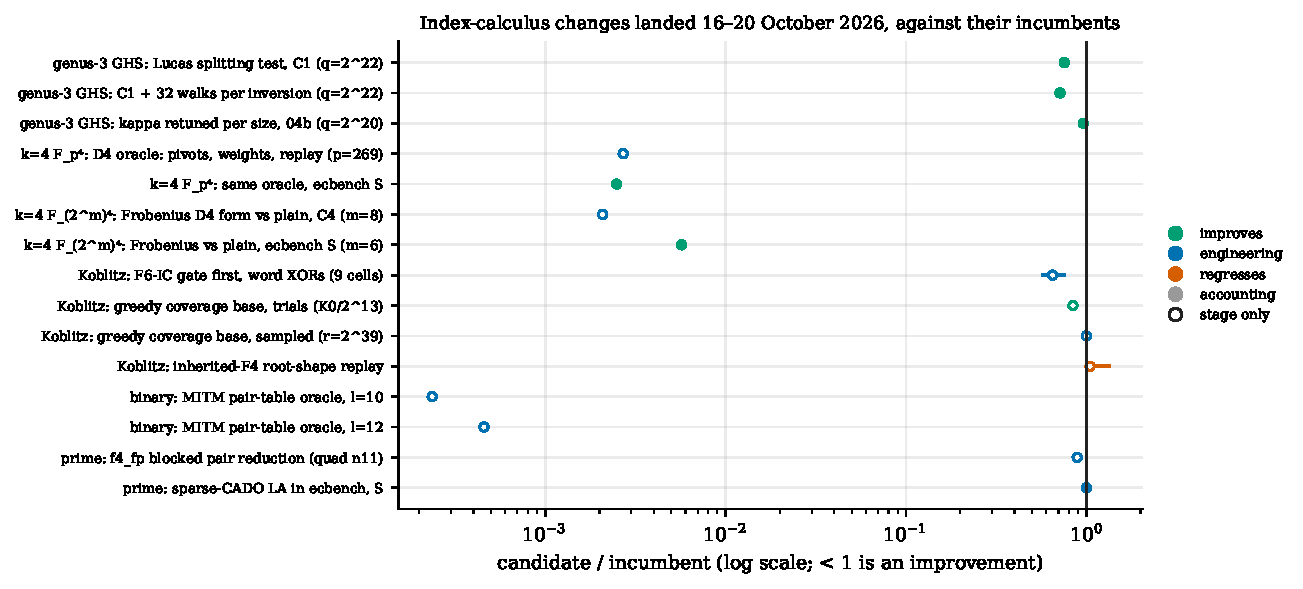
\includegraphics[width=\linewidth]{figures/fig-ladder2.pdf}
\caption[]{Candidate over incumbent for the changes that landed 16--20 October, as in
Figure~\ref{fig:ladder}. Values:
\art{papers/ecdlp-index-calculus-program/figures/ladder2.tsv}; sources in
Table~\ref{tab:ladder2}.}
\label{fig:ladder2}
\end{figure}

\begin{table}[p]
\centering\small
\caption[]{Changes that landed 16--20 October 2026, against their own
incumbents; columns and classes as in Table~\ref{tab:ladder}. Sources under
\art{research/}: \texttt{ic\_improve4\_20261015/},
\texttt{ic\_improve\_20261014/04b-genus3-2lp-rebalance/},
\texttt{gaudry\_quartic\_d4\_cost\_20261014/},
\texttt{gaudry\_quartic\_d4\_char2\_20261015/},
\texttt{joux\_vitse\_n1\_20261015/}, \texttt{binary\_mitm\_oracle\_l9\_l10\_20261015/},
\texttt{binary\_mitm\_oracle\_l11\_l12\_20261016/},
\texttt{ic\_m3\_algebraic\_vs\_mitm\_20261014/}, \texttt{secg\_small\_x\_20261014/},
\texttt{greedy\_factor\_base\_yield\_20261014/}, \texttt{f6\_gate\_first\_x86\_20261016/},
\texttt{pdp\_shape\_replay\_20261015/}, \texttt{f4\_fp\_blocked\_pairs\_20261016/},
\texttt{ic\_linalg\_pipeline\_20261019/}, \texttt{k\_conversion\_20261018/}.}
\label{tab:ladder2}
\begin{tabularx}{\linewidth}{@{}>{\raggedright}Xl>{\raggedright}p{3.6cm}>{\raggedright\arraybackslash}p{3.2cm}@{}}
\toprule
Change & Cl. & Ratio [95\%] & To rho \\
\midrule
\multicolumn{4}{@{}l}{\emph{Genus 3 after the cubic GHS transfer}}\\
Lucas splitting test (round 4, C1) & Ie & $0.756$ $[0.755,0.756]$ at $2^{22}$; local $1.408\to1.364$ & no rho arm since round 2 \\
C1 + 32 walks per inversion & Ic & $0.715$ at $2^{22}$; local $1.356$ & as above \\
Factor base retuned per size (04b) & Ic & $0.961$ at $2^{20}$ & $0.16\times$ rho on $\mathrm{Jac}(C)$ at $2^{14}$, not on $E_0$ \\
\addlinespace
\multicolumn{4}{@{}l}{\emph{$k=4$ over $\FF_{p^4}$ and $\FF_{(2^m)^4}$}}\\
$D_4$ oracle: pivots, weighted form, replay, $p=269$ & E & $1/370$ $[1/371.6,1/367.9]$ & --- \\
Same oracle, ecbench $S$ & Ic & $1/402$ $[1/406,1/398]$ & $1.39\cdot10^6\times$ rho \\
Frobenius-reduced $D_4$ form, characteristic 2, $m=8$ & E & $1/481$ $[1/483,1/479]$ & --- \\
Same, ecbench $S$ ($m=6$) & Ic & $0.0057$ & $6.1\times$ rho model, $4.3\times$ measured, at $n\approx2^{56}$ \\
\addlinespace
\multicolumn{4}{@{}l}{\emph{Koblitz and binary oracles}}\\
F6-IC gate-first order & E & $1/1.73$--$1/1.34$ word XORs & default on \\
Greedy coverage base, $K_0/2^{13}$ & Ic & $0.843$ (expected trials) & gain $1.000$ at $r=2^{39}$ \\
Inherited-F4 root-shape replay & R & $1.015$--$1.328$ & switch stays off \\
Binary MITM oracle, $\ell=9..12$ & E & $1/4{,}244$--$1/928$ per target & relation collection $\Theta(2^n)$ \\
Algebraic $m=3,4$ oracles vs MITM floor & R & slope $0.53$--$0.81$ vs $0.21$--$0.36$ & $3\cdot10^2$--$3\cdot10^4\times$ floor \\
\addlinespace
\multicolumn{4}{@{}l}{\emph{Prime fields and shared stages}}\\
\texttt{f4\_fp} blocked pair reduction & E & $0.78$--$0.89$ (wall, quad $n10,11$) & beats msolve there \\
Sparse-CADO LA inside ecbench & E & $S$ $1.000$; LA wall $0.25$--$0.72$ & $149\times$ rho \\
$S_3$ solve on SECG small-$x$ bases & --- & table $2{,}600$--$313{,}000\times$ cheaper & $52$--$280$ bits over rho \\
Column-touch conversion $K$ (ECC2K-130 $m=4$) & A & $+7.62/+10.32\to+9.78/+12.48$ bits ($w=1$ floor; $+45.71$ at $w=2$, unconverted) & accounting \\
\bottomrule
\end{tabularx}
\end{table}

\paragraph{Genus three, round four.} A field-level splitting test (a Lucas
ladder on the Cardano resolvent's cubic character, with the same relations)
removes most of the per-trial log factor (9.75 to 2.71 units per bit) and
moves the whole solve to $0.756\times$ at $q=2^{22}$; with 32 walks sharing
one inversion, to $0.715\times$, with local exponent $1.356$ (fitted
$1.368$ over $2^{16}$--$2^{22}$), $0.023$ above $4/3$. Chained with round
three, the whole solve is about $0.44\times$ the second round's at
$q=2^{22}$ (derived, in the inversion-charging unit). Rounds three and four
ran no rho arm; a 23 October study then measured round 4 against the
strongest rho at $q=2^{14}$--$2^{20}$: under the registered pricing it is
below rho at $2^{16}$ at every band weight and unresolved at the other
sizes (geometric means $0.70$--$1.52$), and above rho under the protocol's
heavier sensitivity pricing; \S\ref{sec:transfer}). Re-tuning $\kappa$ on training again steepened the schedule
and raised the exponent. A separate rebalance study measured IC at
$0.16\times$ ($0.25\times$ renormalised) a rho on $\mathrm{Jac}(C)$ at
$q=2^{14}$: that rho walks on the Jacobian (four walks per size, at
$1.6$--$2.8$ steps per $\sqrt\ell$ against an ideal $1.25$), not on
$E_0(\FF_{q^3})$, so it is not the matched reference and the ratio is not
a distance to rho.
Memory now limits the ladder: $q=2^{22}$ peaks at 3.9\,GB of a 4.5\,GB cap.

\paragraph{$k=4$: two oracles and a closing gap.} Over $\FF_{p^4}$, sparsest
pivots, the weighted grading $\sigma_4=\pi^2$ and shape replay cut one $D_4$
decomposition from $2.55\cdot10^{10}$ to $6.89\cdot10^7$ $\FF_p$
multiplications ($370\times$; 648/648 solves exact) and ecbench $S$ by
$398$--$406\times$; index calculus is still $1.39\cdot10^6\times$ rho at
the measured sizes and the model handover moves from $2^{135}$ to $2^{103}$.
In characteristic two, a Frobenius-reduced form of the same system
(weights $(2,2,1,1)$, Macaulay degree 11, a $384\times448$ matrix) is
$481\times$ below the plain form. End to end on $E(\FF_{(2^m)^4})$ the
ratio of IC to the negation-map rho model falls from $5{,}080$ at $m=6$ to
$6.06$ at $m=14$ ($n\approx2^{56}$; $4.3\times$ a measured rho), with fitted
slope $-0.248$ in $\log_2 n$---Gaudry's $n^{-1/4}$---and an extrapolated
crossover near $n\approx2^{68}$ ($2^{63}$--$2^{69}$ under the model).
After genus three, this is the nearest any index calculus in the programme
has come to rho, and its extrapolated crossover lies where rho itself takes
about $2^{34}$ steps, so the extrapolation can be tested directly. A Joux--Vitse
$(n-1)$-decomposition at $n=5$ on $E(\FF_{p^5})$ completed verified DLPs at
$4.5\cdot10^7$--$1.8\cdot10^8\times$ rho, with a crossover extrapolated to
groups near $2^{291}$.

\paragraph{Binary oracles and their floor.} The MITM pair-table oracle on a
non-Koblitz curve reached $\ell=12$ over $\FF_{2^{37}}$
($2{,}474$--$4{,}244\times$ over pairs-and-solve at $\ell=9,10$;
$928$--$2{,}321\times$ at $\ell=11,12$, the last as recomputed by the
validation sweep; 0 disagreements on 256 targets).
Against that floor, no algebraic oracle (inherited F4, F6-IC, SAT, split
$\Sem4$ hybrids, a wide chained $\Sem3$ solver) grows more slowly in $n$:
the cheapest is $3\cdot10^2\times$ the floor at $n=13$ and $3.8\cdot10^4\times$
at $n=31$ for $m=3$, and the $m=4$ chain grows at slope $0.805$ against the
floor's $0.333$. A greedy coverage base needs $1.08$--$1.18\times$ fewer
trials on small Koblitz curves, but its gain falls to $1.0000$ at
$r=2^{39}$. On the 33 SECG curves an $\Sem3$ solve over a small-$x$ base,
with no table, is $52$--$280$ bits over rho.

\paragraph{The reference moved again.} The strong signed-Frobenius rho of
every Koblitz comparison executed 718 instructions per walk step after
three rounds, down from 1{,}196; a fourth round of batched inversion took
main from $707.2$ to $679.7$ Callgrind instructions per step at $n=53$, with
no established native-time gain (outputs identical;
\art{research/rho_batchinv_20261022/}; steps per ideal
$0.92$--$0.99$ on 400 fixtures), and ecbench's standing
\texttt{rho.signed\_frobenius\_strong} runs at $0.802\times$ its former
instruction count with identical GAE. On hyperelliptic Jacobians the
programme's rho was slow at large $N$ until full-width branch coefficients
brought $S_\text{walk}$ from $2.10$ to $1.48$; the negation fold saves only
$0.97\times$ at $N\ge10^5$. Counted-unit comparisons ($S$) are unaffected
by the instruction counts; wall-time comparisons against the older rho
overstate index calculus by up to the same factor.

\paragraph{Corrections from the validation sweep.} A repository-wide
validation sweep (19--20 October) contradicted five recorded results, all
now struck through in their sources with dated notes. Three bear on this
paper. (i) The one-point $n=83$ online ratio ($18.5\times$,
\S\ref{sec:rootfinding}) and the hosted $n=71$/$n=83$ panels ($7.3\times$,
$12.3\times$) compared against rho with an empty table; with a
Bernstein--Lange table matched to the index calculus's set-up time or
memory, precomputed rho is faster in every matched $n=83$ pair
($3.7\times$ time-matched and $40.6\times$ memory-matched against $K=3300$;
$82$--$396\times$ against $K=600$). They join the $n=61$ point as retired.
(ii) The root-finder session's replay-all, recorded as 120/168 identical with
the 48 mismatches confined to inherited F4, replays 72/168 on current
\texttt{main}, with mismatches in all four IC arms, root finding included.
The sweep later isolated the cause: an x86-only BMI2 rewrite in inherited F4
charges a different word-XOR count from the portable path, and with it
disabled x86 and emulated aarch64 both replay 168/168
(\art{research/validation_sweep_20261019/D-known-issues/item1_cross_isa_20261020/RESULT.md}).
F4 counts are therefore comparable across instruction sets only when the
path is stated, and until the method identity records it the root-finder
rows rest on the recorded receipt. (iii) The equal-bytes preprocessing control at
$n=73$ and $n=83$ is built and frozen but not run.
\emph{Next improvement} (from the 18 October leads review): a large-memory
host. The two exponent-level questions named then---the Weil-descent cell
$(m,\ell)=(4,6)$ and the PKM tower at $m=3$, $N=21$---have since run on
rented hosts: the $(4,6)$ cell refuted at degree 4 at $N=54$, and the PKM
cell finished degree 7 and stopped on memory inside degree 8, implying
$D\ge8$ but read as inconclusive (\S\S\ref{sec:binary-descent},\ref{sec:pkm}).
The $(3,7)$, $\ell=8$ and $m=4$, $N=20$ cells remain.

\section{The ladder continued, 21--24 October}\label{sec:ladder3}

Work that reached \texttt{main} between 21 and 24 October falls into four
groups: factor bases closed under cheap known-logarithm maps, a paired
re-run of the Koblitz leaderboard recipe, a guess-and-determine attack on
the Weil-descent degree question, and transfer measurements, among them a
third family whose measured gap to rho is now single-digit
(Table~\ref{tab:ladder3}). The reading rules of \S\ref{sec:ladder} apply:
each row is against its own incumbent and on its study's boundary. The
companion ledger (\art{papers/ecdlp-ic-improvement-ledger/}) records the
same period as a ratchet of incumbents; this section keeps to what moves
the frontier or corrects it.

\begin{table}[p]
\centering\small
\caption[]{Changes that landed 21--24 October 2026, against their own
incumbents; columns and classes as in Table~\ref{tab:ladder} (N = null or
diagnostic, no cost row). Sources under \art{research/}:
\texttt{ic\_improve\_20261023/} (\texttt{README.md},
\texttt{PRIME\_README.md}, \texttt{BINARY\_README.md}),
\texttt{lead19\_projected\_base/}, \texttt{ic\_tool\_program/rule/v4/},
\texttt{dreg\_hybrid\_guess\_20261024/}, \texttt{jv\_cover\_p\_scaling\_20261024/},
\texttt{hcdlp\_trial\_cost\_20261024/}, \texttt{ghs\_cover\_census\_n4\_20261024/},
\texttt{coppersmith\_s3\_theta2\_20261023/}; and
\art{docs/ic/CERTICOM131_IC_PROGRAM.md}.}
\label{tab:ladder3}
\begin{tabularx}{\linewidth}{@{}>{\raggedright}Xl>{\raggedright}p{3.6cm}>{\raggedright\arraybackslash}p{3.2cm}@{}}
\toprule
Change & Cl. & Ratio [95\%] & To rho \\
\midrule
\multicolumn{4}{@{}l}{\emph{Factor bases closed under known-log maps}}\\
$\ZZ[\tau]$ small-norm multipliers, Koblitz $n=41$--$61$ & Ic & $1/1.9$--$1/4.4$ child CPU (3 targets, loaded host) & not measured \\
Same, wide path, $n=71$ & Ic & $1/6.2$ equal points; $1/10.5$ retuned (1 target) & not measured \\
$\ZZ[\phi]$ multipliers, prime CM curves, 36--40 bit & Ic & $1/10$--$1/20$ in $S$ & $7$--$12\times$ \\
Integer-multiple closure, random binary, degree 26--28 & Ic & $1/3.1$--$1/3.9$ vs plain & $6$--$12\times$ \\
Cofactor-projected base (LEAD-19), $\FF_{2^{15}},\FF_{2^{21}},\FF_{2^{27}}$ & Ic & $1/1.29$ $[1/1.52,1/1.12]$, $1/1.58$ $[1/1.82,1/1.35]$, $1/3.36$ $[1/4.02,1/2.80]$ & $6.1$, $11.5$, $14.4\times$ \\
\addlinespace
\multicolumn{4}{@{}l}{\emph{Koblitz leaderboard recipe (Table A, $n=41$--$61$)}}\\
Rule v4 recipe vs v3, paired, six sizes & Ic & $0.953$ $[0.904,0.998]$ at $n=57$; five sizes not separated & $9.9$--$43\times$ at the canonical step \\
\addlinespace
\multicolumn{4}{@{}l}{\emph{Weil descent, degree question}}\\
Hybrid guess, $(m,\ell)=(3,7)$, $k^*\le2$ guesses & E & $1/116$--$1/260$ of projected degree-5 closure & --- \\
Implied ECC2K-130 $m=4$ row (derived) & N & $+8.43$ (flat $k$) to $+58.27$ bits (linear $k$) & vs $+10.32$ ($w=1$), $+45.71$ ($w=2$) \\
\addlinespace
\multicolumn{4}{@{}l}{\emph{Prime fields}}\\
Kummer tower, 30 bit (new row) & N & --- & $158.9\times$ $[121.6,221.4]$ \\
Coppersmith lattice on $\Sem3$, $\ell\le3$ & N & 0/10 recovered in all 96 cells with $\beta\ge0.20$ & ceiling $\beta=1/4$ stands \\
\addlinespace
\multicolumn{4}{@{}l}{\emph{Transfer and covers}}\\
Joux--Vitse cover of $E(\FF_{p^6})$, $p=53$--$1009$ & N & slope $-2.05$ $[-2.28,-1.83]$ in $\ln p$ & $1.59$--$1.98\times$ at $p=1009$ (LB) \\
Measured trial cost, genus-255 binary Jacobian & A & $103$ curve additions per trial ($2^{6.69}$) & $N=130$ margin $+4.71\to-1.83$ bits \\
GHS covers of $E/\FF_{q^4}$, odd $q$, census & N & genus floor 13 on odd-order curves & model exponent gap $0.154$ \\
\bottomrule
\end{tabularx}
\end{table}

\paragraph{One mechanism, four factor bases.} The week's measured gains on
the index-calculus side are all the same idea: put a point and its images
under maps of known logarithm---the Frobenius $\tau$ on a Koblitz curve, the
CM endomorphism $\phi$, small integer multiples, the cofactor $[h]$---into
one column with a known coefficient, so the linear-algebra stage needs fewer
relations. On Koblitz curves the $\ZZ[\tau]$ base needs $K+1$ relations
instead of about one per orbit: child CPU of the complete process falls
$1.9$--$4.4\times$ at $n=41$--$61$ and $6.2$--$10.5\times$ at $n=71$. These
are measured against the repository's own tuned producer, on a host at load
about 20 (child CPU is the less affected number), with three targets up to
$n=61$ and one at $n=71$. The prime CM base ($j=0$, $j=1728$, $D=-7,-8$) cuts
$S$ $10$--$20\times$, and the integer-multiple base on random binary curves
$3$--$4\times$; both at 36--40-bit or degree-26--28 sizes, where the best
bases have 3--10 columns over 512--3{,}480 points and, as their sources note,
tend to a baby-step giant-step table over multiples as the column count
falls. The
cofactor-projected base (LEAD-19) is the only one measured on leaderboard
rows, with 20 repeats and the order stable across the band: $1.29$--$3.36\times$
in cold $S$, leaving $6.1$--$14.4\times$ to matched rho. Every source states
that the exponent is unchanged; the gain is bounded by the size of the
multiplier set and shrinks as linear algebra's share of the cost shrinks.
The known-coefficient columns are those of GGMP's Frobenius-orbit bases
\cite{ggmp2020} (\S\ref{sec:koblitz}); what is new here is extending them
from automorphisms to small-norm and integer multipliers. Whether that
extension is in the literature has not been checked. All four are
\cls{engineering}, and none is measured against a published index
calculus; the $\ZZ[\tau]$ source notes that the summation-polynomial methods
have no table-based counterpart at these parameters.

\paragraph{Koblitz: the recipe is near its optimum, the distance is
larger.} Rule v4 retuned columns, collection window and unit size on
disjoint training seeds and re-ran Table A paired against rule v3 (32 pairs
per size, 16 seeds, A/A and a positive control that detects a 10--15\%
slowdown). One size improves ($0.953$ $[0.904,0.998]$ at $n=57$) and five are
not separated, so it is not a Table A improvement under its own rule. The
free-relation lever costs 5--9\% in this pipeline. More consequential is the
reference: with rho priced in the same process at the canonical batched step,
the cold distance is $9.9$--$43\times$, $1.76$--$1.94\times$ the as-built
figure that rule v3 used. The ledger's rule v8 reads $4.67$--$18.07\times$ on
the same sizes in its own unit; the two are different domains in the sense of
Definition~\ref{def:domain} and are not combined here.

\paragraph{Weil descent: a hybrid closes one cell, the degree question
stays open.} The $(m,\ell)=(3,7)$ cell had no refutation at degree 4. Fixing
one or two variables restores degree 4: all branches refute with $k^*\le2$ on
10 of 10 unsatisfiable draws, at $1/116$--$1/260$ of the projected degree-5
cost, in 3--6\,GB (planted-solution and placebo controls passed). For the
ECC2K-130 $m=4$ row this changes less. Its often-quoted ``$+10.32$ bits over
rho if degree 5 holds'' prices one column touch per Macaulay column ($w=1$),
a floor no elimination beats; at $w=2$, the exponent the measured closure
tracks, the same row is $+45.71$ bits, and the measured conversion
$K=4$--$16$ rho steps per touch raises both (\S\ref{sec:ladder2}). With the
hybrid, the row is $+8.43$ bits if the number of guesses stays flat in $\ell$
and $+58.27$ bits if it grows linearly; one value of $\ell$ cannot separate
them, and the run at $\ell=8$ that would did not complete. In no scenario does
the row go below the degree-4 floor of $+7.62$ bits, so the route does not
reach rho.

\paragraph{Prime fields: further behind.} A new 30-bit Kummer-tower row in
ecbench (160/160 verified, loaded host) is $158.9\times$ $[121.6,221.4]$ rho at
$w=0$, against $141\times$ at 28 bits in the campaign; its source calls it ``a
measurement, not an improvement''. Two falsifiers for the Certicom 131-bit
programme (random-$b$ binary degrees of regularity; structured bases) were
null. A frozen-protocol test of a Coppersmith lattice on $\Sem3$ recovered no
planted decomposition in any of 96 cells with $\beta\ge0.20$ at 24--56 bits,
with positive controls passing below, so the $\beta=1/4$ ceiling stands at
multiplicity $\le3$.

\paragraph{A third family approaches rho: the Joux--Vitse cover.} The
genus-3 cover of $E(\FF_{p^6})$ over $\FF_{p^2}$ with Nagao decompositions
(full rational 2-torsion; a weak class, not prime-order curves) ran at
$p=53$--$1009$, three seeds per prime, every logarithm checked. The gap to
rho falls from a geometric mean of $620\times$ at $p=53$ to $1.73\times$ at
$p=1009$ ($1.59$--$1.98$), with fitted slope $-2.05$ $[-2.28,-1.83]$ in $\ln p$
against the cost model's $-2$; the line meets rho near $p\approx1330$
($[1170,1540]$, an extrapolation). Two limits keep it a lower-bound comparison:
the cover arm does not emit its unpriced F4 and Wiedemann work, so it cannot be
ranked under the band; and rho cannot be run at $p\ge503$ (subgroups of
$2^{52}$--$2^{58}$), so those ratios use the pooled rho constant $S=1.344$
measured at $p\le251$. If that constant kept falling at its (insignificant)
point trend, the ratio at $p=1009$ would be about 20\% higher. A separate sieve arm on the same cover read far lower ratios, but its
comparisons are withheld by review (\S\ref{sec:transfer}).

\paragraph{Covers: censuses and a repriced counterfactual.} Measuring the
cost of one relation trial (a Cantor addition plus a smoothness test) on a
genus-255 binary Jacobian gives 103 additions of a point over $\FF_{2^{131}}$
($2^{6.69}$), which turns the $N=130$ GHS counterfactual's modelled margin
over rho from $+4.71$ bits to $-1.83$ bits; only a trial below about 29
additions would preserve it, and the smoothness test alone costs 16.5. Two
censuses fix what covers exist at toy sizes: for $E/\FF_{q^4}$ in odd
characteristic the genus floor is 13 on odd-order curves ($2-2/g$ against
rho's 2 leaves an exponent gap of $0.154$, constants excluded), and for
binary curves over $\FF_{2^{3l}}$ the genus-3 class is a $2^{-l}$ fraction
($0.78\%$ at $l=7$).

\paragraph{The validation gate.} On 24 October the leaderboard's gate ran
for the first time: all 13 Table~B rows (eight prime, five random binary)
passed---every counted field replays identically, every scalar checks in an
independent verifier, and IC stays above rho at every weight of the band
($4.05$--$54.76\times$)---and all nine Table~C rows failed; Table~A was not
in scope (\art{research/ic_validation_gate_20261024/}). The study staged its
manifest rather than installing it, and the leaderboard now marks the
Table~B rows validated. The ledger paper, current to 23 October, records
that no row had passed; for Table~B that is now out of date. Validation
says the numbers are what the archive says and the reference is fair, not
that index calculus approaches rho.

\paragraph{What is still not measured.} No arm in the programme has yet
been compared with a published index calculus at the same $(q,n,m)$:
FGHR-style symmetrised summation polynomials over the standard base
$\{P: x(P)\in\FF_q\}$, solved by msolve, or WDSat for binary
decompositions. (WDSat has been run as a solver on its authors' published
instances, \S\ref{sec:binary}, but not inside an index calculus with
relations, linear algebra and a rho comparison.) Every ratio in Tables~\ref{tab:ladder}--\ref{tab:ladder3} is
against rho or against the programme's own previous arm. Defining and running
that reference arm (open problem~10) is the precondition for any claim of
improving on the state of the art.

\section{Three frontiers}

\paragraph{Cold, one target, set-up included.} Unchanged: generic rho.
Every measured index-calculus arm is above its matched rho
(Figure~\ref{fig:cold}); the closest complete count is root-finding negfold
at $1.55\times$ strong signed-Frobenius rho at $n=13$; the closest
lower-bound arms are $1.08\times$ (compact orbit with a counted Frobenius
table) and $6.97\times$ (matrix F4/F5 against rho-negation at K13).
Prime-field arms are $12$--$239\times$ rho and diverge with size (the
30-bit Kummer-tower row of \S\ref{sec:ladder3} is $159\times$). Off the
prime and prime-degree binary fields, three families are within a
single-digit factor, all in weak classes: genus three after cubic GHS
(below the strongest rho at $q=2^{16}$ under the registered pricing,
unresolved at the other sizes to $2^{20}$, above it under a heavier
sensitivity pricing), $k=4$ over $\FF_{(2^m)^4}$
($4.3\times$ a measured rho at $n\approx2^{56}$, closing as $n^{-1/4}$), and
the Joux--Vitse cover of $E(\FF_{p^6})$ (plain Nagao arm; $1.59$--$1.98\times$ a pooled rho
constant at $p=1009$, closing as about $p^{-2}$; a lower-bound comparison).

\paragraph{Online, after retained set-up.} Generic again: Bernstein--Lange
preprocessing rho. The admitted compact-orbit point at Koblitz $n=61$,
$13.9\times$ $[9.8,19.1]$ over strong rho without a table (cold median
$83.4\times$ rho), is $53$--$221\times$ slower online than preprocessing rho
given equal or less advice (\S\ref{sec:ladder}), and the $n=83$ points
lose every pair run with rho given a table matched on set-up time or
memory (\S\S\ref{sec:ladder2},\ref{sec:n83}).

\paragraph{Stage.} Moved substantially: the decomposition oracle is two to
five orders of magnitude cheaper than at the start of the programme on the
workloads where root finding applies, the $\FF_p$ F4 is at msolve parity,
the Boolean F4 family is one to two orders of magnitude cheaper in counted
matrix work, and the $k=4$ extension-field solve is $48\times$ and then a
further $370\times$ cheaper over $\FF_{p^4}$ ($481\times$ below the plain
form in characteristic two).
None of this, by itself, moves the cold frontier: the stages it leaves
untouched---relation yield, factor-base size, linear algebra, table
set-up---now dominate.

\begin{figure}[t]
\centering
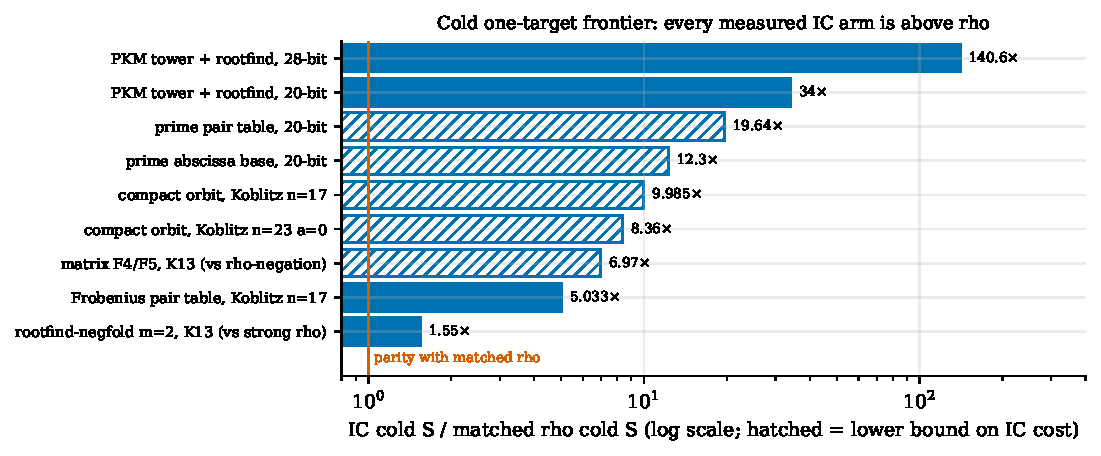
\includegraphics[width=\linewidth]{figures/fig-cold-gap.pdf}
\caption[]{Cold one-target $S$ of index-calculus candidates over their
matched rho arm (each study's own estimator; curves differ, so bars are not
ranked against each other). Hatched: lower bound on IC cost (unpriced
native or solver work). Sources: \art{research/ecbench_frontier_20261013/},
\art{research/ecbench_rootfinding_assessment_20261012/},
\art{research/pkm_tower_ecbench_20261013/},
\art{research/ecbench_rootfind_faster_20261014/}.}
\label{fig:cold}
\end{figure}

\section{What would move the cold frontier}

From the frontier synthesis and the problem records: (i) register the
torsion-symmetrised bases and the $n=83$ dense-root engine in ecbench under
immutable method identities and emit cold and online records; (ii) resolve
the inherited-F4 cross-host counter drift before using that counter in a
bound; (iii) run a four-size native challenge against the standing rho
bound---two sizes cannot establish an exponent; (iv) obtain an isolated
cold session at $n=83$ with every set-up phase and retained byte charged;
(v) price F6-IC's batched geometry with a pinned conversion. Since then
three items have moved to the front: (vi) run $k=4$ over
$\FF_{(2^m)^4}$ at $m=15$--$17$ against a measured negation-map rho, where
the fitted trend predicts parity near $n\approx2^{68}$; (vii) measure the
matched rho on $E_0(\FF_{q^3})$ in the genus-3 rounds' unit (done on 23
October: below rho at $2^{16}$ under the registered pricing, unresolved
elsewhere, \S\ref{sec:transfer}); (viii) obtain a
large-memory host for the $(4,6)$ Weil-descent cell and the PKM tower.
The 21--24 October work adds two more and re-weights one: (ix) measure rho
on the Joux--Vitse cover family at $p\ge503$ (or a size where it can be run)
and emit the cover arm's unpriced counters, so that the $p^{-2}$ trend can be
ranked under the band and tested past $p\approx1330$; (x) define and run a
published-index-calculus reference arm (open problem~10); and (viii) is worth
less than it looked for the binary question, since the $m=4$ row at $w=2$ is
about $+46$ bits over rho even if degree 5 holds (\S\ref{sec:ladder3}).
A result in the cold domain that beats rho at four sizes would be the first
\cls{advance} of the programme.

\chapter{The distance to rho, family by family}\label{ch:distance}

This chapter gives, for each curve family, the current distance between
index calculus and a matched rho. Each figure carries its reference, its
boundary and its validation status. Here a ratio is IC over rho, so
greater than 1 means rho is cheaper. Chapter~\ref{sec:frontier} gives the
frontier campaign, the improvement ladders of 14--24 October, and the
three frontiers (cold, online, stage). This chapter adds the work of
25--29 October and states the position as it stands at the end of the
programme.

\begin{figure}[t]
\centering
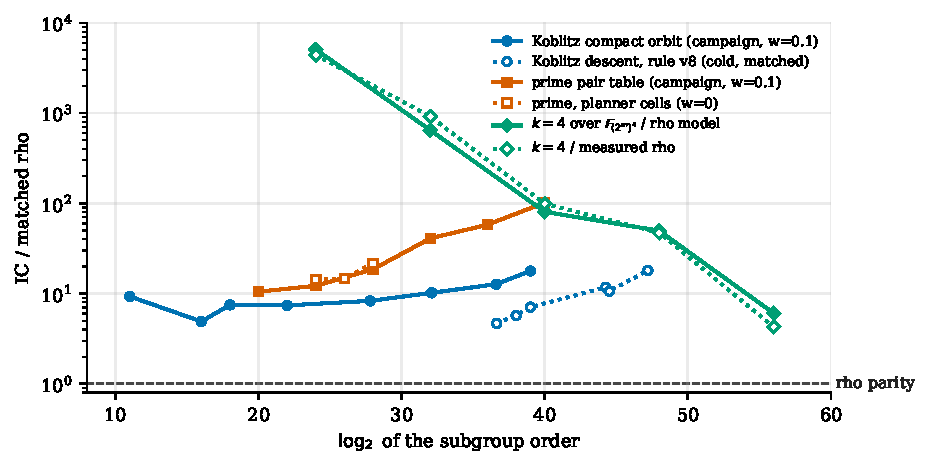
\includegraphics[width=\linewidth]{figures/fig-families.pdf}
\caption[]{Distance to matched rho by family and size. Koblitz and prime
curves: the frontier campaign's priced arms ($w=0.1$, 16 targets $\times$ 2
rounds); open markers are the Koblitz rule at v8 (cold, 64 targets) and the
prime planner cells ($w=0$). $k=4$ over $\FF_{(2^m)^4}$: the characteristic-two
ladder against the negation-map rho model (filled) and a measured rho
(open); the $n\approx2^{56}$ point is one target. Curves and units differ
between families, so the lines are not ranked against each other. Sources:
\art{figures/data-ledger.json}.}
\label{fig:families}
\end{figure}

\section{Koblitz curves}

The leaderboard's Table~A measures a Koblitz descent: aimed $m=3$
collection, then an $m=2$ or $m=3$ descent. It is measured cold on one
unseen public point per process, with 64 points per size, at six sizes
from $2^{36.6}$ to $2^{47.2}$. Figure~\ref{fig:koblitz} shows the rule at
three baselines.
\begin{itemize}
\item \emph{v3 to v7 (same rho).} Index calculus became $1.52$--$1.89\times$
  faster, and the cold ratio fell from $5.23$--$20.97$ to
  $3.43$--$11.5$. The board carries the v7 figures, validated
  (\S\ref{sec:gate}).
\item \emph{v8 (matched rho).} In the same binary, rho's signed-Frobenius
  canonicalisation batched 16 lanes at a time raised the gap by
  $1.30$--$1.58\times$ at every size, to
  \[
    4.67\,[4.34,5.07],\ 5.70,\ 7.07,\ 11.75,\ 10.65,\ 18.07\,[15.98,20.58].
  \]
  All six values lie inside ranges declared before the rows were taken.
  The 408 rows of each run all pass the \texttt{vs\_rho} check
  (\art{research/ic_tool_program/rule/v8/README.md}).
\item \emph{Canonical-step rho (a model).} Pricing rho at the canonical
  batched step gives $6.45$--$23.32\times$ in v8's unit, and
  $9.9$--$43\times$ at rule v4~(\S\ref{sec:ladder3}).
\end{itemize}
The slope of the gap in $\ln r$ is $0.168$ $[0.128,0.208]$ at v8 against
$0.176$ at v3. The v3$\to$v7 improvement lowered the constant, not the
growth.

\begin{figure}[t]
\centering
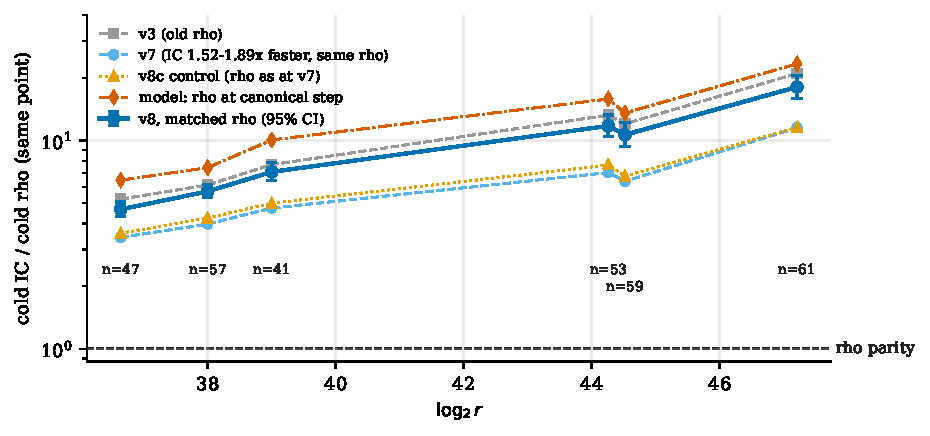
\includegraphics[width=\linewidth]{figures/fig-koblitz-rule.pdf}
\caption[]{The Koblitz rule at three baselines: cold IC over cold rho on the
same public point, 64 targets per size. From v3 to v7 the IC improved
against the same rho. v8 runs the same IC against a matched, faster rho;
its same-binary control, v8c, reproduces v7. The dash-dot line prices rho
at the canonical step. Source:
\art{research/ic_tool_program/rule/v8/README.md}.}
\label{fig:koblitz}
\end{figure}

\paragraph{The priced campaign.} The closest Koblitz arm, compact
Frobenius orbits, is $3.8$--$15\times$ signed-Frobenius rho at $w=0$. Fully
priced against fully priced rho, its best cell is $1.566$ $[0.992,2.347]$;
the ratio is never below 1 and grows as $r^{0.165\,[0.117,0.213]}$.

\paragraph{$n=83$.} The cold pipeline uses the base K1107/root11, which
confirmed a saving of $1.195$\,s $[0.957,1.433]$ on a $115$\,s process (16
public points, GitHub Tier~1 host). The last cold IC/rho ratio is the
K1120 holdout's $55.4$, from five points. A matched precomputed-rho
reproduction on 28 October gave median online IC over rho as follows
(\art{research/n83_k1107_bl_reproduction_20261028/RESULT.md}):
\begin{itemize}
\item $40.9$ $[7.58,141.9]$ against 650\,s table walks;
\item $4.10$ $[1.58,24.8]$ with walks matched to IC set-up;
\item $33.1$ $[6.60,74.4]$ with a table matched to IC memory.
\end{itemize}
Cold, IC took $155.5$\,s against $36.96$\,s for plain rho over all 16
targets. In operation counts the order flips across the pricing band, so
no ranking is made.

\section{Prime curves}

\paragraph{Generic track.} The prime-field programme's owner decisions of
29 October split prime-field index calculus into two counted tracks
(\art{research/prime_ic_program_20261029/DECISIONS.md}):
\begin{itemize}
\item a \emph{generic} track, with table, pair-table and root-finding
  oracles, labelled ``bounded by $\sqrt r$; cannot beat rho'';
\item an \emph{algebraic} track, whose prime baseline is empty.
\end{itemize}
On the generic track:
\begin{itemize}
\item \emph{Table~B} (validated). The prime rows are $5.47$--$13.5\times$
  matched negation rho at 10--24 bits.
\item \emph{Campaign.} The two-summand pair table runs from $10.5\times$
  rho at 20 bits to $101.8\times$ at 40 bits ($w=0.1$). Its fitted
  exponent is $0.620$ $[0.557,0.663]$ against rho's $0.435$, which is the
  $r^{2/3}$ against $r^{1/2}$ of Chapter~\ref{ch:model}.
\item \emph{A $k$-sum table oracle} (28 October,
  \art{research/prime_ksum_table_20261028/}). A negation-folded table of
  every signed 4-sum of a smaller base lowers mean $S$ at $w=0$ by
  $1.9\times$ at 20 bits, rising to $7.2\times$ at 40 bits ($83.7\to11.6$).
  The fitted exponent falls from $0.620$ $[0.586,0.650]$ to $0.521$
  $[0.506,0.538]$, against the theory value $k/(2k-1)=4/7$. That leaves
  $5.3\times$ rho at 20 bits and $13.1\times$ at 40 bits. 2{,}016 runs were
  verified and replayed; the host was L0, and there is no validation.
  The source notes that the method is generic, so its limit is baby-step
  giant-step.
\item \emph{A new 20-bit baseline} (validated,
  \art{research/prime_base_oracle_tuning_20261029/}). Raising the factor
  base from 32 to 45 gives $0.818$ $[0.773,0.866]$ of the incumbent at
  $w=0$. A second host (L2) replayed all 1{,}008 records identically and
  gave $0.836$ $[0.806,0.866]$. The distance to negation rho falls from
  $9.47$ to $7.75$ $[6.92,8.70]$. The same rule at 24 and 28 bits was a
  relabelling, and at 32 bits null.
\item \emph{Planner cells.} These are $12.6$--$25.8\times$ rho.
\end{itemize}

\paragraph{Algebraic track.} The Kummer tower is $28$--$159\times$ rho
(158.9 $[121.6,221.4]$ at 30 bits). No algebraic prime baseline exists.
Its solving degree is the subject of \S\ref{sec:fd-pkm}.

\section{Binary curves of prime degree}

Table~B's random-binary rows are $10.6$--$38.2\times$ matched rho at
$\FF_{2^{15}}$--$\FF_{2^{27}}$, and they are validated. A cofactor-projected
base cuts three of them by $1.29$--$3.36\times$, leaving $6.1$--$14.4\times$.
That base is not yet a board row. For Certicom ECC2-131, the $m=3$ floor
with a free oracle is already above rho~(Chapter~\ref{sec:binary}).

\section{Weak extension-field families}

\begin{figure}[t]
\centering
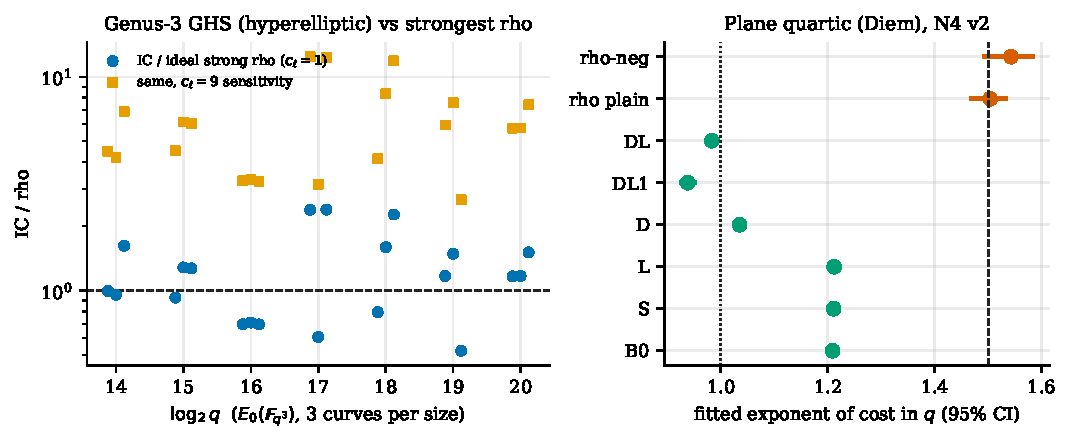
\includegraphics[width=\linewidth]{figures/fig-weak.pdf}
\caption[]{Weak families.
\emph{Left:} genus-3 GHS index calculus (hyperelliptic, double large primes,
round 4) over the ideal strong rho on 21 instances of $E_0(\FF_{q^3})$,
in round 4's unit. Blue: one subgroup multiplication priced at one
$\FF_q$ multiplication, the registered unit. Orange: priced at nine, the
protocol's sensitivity. Below the dashed line IC is cheaper. Source:
\art{research/ghs3_vs_rho_20261023/TABLES.md}.
\emph{Right:} plane-quartic (Diem) index calculus, N4~v2. Fitted exponents
of cold cost in $q$ over $k=8$--$22$ against plain and negation rho, at
$w=0$. Dotted line: $\tilde O(q)$. Dashed line: rho's $q^{3/2}$. Source:
\art{research/quartic_n4v2_20261020/README.md}. Data:
\art{figures/data-new.json}.}
\label{fig:weak}
\end{figure}

Only in these families (Figure~\ref{fig:weak}) does index calculus approach rho or go below it.
\begin{itemize}
\item \emph{Genus 3 via cubic GHS, hyperelliptic route.} This is the
  programme's only preregistered decision of IC below the strongest rho:
  at $q=2^{16}$, IC over the ideal rho reference is $0.70$, $0.71$ and
  $0.70$. At six other sizes the decision is unresolved, and the pooled
  slope is flat ($0.034$ $[-0.047,0.105]$ per bit). Pricing one subgroup
  multiplication at nine $\FF_q$ multiplications puts every instance at
  $2.7$--$12.4\times$ rho (Chapter~\ref{sec:transfer}).
\item \emph{Genus 3 via cubic GHS, plane-quartic route (Diem).} Double
  large primes, structured elimination and Lanczos give a fitted exponent
  of $0.983$ $[0.975,0.993]$ against negation rho's $1.543$. The ratio is
  $0.005$ $[0.004,0.008]$ of negation rho at $q=2{,}097{,}091$, and the
  interpolated crossover is $q^*=555$ $[389,752]$
  (\art{research/quartic_n4v2_20261020/}). The 501 IC units and 2{,}442 rho
  runs are all verified. Three caveats: the host was L0 under heavy load,
  there is no validation file, and the frozen baseline's records do not
  replay. This is a measurement of a known result (Diem, Diem--Thomé).
\item \emph{Joux--Vitse cover of $E(\FF_{p^6})$.} IC is $1.59$--$1.98\times$
  a pooled rho constant at $p=1009$, closing as about $p^{-2}$. This is a
  lower-bound comparison.
\item \emph{$k=4$ over $\FF_{(2^m)^4}$.} IC is $5.2\times$ rho at $m=15$
  after corrections; the crossover is unsupported
  (Chapter~\ref{ch:extension}).
\item \emph{GHS covers over $\FF_{4096}$.} Exact genus-3 covers found by
  search are $549$--$2{,}039\times$ rho in full transfer cost
  (\art{research/ghs_q16_genus3_subcovers_20261028/REPORT.md}).
\end{itemize}

\section{Summary}

\begin{table}[h]
\centering\small
\caption[]{Smallest measured distances to rho, by family.}
\label{tab:nearest}
\begin{tabularx}{\linewidth}{@{}>{\raggedright}p{3.9cm}l>{\raggedright\arraybackslash}X@{}}
\toprule
Family & IC/rho & Qualifier \\
\midrule
Plane quartic via cubic GHS, $q\approx2^{21}$ & $0.005$ & negation rho; weak family; L0; no validation file \\
Genus-3 hyperelliptic via GHS, $q=2^{16}$ & $0.70$ & ideal strong rho; one size of seven; pricing-sensitive \\
Joux--Vitse cover, $p=1009$ & $1.59$--$1.98$ & pooled rho constant; lower bound \\
$k=4$, $\FF_{(2^m)^4}$, $m=15$ & $5.2$ & two targets; crossover unsupported \\
Koblitz, fully priced orbit (best cell) & $1.566$ & never below 1; grows as $r^{0.165}$ \\
Koblitz rule v8, $2^{36.6}$ & $4.67$ & cold, matched, 64 targets \\
Prime, $k$-sum table, 20 bits & $5.3$ & generic track; not validated \\
Prime, Table~B, 12 bits & $5.47$ & validated \\
Random binary, Table~B & $10.6$ & validated \\
Koblitz $n=83$ & $55.4$ & cold, five points \\
\bottomrule
\end{tabularx}
\end{table}

On every prime-order curve of cryptographic shape that the programme
measured, rho is cheaper. Index calculus goes below rho only in weak
extension-field families, which is where theory said it would. There the
programme's contribution is matched, priced, verified measurement of
known algorithms.

\chapter{Corrections and validation}\label{ch:audit}

A ratchet is worth only as much as its pawl. Several recorded results were
corrected once the reference was matched, native work was priced, or the
evidence was replayed. Each correction is recorded in the source with a
dated note; frozen evidence is never rewritten. Figure~\ref{fig:audit}
shows the before and after values. Every correction moved IC's position
against rho \emph{down}, and several moved it from apparently ahead of rho
to behind it.

\begin{figure}[t]
\centering
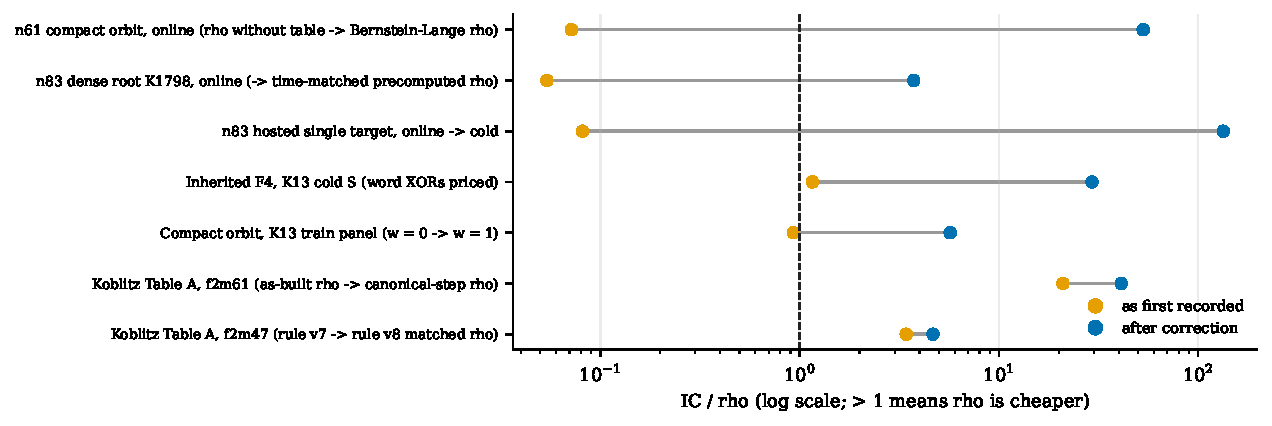
\includegraphics[width=\linewidth]{figures/fig-audit.pdf}
\caption[]{IC/rho as first recorded (orange) and after correction (blue), on
the boundary the correction used. Values left of the dashed line had
claimed IC ahead of rho. Sources: \art{figures/data-ledger.json}.}
\label{fig:audit}
\end{figure}

\section{Claims that did not survive}

\paragraph{1. Every online win is retired.} The one-target online ladder
compared IC \emph{with} a retained table against rho \emph{without} one:
\begin{itemize}
\item $13.94\times$ $[9.81,19.13]$ over strong rho at $n=61$, on 64 targets;
\item $18.53\times$ at $n=83$ with a dense root index;
\item $7.29\times$ and $12.29\times$ on hosted single targets at $n=71$
  and $n=83$.
\end{itemize}
Given a distinguished-point table no larger than IC's pair table,
Bernstein--Lange preprocessing rho~\cite{bl2012} is $53$--$317\times$ faster
online at $n=41,53,61$ on the same 64 targets (benchmarks row
\texttt{20261014-ic-next10-09-equal-advice}). At $n=83$, rho with a table
matched to IC's set-up time or memory wins every pair: $3.74\times$
time-matched and $40.61\times$ memory-matched against K3300, and
$81.5$--$395.5\times$ against K600 (benchmarks row
\texttt{20261016-n83-precomputed-rho-control}). Cold, the hosted $n=83$
point is $133.7\times$ rho. Those online rows measured what a table buys,
and generic rho buys more per byte. The within-IC result survives: K1798's
probe reduction over K1500 at $n=83$ (from $300{,}021.9$ to $169{,}069.8$
probes per relation).

\paragraph{2. Pricing native work moved two arms.}
\begin{itemize}
\item \emph{Inherited F4 at $n=13$.} Its $S=16.7$, close to rho's $14.4$,
  left its Boolean word XORs unpriced. Priced, $S=421.4$
  (\art{research/ecbench_rootfind_faster_20261014/}).
\item \emph{F4 pricing change.} The pricing change (\#1774, $0.002304$ GAE
  per word XOR) made every earlier F4 $S$ a lower bound. A separate
  algorithmic change (\#1862) raised counted work
  (\art{research/f4_pricing_jump_20261018/README.md}).
\item \emph{Compact orbit at $n=13$.} Earlier quoted at $1.08\times$ rho as a
  lower bound, it reads $0.93$, $1.53$ and $5.7\times$ the strong rho at
  $w=0,0.1,1$, so the pair is unresolved inside the band
  (\art{research/ic_frontier_campaign_20261015/select/SELECTION.md}).
\end{itemize}

\paragraph{3. Matching the rho reference.}
\begin{itemize}
\item \emph{Rule v8.} Matching the rho reference raised the Koblitz gap by
  $1.30$--$1.58\times$ at every size (Chapter~\ref{ch:distance}).
\item \emph{The standing rho improved.} Ecbench's standing
  \texttt{rho.signed\_frobenius\_strong} now runs at $0.802\times$ its
  former instruction count with identical GAE, and the strong Koblitz rho
  executes 718 instructions per step instead of 1{,}196. Counted-unit
  comparisons are unaffected. Wall-time comparisons against the older rho
  overstate IC by up to that factor.
\item \emph{Two rho studies on the prime side.} Choosing the better of
  $P\pm R$ cuts steps by $1.129\times$. Signed $\sigma$ steps on
  ECC2K-130 cut GPU time to $0.961$--$0.970$. Neither is yet in a campaign
  arm.
\end{itemize}

\paragraph{4. A replay regression, and its root cause.} The root-finder
ecbench session was recorded with a replay certificate of 120 of 168
identical records; the 48 mismatches were all in inherited F4's word-XOR
counts. On \texttt{main} of 19 October it replayed only 72 of 168, with
mismatches in all four index-calculus arms.
\begin{itemize}
\item \emph{First diagnosis} (20 October). A cross-ISA replay found that
  with the x86-only BMI2 branch disabled, x86 reproduces all 168 of 168
  records, and so does an aarch64 build under emulation
  (\art{research/validation_sweep_20261019/D-known-issues/item1_cross_isa_20261020/RESULT.md}).
\item \emph{Cause, stated precisely} (26 October addendum). At the recorded
  commit, BMI2 availability decided whether F4's row specialisation was
  \emph{eager} (every kept row rewritten at once and charged per row) or
  \emph{lazy} (rewritten on first read). The two differ in the quantity
  charged, for example $301{,}961$ against $300{,}531$ word XORs. Since
  \#2043 every host is eager and the two eager paths charge identical
  counts. Sessions now record the version of the F4 accounting they were
  made under
  (\art{research/validation_sweep_20261019/D-known-issues/ADDENDUM-20261026-item1-accounting.md}).
\end{itemize}
Archived sessions recorded with the lazy charge cannot replay on
\texttt{main}. That is a change of definition, not a dependence on the host.
Scalars, trial counts and charged group operations are unaffected.

\paragraph{5. Reported cells that compared unlike statistics.} The
u64-rootbatch rank and per-target cells compared a fastest run with a
median, and were corrected from $2.95\times$ and $6.09\times$ to $2.47\times$
and $5.00\times$ (Chapter~\ref{sec:koblitz}). The $n=83$ stacked producer's
``$360\to94.4$'' cold-gap history mixed a ratio from another run; paired
within the run it is $305.8\to94.4$ (Chapter~\ref{sec:koblitz}).

\paragraph{6. Results resting on faulty code or wrong references.}
\begin{itemize}
\item \emph{Plane-quartic IC.} Its $S$ values of $650{,}896$ to
  $3.79\cdot10^7$ rest on a degree-3 reduction in
  \art{research/ghs_cubic_quartic_ic_20261012/quartic_ic.rs} that merges
  distinct classes (reported in an open pull request). Recoveries are still
  checked against the planted scalar, but relation counts and $S$ are
  unverified.
\item \emph{Volcano census crater.} A claim that IC is 22--25\% cheaper on
  the volcano crater was withdrawn, because the crater's rho reference
  should have been the cubic-automorphism rho. Against it, IC is
  $84.9\times$ rho at $w=0$
  (\art{research/volcano_ecdlp_census_20261017/REPORT.md}, erratum A3).
\end{itemize}

\paragraph{Reading.} None of these corrections removes an IC improvement
against its own incumbent. They correct the \emph{distance to rho}, which
is the quantity most exposed to an unmatched reference or an unpriced
counter. This is why the gate of \S\ref{sec:gate} asks for a matched,
band-priced rho on every row.

\section{Validation status}\label{sec:gate}

Since 19 October no row may enter the index-calculus leaderboard or
\art{benchmarks/README.md} without three pieces of evidence, named by the
evidence directory's \texttt{VALIDATION.json}
(\art{docs/VALIDATION_GATE.md}):
\begin{itemize}
\item an independent replay certificate with verified scalars;
\item an independent validator report that recomputes every headline
  number;
\item a matched rho reference: the strongest available, in the same unit
  and the same binary, priced across the §5a band.
\end{itemize}
On 29 October, \textbf{19 of the 28 leaderboard rows are validated}
(\art{docs/ic/leaderboard.json}, \texttt{validation\_gate.status\_counts}).

\begin{itemize}
\item \emph{Table~B, all 13 rows (prime and random binary, one target).}
  These validated on 24 October
  (\art{research/ic_validation_gate_20261024/}):
  \begin{itemize}
  \item 1{,}257 runs replay identically in a fresh process;
  \item 1{,}578 of 1{,}578 negative controls are rejected by an
    independent verifier;
  \item 52 headline numbers recompute to relative $10^{-9}$;
  \item index calculus stays above rho at every band weight.
  \end{itemize}
  Its distance is $5.47$--$38.21\times$ the matched negation-map rho, or
  $4.05$--$54.76\times$ across the band.
\item \emph{Table~A, all 6 rows (Koblitz descent, one target, 64 targets per
  size).} These validated at baseline v7
  (\art{research/ic_tool_program/rule/v7/}): IC is $3.43$--$11.5\times$ the
  as-built rho in the same process. The sweep flags the reference as only
  partly adequate. Against the matched rho of rule v8, the same rows read
  $4.67$--$18.07\times$ (Chapter~\ref{ch:distance}).
\item \emph{Table~C, all 9 rows (32-target batch).} These stay pre-gate.
  Their replays and recomputations pass, but no matched rho with a band
  exists for them.
\item \emph{Components outside Tables A--C.} Two are validated: the
  prime-field base-size tuning and the post-Gröbner linear stage
  (\art{research/prime_base_oracle_tuning_20261029/VALIDATION.json},
  \art{research/postgb_linear_stage_20261026/validation/VALIDATION.json}).
\end{itemize}
Validation says the numbers are what the archive says, and that the
reference is fair. \textbf{No validated row is below its reference.}

The theory of Part~\ref{part:theory} has a different standard of evidence:
\begin{itemize}
\item written proofs, which still need expert review;
\item independently checked certificates;
\item Lean for the finite and algebraic identities only.
\end{itemize}
Each theorem there names its tier.


\part{Outlook}\label{part:outlook}
\chapter{Open problems and proposed experiments}\label{sec:open}

% Survey section (draft 2026-10-15). Each problem is phrased as the
% measurement or proof that would settle it, per the repository's
% "name the obstruction" rule.

\paragraph{1. The solving degree of Weil-descended summation systems.}
Every subexponential claim for prime-degree binary curves rests on a bound
for this degree (\S\ref{sec:theory}); none is proved and the experimental
evidence is contested. \emph{Experiment:} measure first-fall, last-fall
and solving degree of $\Sem{m+1}$ restricted to $\ell$-dimensional
subspaces over a grid of $(n,\ell,m)$ with $m\ge3$, at least four values
of $n$ per $(\ell,m)$, against the semi-regular prediction, with
multi-graded regularity (one block per summand) as a second model.
\emph{Settles:} whether the degree grows with $n$ at fixed $(\ell,m)$; a
growth consistent with zero would revive the Petit--Quisquater and Semaev
heuristics, a positive slope would close them for this model.

\paragraph{2. Cold index calculus against rho with every operation
priced.} No measured arm beats matched rho on the cold one-target boundary
once native work is priced on both sides (\S\ref{sec:frontier}).
\emph{Experiment:} the frontier campaign of \S\ref{sec:frontier} extended
to the largest sizes each arm can reach, with exponents fitted per arm and
the crossover reported only where the fitted exponents separate across the
whole pricing band. \emph{Settles:} whether any implemented arm has an
exponent below $1/2$ in $r$ on these families.

\paragraph{3. Relation yield is now the dominant stage.} Root finding made
the decomposition oracle cheap; what remains is the number of trials per
relation, governed by the factor-base density. \emph{Experiment:} for each
factor-base family, the measured trials-per-relation law against $r$ and
base size, compared with the counting prediction $m!\,r/N^{m-1}$; the
residual (e.g.\ the unexplained factor 5 in the ECC2K-130 extrapolation,
\S\ref{sec:koblitz}) is the target.

\paragraph{4. Root finding beyond two summands on prime curves.} The
two-summand oracle is prior art in mechanism (McGuire--Mueller) and costs
$\Theta(N)$ per trial; three summands cost a pair table of $N^2$ entries.
\emph{Question:} is there a sub-$N^2$ structure for $\Sem4$ membership
over a prime-field base---for example from the $D_m$-invariant coordinates
of 2-torsion curves---and does it change the $r^{2/3}$ cost of two-summand
prime index calculus? A negative answer with a counting argument would be
as useful as a positive one.

\paragraph{5. The preprocessing regime.} Index calculus with a retained
table beats rho without one, and loses by $53$--$317\times$ to
Bernstein--Lange rho with an equal or smaller table (\S\ref{sec:ladder}).
\emph{Experiment:} measure the advice--time curve $(S,T)$ of the
compact-orbit arm across sizes against preprocessing rho's
$S\,T^2\approx N$; an index-calculus online result counts only if it lies
below that curve at equal $S$.

\paragraph{6. Symmetry at $k=4$, end to end.} The $D_4$ reduction and its
four-unknown weighted form move a \emph{modelled} handover over $\FF_{p^4}$
from about $2^{150}$ to $2^{119}$--$2^{137}$ depending on frame
(\S\ref{sec:ladder}).
Since then the odd-characteristic oracle is $370\times$ cheaper again
(index calculus still $1.39\cdot10^6\times$ rho), and in characteristic two
a Frobenius-reduced form brings the measured gap to $6.1\times$ rho at
$n\approx2^{56}$, closing as $n^{-1/4}$ (\S\ref{sec:ladder2}).
\emph{Experiment:} continue the characteristic-two ladder to $m=15$--$17$
with a measured negation-map rho at every rung, cold and priced across the
band; a measured crossover near $n\approx2^{68}$ would confirm the fit, and
its absence would locate the term the model misses. A red-team review
(Chapter~\ref{ch:extension}) found the only clean point, $m=15$, at
$5.2\times$ rho after corrections and placed the crossover at
$m^*\approx17.6$ ($16.3$--$19.2$); its frozen replication plan (eight targets
per arm, $m=14$--$17$, about 30\,h) is the experiment to run.

\paragraph{7. Pricing and calibration infrastructure.} Rankings now
require every arm's native work to be counted (AGENTS.md \S5a).
\emph{Work:} count the three uncounted categories of the shared-rank arm;
calibrate every ladder size on one fixed host; record the inherited-F4 code
path (BMI2 or portable) in its method identity, now that the cross-host
counter drift is traced to it; register the $n=83$ dense root index in the
harness.

\paragraph{8. Genus three after cubic GHS, to the crossover.} The one
family whose fitted exponent (about $q^{1.4}$) lies below rho's $q^{3/2}$ was
$1.15\times$ a measured negation-map rho at $q=2^{20}$ before rounds three
and four cut a further $0.44\times$ (\S\S\ref{sec:ladder},\ref{sec:ladder2}),
and is now below the strongest rho at $q=2^{16}$ under the registered
pricing, unresolved at the other sizes to $2^{20}$, and above it under a
heavier sensitivity pricing, with no measurable pooled trend
(\S\ref{sec:transfer}). What would settle it is the same comparison at
$q=2^{21}$--$2^{24}$ on instances of one cofactor, with the subgroup
multiplication's price measured rather than chosen;
its local exponent is down to $1.356$, still above $4/3$ because the linear
algebra grows faster than $q^{4/3}$, and $q=2^{23}$ needs more than the
4.5\,GB cap.
\emph{Experiment:} measure negation-map rho on the same instances in the
latest unit (inversions and mod-$\ell$ multiplications priced), and run
both past $q=2^{22}$, in the harness and across the pricing band. A measured
crossover there would be the programme's first \cls{advance} against rho,
on a narrow and undeployed family.

\paragraph{9. Plane quartics: Diem's $\tilde O(q)$.} Genus-3 GHS covers whose
Jacobian is that of a smooth plane quartic admit Diem's index
calculus~\cite{diem2006,dt2008} at $\tilde O(q)$, against $\tilde O(q^{4/3})$ for
the hyperelliptic route and $q^{3/2}$ for rho on $E(\FF_{q^3})$. The
repository builds such quartics directly ($m=2$ GHS, toy index calculus at
$q\le11$) and through Smith's $(2,2,2)$-isogeny from the hyperelliptic case
(18.6\% of random curves); a four-workstream programme was scoped on 18
October (\art{research/plane_quartic_program_20261018/PROGRAM.md}).
\emph{Experiment:} the hyperelliptic ladder's instances, carried to plane
quartics where Smith's conditions pass, with Diem's relation search and the
same linear algebra, against the same matched rho. The 23 October literature
round ranks this branch as its one exponent candidate (LEAD-15,
\art{research/pdp_literature_leads_20261022/}).
\emph{Since then:} the arithmetic has been rebuilt with canonical class keys,
which resolve the degree-3 merges (\S\ref{sec:corrections}). On the direct
quartic route, index calculus is below a matched plain rho from $q=4051$,
with fitted exponent $1.083$ against $1.485$, and N4~v2 extends this
against a negation-map rho to $q\approx2^{22}$, at exponent $0.983$ and
$0.005\times$ rho (\S\ref{sec:transfer}). \emph{Still open:} a validation
of N4~v2 on an isolated host with a replayable baseline; index calculus on
the quartics reached through Smith's isogeny; and a record-scale run (for
example $q\approx2^{40}$, $\ell\approx2^{120}$) where rho is out of reach
and the published Diem--Thomé timings are the comparator.

\paragraph{10. A published index calculus as the reference arm.} Every
ratio in this treatise is against rho or the programme's own previous arm;
none is against the state of the art in index calculus at the same
$(q,n,m)$ (\S\ref{sec:ladder3}). \emph{Work:} fix, per curve and size, the
standard base $\{P:x(P)\in\FF_q\}$, the FGHR-symmetrised summation
polynomial (2-torsion and, on Koblitz curves, Frobenius invariants), msolve
as the solver and WDSat for binary decompositions, and run it in ecbench
on the existing ladders (binary $n=13$--$37$, Koblitz $n=41$--$61$, $k=4$
extension fields). \emph{Settles:} whether any engineering result of
\S\S\ref{sec:rootfinding}--\ref{sec:transfer} improves on published index
calculus, as opposed to on this programme's own baseline. Stage ratios
quoted against the in-house F4 say nothing about published Gr\"obner
engines until this is done.

\paragraph{11. The Joux--Vitse cover, to the crossover.} The cover of
$E(\FF_{p^6})$ closes on rho as about $p^{-2}$ and is $1.6$--$2.0\times$ a
pooled rho constant at $p=1009$, with the line meeting rho near
$p\approx1330$ by extrapolation (\S\ref{sec:ladder3}). \emph{Experiment:}
emit the cover arm's unpriced F4 and Wiedemann counters, measure rho at the
largest $p$ it can run (or with a memory-light rho at $p\ge503$), and run
both at $p\approx1300$--$2000$, across the band. A measured crossover would
be the programme's first \cls{advance} against rho, on a weak and undeployed
class; its absence at the predicted $p$ would locate the term the cost
model misses.

\paragraph{12. A growing lower bound on the last fall degree.} Chapter~\ref{ch:falldegree}
proves the first fall degree constant and certifies $d_F\ge5$ on named
binary instances, but no presentation has a proved lower bound that grows
with $n$ or $k$. \emph{Proof route:} construct degree-$c$ pseudo-solutions,
i.e.\ linear functionals on $B_{\le c}$ that kill $W_c(F)$ and not 1, for a
family of instances, generalising the closure certificates of
Proposition~\ref{prop:cert}. The regular closure pattern observed (exactly
$4n$ new cubic dimensions per round, then a stall) and the
iterated-system lower-bound technique of~\cite{iterated2023} are the
starting points. \emph{Settles:} the open problem of
HKY~\cite{hky2015} and Kousidis--Wiemers~\cite{kousidis2019}; a bound
$\omega(\sqrt{n\ln n})$ would invalidate the subexponential conclusion of
Semaev's analysis for these systems.

\paragraph{13. Certificates at scale.} \emph{Experiment:} certify
$1\notin W_4$ (and, where it holds, $1\notin W_5$) on about ten random and
ten polynomial subspaces per $n$ for $n=33$--$51$, publish the
certificates, and extend the guarded chain to $B=4$--$8$ by computation.
\emph{Settles:} whether the step $4\to5$ is a population property, and
where $5\to6$ occurs; the exact $d_F$ of the guarded chain beyond $B=3$.

\paragraph{14. The prime-field Kummer tower, re-measured.} The session
values $d_F=3,4,4,4,4,5,5,5,5,6$ at $t=1..10$ were never committed.
\emph{Experiment:} regenerate stage A at $t=1..14$ with closure
certificates and score the registered prediction
$d_F=4+\lfloor(t-2)/4\rfloor$; extrapolated F4 times are about 1.7\,h, 17\,h
and 7 days at $t=12$--$14$ (\art{research/prime_ic_program_20261029/}).
\emph{Settles:} whether the proved constant first fall degree 4 sits beside
a last fall degree that keeps growing in the setting PKM introduced.

\chapter{Conclusion}\label{ch:conclusion}

Four months of work on elliptic-curve index calculus produced four kinds of
result.

\paragraph{Theory.}
\begin{itemize}
\item \emph{What is fixed for every curve.} The summation cover's monodromy
  is $(\ZZ/2)^{m-2}$ everywhere. Its fibres split completely where relation
  search operates. The mean yield at a given base size is a double count.
  So no choice of curve or base geometry can raise the \emph{mean}
  decomposition yield at matched base size. Coverage, the cost of the
  membership oracle and the difficulty of the solve remain free, and the
  engineering of Part~\ref{part:algorithms} works on those.
\item \emph{What is open.} For three presentations of the decomposition
  system the first fall degree is a constant of the presentation, and the
  last fall degree is not bounded by it:
  \begin{itemize}
  \item proved for the guarded chain;
  \item certified on named instances of binary Weil descent;
  \item measured for prime-field Kummer towers.
  \end{itemize}
  The subexponential claims for binary curves assume exactly the step
  these results show is not automatic. Whether the last fall degree grows
  without bound is unproved.
\end{itemize}

\paragraph{Engineering.} The decomposition oracle became two to five
orders of magnitude cheaper where root finding applies. The Gröbner
engines improved by one to two orders in counted work. Factor bases
closed under known-logarithm maps, a $k$-sum table, and set-up and linear
algebra engineering each cut a constant. None of this changed an exponent
on a prime field or a prime-degree binary field. The prime-field $k$-sum
oracle moved its exponent from $0.62$ to $0.52$, but it is generic, and
its limit is baby-step giant-step.

\paragraph{Measurement.} At a matched reference, priced across a band and
replayed, rho is cheaper on every prime-order curve the programme measured:
\begin{itemize}
\item $4.7$--$18\times$ on Koblitz curves of 37--47 bits;
\item $5.3$--$102\times$ on prime curves of 20--40 bits;
\item $10.6$--$38\times$ on random binary curves.
\end{itemize}
Nineteen leaderboard rows passed a validation gate that demands independent
replay, recomputation and a matched rho. None of them is below its
reference. Every online win disappeared under an equal-advice audit, and
the corrections forced by matching, pricing and replaying lengthened the
measured distance more often than any single improvement shortened it.

\paragraph{Where index calculus wins.} In weak extension-field families
($E_0/\FF_{q^3}$ through genus-3 covers, Joux--Vitse covers of
$E(\FF_{p^6})$, and perhaps $k=4$ in characteristic two) the measured cost
crosses or approaches rho, as theory predicts. The plane-quartic route
measured exponent $\approx1$ against rho's $1.5$, at $0.005\times$ negation
rho near $q=2^{21}$. These are known algorithms; the programme's
contribution there is fair measurement.

\paragraph{What would change the picture.} Three items, in order of what
they would settle:
\begin{enumerate}
\item \emph{A proved lower bound on the last fall degree that grows with
  $n$}, for any presentation of the binary decomposition system. It would
  answer the question left open by Huang, Kosters and Yeo and by
  Kousidis and Wiemers, and it is the only result that bears on the
  subexponential claims.
\item \emph{More certified instances} at $n=33$--$51$, with public
  certificates, to show whether the last fall degree reaches 6.
\item \emph{The frozen $k=4$ replication} at $m=14$--$17$, the cheapest
  experiment that could put a measured crossover on record. It would be
  in a weak family.
\end{enumerate}
Nothing here concerns a deployed curve. The open problems of
Chapter~\ref{sec:open} state each remaining question as the experiment or
proof that would settle it.


\appendix
\chapter{Artefacts}\label{app:artefacts}

Every number in this treatise is copied from a committed artefact. The
treatise ran one re-verification (\S\ref{sec:fd-binary}) and no new
measurement. Artefact paths are relative to the \texttt{crypto} repository
unless prefixed \texttt{crypto-autoresearcher:}.

\paragraph{Companion documents.}
\begin{itemize}
\item \art{papers/ecdlp-index-calculus-program/}~\cite{icprogram2026} is
  the chronological record, with study catalogues for both repositories
  (about 1{,}400 directories) and the list of open pull requests. Where this
  treatise reuses its chapters (background, literature, measurement, root
  finding, Gröbner engines, Koblitz, binary and prime curves, transfers,
  frontier, open problems), the text is that record's as of 26 October,
  updated where later evidence changed a number.
\item \art{papers/ecdlp-ic-improvement-ledger/}~\cite{icledger2026} is the
  ratchet of incumbents to 23 October.
\item \art{research/paper_opportunities_20261029/} is the assessment that
  identified the fall-degree results of Chapter~\ref{ch:falldegree} as the
  programme's strongest theory, and that holds the certificate
  re-verification.
\end{itemize}

\paragraph{Theory (Part~\ref{part:theory}).}
\begin{itemize}
\item \art{crypto-autoresearcher:papers/semaev-conservation-specialization/}
  (Chapter~\ref{ch:cover}).
\item \art{crypto-autoresearcher:analysis/semaev-m2-last-fall-degree/}:
  \texttt{theorem-dossier.md}, \texttt{results/}, and \texttt{verify/}
  (\texttt{cert\_check.py}, \texttt{b\_sweep.py}).
\item \art{research/guarded_fall_degree_20261028/}: \texttt{proofs/},
  \texttt{extensions/}, \texttt{native/}, \texttt{formal/}.
\item \art{research/prime_fall_degree_20261027/DERIVED.md}.
\item \art{crypto-autoresearcher:papers/nagao-lemma4-note/} and
  \art{crypto-autoresearcher:docs/reports/2026-10-22-semaev-first-fall-replay/}.
\item \art{crypto-autoresearcher:knowledge/leads/ecdlp/} (Chapter~\ref{ch:obstructions}),
  \art{research/twist_obstruction_20261026/} and
  \art{research/lift_dense_factor_base_20261027/}.
\end{itemize}

\paragraph{The summer record (Chapter~\ref{ch:summer}).}
\begin{itemize}
\item \art{research/ecdlp_jul_sep_index_20261029/}: \texttt{INDEX.json},
  \texttt{INDEX.tsv}, \texttt{SUMMARY.json}, \texttt{build\_index.py}.
  Each row cites its \art{crypto-autoresearcher:ledger/decisions/} file
  and the \texttt{experiments/EXP-*/runs/} directories of its targets.
\end{itemize}

\paragraph{Late measurements (Chapters~\ref{ch:extension}--\ref{ch:audit}).}
\begin{itemize}
\item \art{research/gaudry_k4_char2_redteam_20261026/REPORT.md}.
\item \art{research/quartic_n4v2_20261020/} and \art{research/ghs3_vs_rho_20261023/}.
\item \art{research/prime_ksum_table_20261028/} and
  \art{research/prime_base_oracle_tuning_20261029/}.
\item \art{research/prime_ic_program_20261029/}.
\item \art{research/n83_k1107_bl_reproduction_20261028/}.
\item \art{research/ghs_q16_genus3_subcovers_20261028/}.
\item \art{research/postgb_linear_stage_20261026/}.
\item \art{research/ic_validation_gate_20261024/}, \art{docs/ic/LEADERBOARD.md}
  and \art{docs/ic/leaderboard.json}.
\end{itemize}

\paragraph{Figures.} The figures of the programme record and the ledger are
copied with their data (\art{figures/data-program.json},
\art{figures/data-ledger.json}); their plotting scripts live in those
papers' directories. The new figures (fall degrees, weak families) are
rendered by \art{figures/make_fig_fall_degrees.py} and
\art{figures/make_fig_weak.py} from \art{figures/data-new.json}. That file
holds recorded values only, each with its source.


\bibliographystyle{plainnat}
\bibliography{refs}

\end{document}
